% Options for packages loaded elsewhere
\PassOptionsToPackage{unicode}{hyperref}
\PassOptionsToPackage{hyphens}{url}
%
\documentclass[
  12pt,
]{article}
\usepackage{amsmath,amssymb}
\usepackage{iftex}
\ifPDFTeX
  \usepackage[T1]{fontenc}
  \usepackage[utf8]{inputenc}
  \usepackage{textcomp} % provide euro and other symbols
\else % if luatex or xetex
  \usepackage{unicode-math} % this also loads fontspec
  \defaultfontfeatures{Scale=MatchLowercase}
  \defaultfontfeatures[\rmfamily]{Ligatures=TeX,Scale=1}
\fi
\usepackage{lmodern}
\ifPDFTeX\else
  % xetex/luatex font selection
\fi
% Use upquote if available, for straight quotes in verbatim environments
\IfFileExists{upquote.sty}{\usepackage{upquote}}{}
\IfFileExists{microtype.sty}{% use microtype if available
  \usepackage[]{microtype}
  \UseMicrotypeSet[protrusion]{basicmath} % disable protrusion for tt fonts
}{}
\makeatletter
\@ifundefined{KOMAClassName}{% if non-KOMA class
  \IfFileExists{parskip.sty}{%
    \usepackage{parskip}
  }{% else
    \setlength{\parindent}{0pt}
    \setlength{\parskip}{6pt plus 2pt minus 1pt}}
}{% if KOMA class
  \KOMAoptions{parskip=half}}
\makeatother
\usepackage{xcolor}
\usepackage[a4paper, margin=1in]{geometry}
\usepackage{graphicx}
\makeatletter
\newsavebox\pandoc@box
\newcommand*\pandocbounded[1]{% scales image to fit in text height/width
  \sbox\pandoc@box{#1}%
  \Gscale@div\@tempa{\textheight}{\dimexpr\ht\pandoc@box+\dp\pandoc@box\relax}%
  \Gscale@div\@tempb{\linewidth}{\wd\pandoc@box}%
  \ifdim\@tempb\p@<\@tempa\p@\let\@tempa\@tempb\fi% select the smaller of both
  \ifdim\@tempa\p@<\p@\scalebox{\@tempa}{\usebox\pandoc@box}%
  \else\usebox{\pandoc@box}%
  \fi%
}
% Set default figure placement to htbp
\def\fps@figure{htbp}
\makeatother
\setlength{\emergencystretch}{3em} % prevent overfull lines
\providecommand{\tightlist}{%
  \setlength{\itemsep}{0pt}\setlength{\parskip}{0pt}}
\setcounter{secnumdepth}{-\maxdimen} % remove section numbering
\usepackage{setspace}
\usepackage{newtxtext}
\doublespacing
\usepackage{booktabs}
\usepackage{longtable}
\usepackage{array}
\usepackage{xcolor}
\usepackage{pdflscape}
\newcommand{\blandscape}{\begin{landscape}}
\newcommand{\elandscape}{\end{landscape}}
\usepackage{afterpage}
\usepackage{chngcntr}
\counterwithout{figure}{section}
\counterwithout{table}{section}
\renewcommand{\contentsname}{}
\renewcommand{\listtablename}{}
\renewcommand{\listfigurename}{}
\usepackage{etoolbox}
\usepackage{tocloft}
\usepackage{titlesec}
\titleformat{\section}{\normalfont\large\bfseries\filcenter}{\thesection}{1em}{\MakeUppercase}
\titleformat*{\section}{\normalfont\large\bfseries\filcenter\MakeUppercase}
\titlespacing*{\section}{0pt}{*3}{*2}
\renewcommand{\cftsecnumwidth}{2em}
\renewcommand{\cftsubsecnumwidth}{2em}
\setlength{\skip\footins}{20pt}
\usepackage[style=apa, backend=biber]{biblatex}
\usepackage{url}
\usepackage{parskip}
\setlength{\parskip}{0pt}
\setlength{\parindent}{2em}
\usepackage{indentfirst}
\usepackage{fancyhdr}
\pagestyle{fancy}
\fancyhf{}
\fancyhead[L]{Joonghoe KIM}
\fancyhead[C]{KDI School of Public Policy and Management}
\fancyhead[R]{Thesis}
\fancyfoot[C]{\thepage}
\renewcommand{\headrulewidth}{0pt}
\usepackage{float}
\usepackage{placeins}
\usepackage[justification=centering]{caption}
\usepackage{booktabs}
\usepackage{longtable}
\usepackage{array}
\usepackage{multirow}
\usepackage{wrapfig}
\usepackage{float}
\usepackage{colortbl}
\usepackage{pdflscape}
\usepackage{tabu}
\usepackage{threeparttable}
\usepackage{threeparttablex}
\usepackage[normalem]{ulem}
\usepackage{makecell}
\usepackage{xcolor}
\usepackage[]{biblatex}
\addbibresource{reference.bib}
\nocite{*}
\usepackage{bookmark}
\IfFileExists{xurl.sty}{\usepackage{xurl}}{} % add URL line breaks if available
\urlstyle{same}
\hypersetup{
  hidelinks,
  pdfcreator={LaTeX via pandoc}}

\author{}
\date{\vspace{-2.5em}}

\begin{document}

\newpage
\thispagestyle{empty}
\null
\newpage
\begin{titlepage}
\thispagestyle{empty}
    \centering
    {\large \textbf{\parbox{\textwidth}{\centering Burnout from Overwork: Job Disutility under Industrial Labor Shortage}}} \\[2.5cm]

    {By} \\[0.5cm]
    \textbf{KIM, Joonghoe} \\[3cm]

    \textbf{A THESIS} \\[2.5cm]

    Submitted to \\[0.5cm]
    \textbf{KDI SCHOOL OF PUBLIC POLICY AND MANAGEMENT} \\[0.5cm]
    
    In Partial Fulfillment of the Requirements \\[0.5cm]
    For the Degree of \\[0.5cm]
    \textbf{MASTER OF PUBLIC POLICY} \\[3cm]

    \textbf{2025}
\end{titlepage}
\newpage
\begin{titlepage}
\thispagestyle{empty}
    \centering
    {\large \textbf{\parbox{\textwidth}{\centering Burnout from Overwork: Job Disutility under Industrial Labor Shortage}}} \\[2.5cm]

    {By} \\[0.5cm]
    \textbf{KIM, Joonghoe} \\[2.5cm]

    \textbf{A THESIS} \\[1cm]

    Submitted to \\[0.5cm]
    \textbf{KDI SCHOOL OF PUBLIC POLICY AND MANAGEMENT} \\[0.5cm]
    
    In Partial Fulfillment of the Requirements \\[0.5cm]
    For the Degree of \\[0.5cm]
    \textbf{MASTER OF PUBLIC POLICY} \\[2cm]

    \textbf{2025}

    Professor SHIN, Jaeun (Supervisor) \\[0.5cm]

\end{titlepage}
\newpage
\cleardoublepage
\pagenumbering{roman}
\setcounter{page}{1}

\section*{ABSTRACT}\label{abstract}
\addcontentsline{toc}{section}{ABSTRACT}

\thispagestyle{empty}

\begin{center}

\vspace{1em}

\textbf{BURNOUT FROM OVERWORK:} \\
\textbf{JOB DISUTILITY UNDER INDUSTRIAL LABOR SHORTAGE}

\vspace{1em}

By Joonghoe KIM
\end{center}

\vspace{2em}

\setlength{\parindent}{0pt}

Long working practices in Korea are often regarded as a reflection of
less productive and hazardous work environments compared to other OECD
countries. Meanwhile, occupational fatigue has conventionally been
attributed to personal choices such as poor self-management or overly
ambitious intentions. This paper aims to clarify that individual
negative perception of excessive working experiences is not limited to
personal differences or irrational responses. Predominant market
constraints lead to selection distortion, and its impact is related to
the misallocation of labor. Thus, the presenting analysis argues that
the skewed allocation of labor reflects individual Burn-out syndrome,
induced by pressured overwork. Foundational to the given conceptual
framework, the Two-Staged Predictor-Substitution (2SPS) estimation was
structured. First, labor shortage rates reported at each of 16
industrial categories, 5 categories of firm size, and 17 regions
externally impact individual working hours. Subsequently, excessive
working hours interrupt individual utility maximization, contrasted to
the generally accepted view that the observed working hours represent an
optimized laborer decision. Previous literature mainly focused on the
internal variation of determinants in the short term, however, this
study incorporates structural constraints to correct endogenous working
hour decisions with mid-to-long-term labor market data. Using 15 years
of data aggregated from both the Korean Labor and Income Panel Study
(KLIPS) and the Occupational Labor Force Survey at Establishments
(OLFSE), empirical estimation was held on 52,418 observations of 12,141
individuals aged 18-65. Concerning the Average Causal Response (ACR)
theorem in non-linear model applications based on Conditional Maximum
Likelihood (CML), the causal estimates reveal constrained overtime
decisions under labor shortage circumstances and their causal effects.
First, a 1\%p increase in labor shortage rates imposes 0.1573 working
hours on average, except for less labor-intensive industries. As
responses to the first stage estimates, a 0.5\%p decrease in odds of
maximizing their utility per hour for affected overtime workers.
Therefore, this paper calls for the need to address persistent labor
market rigidity rather than simply imposing further regulatory measures.

\setlength{\parindent}{2em}

\thispagestyle{empty}

\newpage

\thispagestyle{empty}

\begin{center}
\vspace*{\fill}

\large \textit{To Jesus Christ, who promised us, “Peace be with you.”}

\vspace{1em}

\rule{0.6\linewidth}{0.5pt}

\vspace{1em}

\Large\textit{Thomas answered him, “My Lord and my God!”}  

\medskip  

\large\textup{(John 20:28)}

\vspace{1em}

\rule{0.6\linewidth}{0.5pt}

\vspace*{\fill}
\end{center}

\newpage

\section*{ACKNOWLEDGEMENTS}\label{acknowledgements}
\addcontentsline{toc}{section}{ACKNOWLEDGEMENTS}

\thispagestyle{plain}

\begin{spacing}{2.0}

I have relied greatly on the benevolence of those around me throughout the process of writing this thesis. Thanks to the tremendous support from my circle, I was able to complete this final draft, despite having been perhaps too ambitious in proposing this topic. I have received the greatest support from my supervisor, Professor Jaeun Shin, to whom I would like to express my deepest gratitude. With great patience, she encouraged the development of my arguments and inspired me to broaden my perspective on labor markets. I am also grateful to Professor Jisun Baek for her guidance on micro-data analysis and the exercises that helped refine my approach. I would like to thank the faculty and staff of the KDI School of Public Policy and Management for their support. I would like to thank my colleagues and friends for their companionship throughout this journey, especially Sunjoo Park, a colleague in the Empirical Labor Research Club, as well as Mi-Mi Hwang, Soohyun Park, and Sungjin Cho, who have provided me with an emotional refuge. A special thanks to my godfather, Dr. Dohun Kim, at KDI, for his unwavering support and for sharing meaningful perspectives. I would like to express my sincere gratitude for support of Sejong St. John Paul II Church and Fr. Francis Minyeop Kim in God's grace. Above all, I would like to dedicate this work to my parents, Dr. Jaehoon Kim and Dr. Yanggum Kim. I have come to appreciate, only now, the dedication and hard work my parents devoted to their graduate studies while raising me. I am deeply grateful for their unwavering love and for managing both parenting and academic pursuits in my childhood. I am especially thankful to my sister, Minhoe Kim, whose encouragement and practical advice have sustained me throughout this journey: Taking me out to watch soccer on difficult days, supporting me when I was unwell, and for her invaluable insights into the realities of professional life. I would also like to extend my sincere gratitude to all those whom I may have inadvertently left unmentioned.

\end{spacing}

\newpage
\pretocmd{\tableofcontents}{\begin{center}\large\textbf{TABLE OF CONTENTS}\end{center}\vspace{-1em}}{}{}
\pretocmd{\listoftables}{\begin{center}\large\textbf{LIST OF TABLES}\end{center}\vspace{-1em}}{}{}
\pretocmd{\listoffigures}{\begin{center}\large\textbf{LIST OF FIGURES}\end{center}\vspace{-1em}}{}{}

\tableofcontents

\newpage

\listoftables

\newpage

\listoffigures

\newpage
\cleardoublepage
\pagenumbering{arabic}
\setcounter{page}{1}
\raggedright
\setlength{\parindent}{2em}
\setlength{\parskip}{0pt}
\pagestyle{fancy}

\section{INTRODUCTION}\label{introduction}

The stress associated with long working hours is not a personal failing,
but a consequence of institutional and economic structures. An
increasing body of literature suggests that the working hours of
individuals are determined not only by voluntary choice but also by
constrained market conditions (Barnow et al., 2013; Pencavel, 2016a). As
a counterexample to the labor-leisure tradeoff, Pencavel (2016a)
highlights the fatigue experienced by overtime workers, which
contradicts the assumptions of widely used individual optimization
models. The author argues that many empirical studies neglect unresolved
identification issues in modeling working hour determination. Barnow et
al.~(2013) suggest that labor shortages constitute exogenous shocks
leading to overtime use: employers allocate additional labor to current
employees rather than hiring new workers due to the high labor cost and
insufficiency of adequately skilled job seekers. In response to the
given condition, Hart (2004) proposes a framework in which individuals
accept excessive working hours rather than desired ones due to
substitution effects influenced by overtime wage premiums. However,
accepting overtime does not necessarily reflect genuine preferences, as
monetary compensation may not fully offset the loss of individual
satisfaction. Accordingly, Rätzel (2012) conceptualizes non-pecuniary
utility to encompass aspects of psychological well-being, an independent
domain regardless of income changes. Inverse U-shaped relationships
between working hours and utility capture the core of overwork-related
disutility. Working hours that exceed the threshold of disutility may
lead to burnout, arising from a lack of sufficient recovery time (Jacobs
\& Piyapromdee, 2016; Pencavel, 2016b; Donsimoni, 2020).

Several empirical studies suggest that excessive working hours exposure
leads to mental health deterioration (Jung \& Kim, 2021; J. Kim et al.,
2024). Although work-related health deterioration is common to both
burnout and psychiatric disorders, Maslach and Leiter (2016) clearly
differentiate burnout as a distinct occupational syndrome with three
core dimensions: overwhelming exhaustion, feelings of cynicism, and
detachment from the job. According to the official terminology, WHO
(2019) defines burnout as an occupational phenomenon shaped by energy
depletion and psychological aversion due to the accumulated stress of an
individual. Unlike internal mental health damage (e.g., depression,
somnipathy, or adjustment disorder), features of burnout are grounded in
external stress factors related to the working environment (WHO, 2022).
This implies that burnout cannot be resolved without substantial
improvements in the structure of work.

Hence, global efforts to prevent work-related stress have taken into
structuring the institutional framework ensuring decent working hours
(ILO, 2023). The primary emerging approach in South Korea has been
direct intervention through working time regulations. However, a growing
body of literature raises doubts about its effectiveness in fully
resolving long working hours issues (Jang, 2018; Park \& Park, 2019;
Kang \& Park, 2023; M. Kim, 2023; Lim \& Lee, 2024). Aligning with the
argument that long working hours are structurally driven, Nho (2013,
2024) highlights prolonged labor shortages, particularly those varying
across specific sectors, as a key factor behind persistent overtime in
Korea.

Therefore, this paper aims to integrate an economic perspective into the
conceptual understanding of burnout by empirically analyzing the Korean
labor market. The following hypotheses are explored: (1) Long working
hours are determined by labor shortage rates as a labor market
constraint, and (2) working overtime results in job dissatisfaction,
which reflects perceived utility in the occupational context. As the
first stage of estimation, the impact of labor shortage rate on
individual working hour decisions is measured by Ordinary Least Squares
(OLS) with fixed effects. A positive association between labor shortages
and both total hours and overtime participation would suggest that
individuals do not autonomously determine their working hours, but
rather respond to external labor market conditions. In the second stage,
I estimate changes in job satisfaction due to overwork using an ordered
logistic regression with fixed effects, focusing on the probability of
reaching higher levels of job satisfaction (Muris, 2017; Baetschmann et
al., 2020). Using Instrumental Variable (IV), predicted working hours
from the first stage, I both eliminate endogenous concerns and discover
its causality shaped by a labor shortage in a non-linear model based on
Populational Odds Ratio (POR) interpretation under Average Causal
Response (ACR) theorem (Angrist \& Imbens, 1995; Burgess, 2013).

\newpage

\section{BACKGROUND AND RELATED
LITERATURE}\label{background-and-related-literature}

In the Background and Related Literature, I outline key preconditions in
empirical analysis regarding labor market institutions and previous
findings. The Background of Research defines what constitutes overtime
work and existing institutional conditions in Korea. The institutional
implementation of the 40-hour rule has established the current
perceptual reference for full-time workers. The legal framework on
working hour regulation presents how working hour reduction is guided in
Korea. Regarding the limitation of policy, I suspect structural problems
in the labor market. In the Literature Review, I reviewed how previous
literature has conceptualized burnout syndrome and evaluated job
dissatisfaction using empirical approaches. The link between disutility
and fatigue accumulation consolidates burnout estimation as an economic
aspect.

\subsection{Background of Research}\label{background-of-research}

The standardized unit of work designed to prevent overtime is widely
conceptualized as forty hours per week as defined by the International
Labour Organization (ILO), based on eight hours of work per day without
weekends in 1962. The legal framework initially introduced to regulate
work hours, has evolved beyond its original regulatory intent. The
understanding of working hours has shifted from focusing on the physical
volume of work to its broader social and economic impacts. Presenting
institutional background related to the claim of international trade
unions, the perception of full-time work within 40 hours reference would
also be translatable as a manifested result in the preferences of
workers (see Pencavel, 2016a).

\begin{table}[!h]
\centering\centering
\caption{\label{tab:unnamed-chunk-4}History of Working Hours Regulations in Korea}
\centering
\fontsize{11}{13}\selectfont
\begin{threeparttable}
\begin{tabular}[t]{ccccc}
\toprule
Year of Reform & Weekly Workdays & Standard & Overtime & Holiday Work\\
\midrule
1989 & 6 days & 44 hours & 12 hours & \\
2003 & 5 days & 40 hours & 12 hours & 16 hours\\
2018 & 5 days & 40 hours & 12 hours & Included in overtime\\
\bottomrule
\end{tabular}
\begin{tablenotes}
\item[1] This table summarizes the key legislative changes on working hours reform (Lee, 2018).
\item[2] The reform in 2003 gradually implemented from 2004 to 2008, starting with large firms and yearly expanding to smaller businesses. Additionally, gradual implementation toward enterprises with less than 20 emplyees was postponed until 2011 while leaving an autority for presidential decree.
\end{tablenotes}
\end{threeparttable}
\end{table}

In pursuit of global guidelines, Table 1 illustrates how Korea gradually
normalized working hours by rectifying key labor institutions. In 2004,
Article 50 of the Labor Standards Act formally introduced 8 hours per
day and 40 hours per week as a reference. Starting from several labor
environments such as big firms with more than 1000 employees, public
employers, and finance, the implementation was rolled out including
small-sized firms in 2011. However, as Cho (2020) claims, it might leave
confusion about how overtime and regular work are applied in practice,
yet the actual hours worked remain unchanged. Despite standardization on
regular hours of operation with significant effects on working hour
reduction (H. Kim \& Lee, 2012), the potential for unintended
consequences (e.g., increase in overtime use) required a cap for weekly
work time of 52 hours in 2018. In contrast to the reform in 2003, every
hiring party was obliged to respect the threshold except micro-size
firms with less than five employees and public services, including
government employees, transportation, and public health. On that basis,
Korean labor institutions regarding working hours evolved to strengthen
and expand limits on time used by employers.

While regulations on working hours aim to protect workers, strict
enforcement may inadvertently increase rigidity in both labor supply and
demand. Concurrent with working hour regulation, paid vacation, and
various premium rates are mandated on each criterion of overtime
work\footnote{According to current labor law, a premium offer on
  overtime work is required as a mandatory extra charge. In principle,
  the minimum reference line of overtime premium adjusts hourly basis
  for minimum wage rate calculation. Each night shift, holiday work, and
  daily overtime work can be aggravatedly applied. However, the
  application of premium adjustment within the interpretation of legal
  institutions is still considered as a complicated issue regarding its
  multiple jurisdictions (see Lee, 2018).}. Empirical studies on policy
change in 2003 and 2018 contain indicative implications of workforce
shortage due to increased cost of labor (H. Kim \& Lee, 2012; Kang \&
Park, 2023). According to H. Kim \& Lee (2012), the impact of a 5-day
workweek with 40 standard working hours imposed negatively results in
2.28\%p of new hires for short-term. Subsequently, in 52-hour workweek
requisition, Kang \& Park assess that the impact of policy in general
full-time employment creation does not have a statistically significant
effect (2023). Despite positive reductions in both total and overtime
hours, both studies remain skeptical about the job-sharing effects,
highlighting a clear divergence from the expectations emphasized by the
ILO (2023).

Working hour regulation with mandatory premiums might aggravate
disparity in working hours and wage distribution despite the significant
overall working hour reduction in the short term. M. Kim (2023) claims
that rigid working hour regulations might discourage labor force
participation in the polarized labor market between excessive working
hours and short-time work. Also, Park \& Park (2019) leave the potential
for longer working hours for low-income households due to the
substitution effect of premiums alongside increasing the ratio of extra
charge to ordinary wage. Regarding overtime participation of low-income
individuals, Lim \& Lee (2024) point to the heterogeneous elasticity of
hourly wage to working hours among occupations. Emphasizing the current
dualized circumstance in the labor market of Korea, Jang (2018) presents
a barrier to job entrance from a rigid composition of employment
conditions, an employability gap related to the secondary labor market
major circumstance, and constraints on productivity. Given that the law
conceptualizes working hours as employer-directed time for task
completion, diversification on labor contract, and fluctuating concepts
of labor production leave uncharted part of current institutions (I.
Kim, 2022).

\subsection{Literature Review}\label{literature-review}

\begin{figure}
\centering
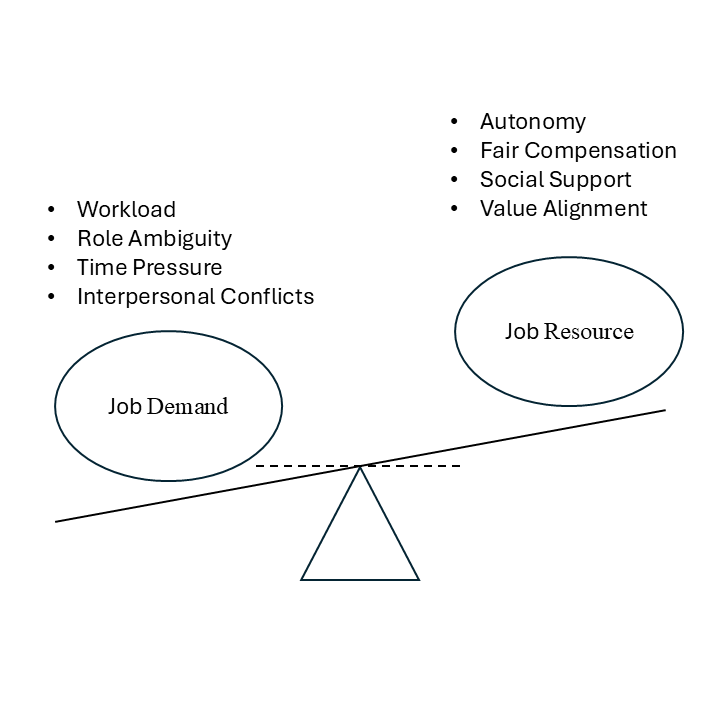
\includegraphics[width=4.16667in,height=\textheight,keepaspectratio]{Figure.png}
\caption{Imbalance in Job Demand and Resources (JD-R Model)}
\end{figure}

Maslach and Leiter (2016) present a conceptual framework of burnout
syndrome aligned with the Job Demands--Resources (JD-R) model (see
Figure 1). In this model, burnout arises when job demands exceed
occupational resources available to employees. Accumulated occupational
stress is typically associated with work overload, lack of autonomy, and
ambiguity of roles. Workload refers to the extent to which assigned
tasks deplete capacity of employees in the workplace. Excessive working
hours, as a quantifiable form of workload, are frequently associated
with both physical and mental health problems that are closely linked to
burnout (Jung \& Kim, 2021; Edú-Valsania et al., 2022; J. Kim et al.,
2024).\footnote{Aligning with behavior consequences, Edú-Valsania et
  al.~(2022) reviewed that burnout exposure can be represented as
  accumulated stress, absenteeism, presenteeism with less productive
  outcomes, and fatigue. In psychological terms, Jung \& Kim (2021)
  argue that excessive working hours result in depression with
  data-driven evidence in Korea. J. Kim et al.~(2024) also claims risk
  of suicide caused by long working hours from analysis in Korea.}
Existing literature identifies psychological, health-related,
behavioral, and organizational consequences of burnout (Maslach \&
Leiter, 2016; Edú-Valsania et al., 2022). As one of the direct
behavioral outcomes, job dissatisfaction serves as an empirical proxy,
linking previous studies in psychology and labor economics.

Job satisfaction or life satisfaction is widely used as a proxy for
individual utility in applied microeconomics. As a foundational
proposition, Freeman(1978) suggests that self-evaluations of job
satisfaction may contain indirect information regarding individual
utility in the workplace, particularly by reflecting turnover
intentions. However, it is imperative to clarify how previous studies
handled its controversial nature, which arises from defining and
standardizing the empirical measurement of utility. Winkelmann \&
Winkelmann (1998) demonstrate that subjective outcome variables can
yield meaningful insights in labor market analysis if anchoring problems
are addressed. Beyond its use on labor force participation, C.Green \&
Heywood (2008) argue that subjective welfare reports contribute to the
analysis of various effects such as performance pay incorporating
objective economic indicators. Additionally, life satisfaction and
subjective mental health reports contribute to analyzing the internal
impact of individuals on the allocation of work and labor productivity
(F.Green, 2011; Oswald et al., 2015).

Multiple studies on job disutility offer insights into burnout (Greiner,
2008; Rätzel, 2012). Rätzel (2012) incorporates the non-pecuniary
components into a utility function, independent of wage or income. The
non-pecuniary property holds an inverse U-shape on both under- and
over-employment. Building upon the labor-leisure tradeoff, Greiner
(2008) examines the impact of work-related stress on utility derived
from consumption and labor. Within this framework, accumulated stress
shapes the marginal disutility of labor over time, arising from long
working hours and work intensity. Aligning with diminishing marginal
utility, the dynamic model between stressors and behavioral consequences
of burnout describes fatigue accumulation and the recovery process
(Jacobs \& Piyapromdee, 2016; Pencavel, 2016b; Donsimoni, 2020). Jacobs
\& Piyapromdee (2016) crystallized how stress exposure impacts
individual entrance or out of the labor force, especially for older
workers. Proper impact on labor supply, distinct from health status, and
high levels of stress reported by workers negatively affect labor force
participation unless the recovery process is held on time. Pencavel
(2016b) argues that an intensive working schedule influences not only
the performance of workers within their exhaustion. Donsimoni (2020)
confirms fatigue negatively impacts labor supply and further suggests a
multiple parameter regarding job sensitivity to stress.

Motivated by previous research, I provide a simplified framework of job
disutility from working hours and labor shortage conditions. Despite
lots of papers proposing life satisfaction as a proxy of utility in a
wide context, I limit job satisfaction as an outcome variable to
maintain commonality in the findings of burnout literature.\footnote{Individual
  welfare change in the long-term through job satisfaction and life
  satisfaction was assessed for causality verification from working hour
  reduction in Korea. Job satisfaction was more instantly impacted by
  policy compared to life satisfaction (see Ko \& Jung, 2023). Also,
  Russo (2012) present a similar trends between job and life
  satisfaction related to utility context.} Based on previous research
on job satisfaction as a variable, aggregated sub-components of job
satisfaction are recommended as a mean value (Rose, 2001; Bae, 2008).
Giving attention to related work on job satisfaction and working hours
in Korea, I additionally contribute to assessing an impact based on
working hour composition on workweek with labor shortage conditions (H.
Kim et al., 2015; J. Kim et al., 2017). Regarding the endogeneity
between working hours and job satisfaction, a recent empirical study
suggests that only independence in overtime work choice had a positive
factor (see Chung et al., 2018).\footnote{Although Chung et al.~(2018)
  tried to verify the statistical significance of overtime work by
  comparing it to normal working hours and general job satisfaction with
  a 1 to 5 Likert scale through OLS with random effect, I differently
  measured outcome. Further discussion is provided in the Estimation
  Method.} By using Ordered Logit with Fixed-Effects, I alternatively
provide probability change in job satisfaction variation on time of
certain individuals who experienced excessive working hours.
Additionally, as Winkelmann \& Winkelmann (1998) point out, I use
ordered logit with fixed effects on units of each random variable to
alleviate anchoring issues by providing within-variation results.
Through incorporating a given theoretical framework and empirical
evidence, this study provide insights into how worker burnout from
overwork can be manifested through the structure of the work
environment.

\newpage

\section{THEORETICAL FRAMEWORK}\label{theoretical-framework}

Presenting framework assumes that burnout is the occupational phenomenon
resulting from the gap where actual working hours are longer and more
intensive than their optimal level. This excess is often driven by labor
shortages in specific markets, which function as external constraints
that push employees to work longer hours irrespective of their own
preferences. In such contexts, working hours affect not only consumption
and leisure trade-offs but also non-pecuniary utility, such as
psychological well-being and fatigue. If working hours are excessive,
workers experience negative utility containing fatigue, detaching
behavior, and the depreciated value of work. Burnout from overwork
occurs precisely when fatigue overrules psychological satisfaction with
a lack of adaptable recovery time. A structured framework would be
empirically testified in the Estimation Method.

\subsection{Labor Shortage as a Market
Constraint}\label{labor-shortage-as-a-market-constraint}

Long working hour issues might reflect production and organizational
constraints in the Korean labor market if direct working hour regulation
does not entirely deconcentrate overtime of certain individuals. Kang \&
Park (2023) argue that the job-sharing effect was limited after the
52-hour regulation in Korea. According to their theoretical
prepositions, reallocation of overtime to additional workers can be
accomplished when substitution effects are more dominant than increasing
the production scale. Regarding determinants of the cases when hiring
new employees is more beneficial than overtime use, Hart (2004) proposes
the comparative advantage in labor costs for new employees and the labor
market where an adequately skilled workforce is sufficiently present.
Despite the strict intervention, the motivation in overtime uses of
employers cannot be fully eliminated without the aforementioned
conditions if the firm maintain the scale of production. As the one of
primal constraints, I suggest labor shortages in the market which still
impact overtime of employees.

\begin{figure}
\centering
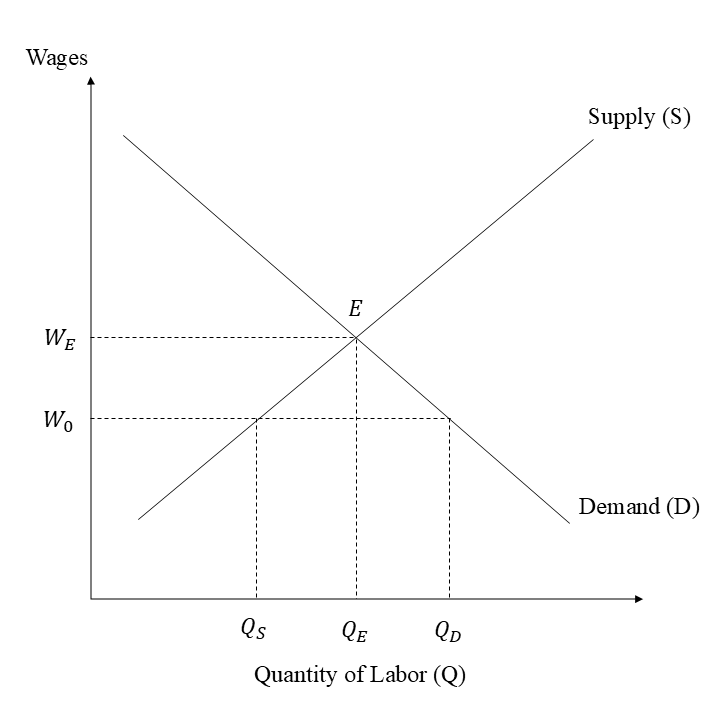
\includegraphics[width=4.16667in,height=\textheight,keepaspectratio]{lbs.png}
\caption{Disequilibrium between Labor Supply and Demand}
\end{figure}

Labor shortages stem from a combination of rising desired living
standards and a shortage of qualified workers for specific industries in
the domestic labor market. The deficit of employees can be summarized as
a misalignment between the market-clearing price of labor (\(W_E\)) and
the actual payable cost of labor (\(W_0\)) where other determinants of
supply and demand hold constant. Figure 2 presents the case where the
cost of employment in a hiring market where participants in the demand
side share the volume and type of production is set below the
equilibrium point.\footnote{The figure is based on the content for the
  social demand model of Chapter 1 in Barnow et al.~(2013).}

Equation 3.1, derived from Figure 2, on the basis that the actual wage
rates (\(W_0\)) are lower than the market clearing price (\(W_E\)),
labor shortages (\(LS_{condition}\)) occur as the quantity of labor
demand, \(Q_D\), is more dominant than the quantity of labor supply,
\(Q_S\). The demand for labor inputs, \(f(X_D)\), is combined with
production factors including the level of productivity, the volume of
capital, and the required skills of labor matching with its
technological progression. Subsequently, the aggregated decisions in
labor force participation, \(g(X_S)\), are also affected by the profiles
and needs of related individuals. On both parts, the elasticity of wage,
\(\alpha\), and \(\beta\) impact on the volume of employment align with
the empirical evidence of Lim \& Lee (2024).\\
\[
LS_{condition}: Q_S(W_0) < Q_D(W_0)\quad if \quad W_0 < W_E, \quad \text{where}
\begin{cases}
Q_D = f(X_D)-\beta W_0 \\
Q_S = g(X_S)+\alpha W_0
\end{cases}
\tag{3.1}
\]

Hence, inadequate wage rates cause workforce shortages relative to the
potential candidates in the corresponding labor market. Slow adjustments
of firms may not successfully fulfill the deficit, especially for
small-sized with a rigid production process. Applying the given
framework to the relative firms, employers can choose overtime as a
coping strategy when the difficulty presents in seeking adequately
skilled workers (Hart, 2004; Barnow et al., 2013). Under the labor
shortage constraint, employers might substitute unfulfilled vacancies
with overtime use of current employees without fixed fringe payments.
Employees accept overtime unless they find alternative occupations for
which they can be instantly hired. As Pencavel (2016a) argues,
individual working hours may not reflect pure self-determined
optimization results considering the aforementioned predominant market
constraints.

\subsection{Optimization of Working Hours and Fatigue-Driven
Burnout}\label{optimization-of-working-hours-and-fatigue-driven-burnout}

\begin{figure}
\centering
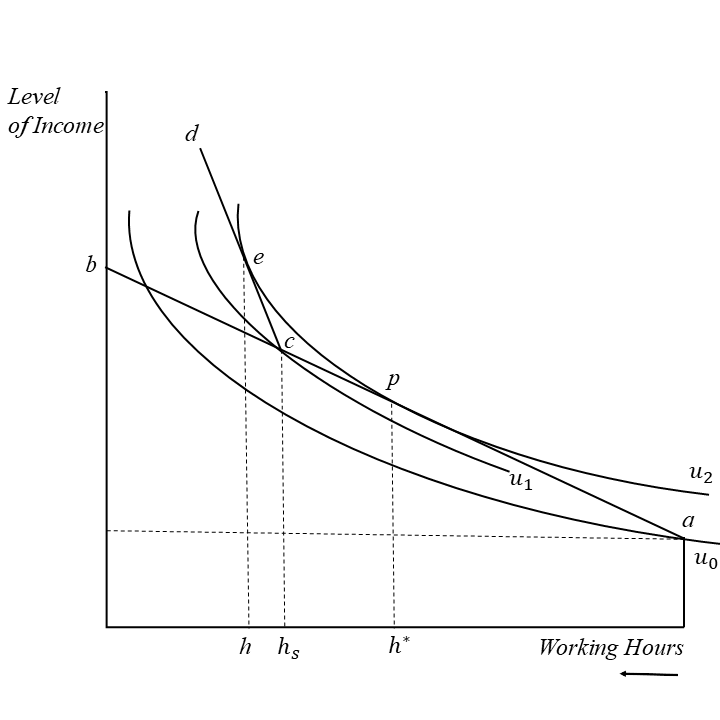
\includegraphics[width=4.16667in,height=\textheight,keepaspectratio]{Individual overwork decision.png}
\caption{Individual Labor--Leisure Trade-off and Overtime Decision}
\end{figure}

Assuming that the indifference curve of individual preference is convex,
Figure 3 shows how individuals decide on optimal working hours
\(h^*\).\footnote{The figure is based on the content of chapter 3 in
  Hart (2004).} If real wage (\(wh\)) is equal to the slope (\(a-b\))
starting from the point (\(a\)) representing non-labor income (\(V\)),
the optimal working hour of an individual is equal to the point \(h^*\)
where the marginal substitution rate of consumption (\(C\)) and leisure
(\(L\)) is identical with wage rates (\(w\)).

In response to the needs of firms for overtime allocation, Hart (2004)
proposes cases on the supply side accept overtime work. First, the
labor-leisure trade-off assumes that individual working motivation
corresponds to the maximized utility under budget constraints. As
Equation 3.2 presents, Individuals seek the optimal level of working
hours (\(H^*\)) on maximized utility points incorporating the bundle of
consumption (\(C\)) and leisure (\(L\)). Taking account of the suggested
bundle, the level of consumption (\(C\)) is approximately identical to
the level of income (\(I\)) without saving. Individual income (\(I\)) is
equal to the sum of labor income (\(wH\)) and non-labor income (\(V\)).
Labor income (\(wH\)) is represented as the combination of wage rate
(\(w\)) and participated volume of work (\(H\)). Besides individual
consumption, as another component of the bundle, leisure (\(L\)) can be
represented as the rest of the working hours in the entire disposable
time (\(T-H\)). If the preference bundle satisfies complete and
transitivity on each element \(C\) and \(L\), the utility function of
the individual is validated in approaching labor market analysis. The
optimal level of working hours (\(H^*\)) exists if the disposable level
of consumption (\(wH+V\)) and leisure (\(T-H\)) of individuals can be
optimized at a certain point of \(H\). \[
\begin{aligned}
H^*
&= U(C,L) \\
&= \arg\max_H U(wH+V,T-H)
\end{aligned}
\tag{3.2}
\]

Two cases are derived from Figure 3, based on Equation 3.2. Comparing
both cases serves to clarify the variation of preferences when overtime
work is accepted by individuals.

In the first case, firms provide the overtime premium (\(d-c\)),
adjusted to the normal wage rates (\(a-b\)).\footnote{The figure is
  based on the content of chapter 3 in Hart (2004).} Overtime worker
accepts working hours change from \(h^*\) to \(h\) on the same level of
utility, \(u_2\). Compare to the slope \(a-b\) which is equal to
\(wH+V\), it is imposed on \(H\) where exceed \(h_s\) as
\(w_{OT} = w(1+r), r > 0\) instead of \(w\). \[
u_2 \approx u^* : U(w_{OT} \cdot h_s + v, T-h_s) = U(wh^*+V,T-h^*)
\tag{Case 1}
\]

In the second case, assume that working more as \(h_s - h^*\), which is
not fully compensated by overtime payment, with almost indifferent
between \(w\) and \(w_{OT}\) at individual perception. Workers
experience a diminishing utility from \(u_2\) to \(u_1\). Since the gap
\(u_2-u_1\) is greater, such work-adverse behavior (e.g., absenteeism)
might have originated in the worker group. If \(u_1 \succ u_0\) holds,
the individual does not decide to exit from the current occupation. \[
u^* \succ u_1 : h_s - h^* > 0,\quad \text{with } w_{OT} \approx w 
\tag{Case 2}
\]

However, the remaining workplace of individuals accepting overtime does
not fully imply that the level of individual utility holds as \(u_2\) or
workers assume \(u_1 \succ u_0\) because employees are affected by their
loyalty and slow adjustment. Also, the level of compensation does not
fully substitute the loss induced by long working hours such as
individual welfare or health. Elaborating on the assumption of utility
loss due to long working hours, Rätzel (2012) proposes an uncharted part
in the individual labor supply decision. The suggestion of a pure
motivation to participate in work without monetary compensation provides
how individuals avoid unemployment if the volume of work is not too
excessive. Conversely, negative outcomes such as stress, fatigue, and
also burnout can be induced by excessive working hours notwithstanding
wage compensation. So the author suggests non-pecuniary utility,
containing marginal variation in working hours, as \(N(H)\) adjusted in
Equation 3.3 from Equation 3.2. \[
H^* = U(C,L) +N(H), \quad N'(H)>0, \quad N''(H)<0
\tag{3.3}
\]

If an individual decides on working hours (\(H^*\)) only based on
\(U(\cdot)\), the level of utility would be monotonically increased by
consumption (\(wH+V\)) and leisure (\(T-H\)). Hence, the constant
curvature of the function \(U(\cdot)\) derives the optimized point
(\(H^*\)) with a marginally diminishing pattern. However, if the
individual also depends on non-pecuniary utility \(N(\cdot)\), the
relation between working hours (\(H\)) and individual utility (\(U\))
might exhibit a negative and steeper slope on the range of excessive
working hours. Through the aggregate utility function, it is possible to
ratiocinate how individual preference fluctuates based on the
distribution of working hours (\(dF(H)\)). \footnote{The expected
  aggregate utility curve plotted in Figure 4 is based on the following
  stylized expression:
  \(\mathbb{E}[U_{\text{agg}}] = \int_h \left[ \mathbb{E}_{i,t} \left[ U(w_{it} H + v_{it},\ T - H) + N(H) \,\middle|\, H_{it} = H \right] \right] dF(h)\).
  Although the following expression is not used for estimation, it
  provides a theoretical illustration of how aggregate preferences
  fluctuate over the distribution of working hours.} The conditional
expected utility (\(\mathbb{E}[U_{\text{agg}}]\)) on weekly working
hours (\(H\)) of individuals(\(i\)) at the observed time (\(t\)) shows
how the level of job satisfaction is estimated on average.

\begin{figure}
\centering
\pandocbounded{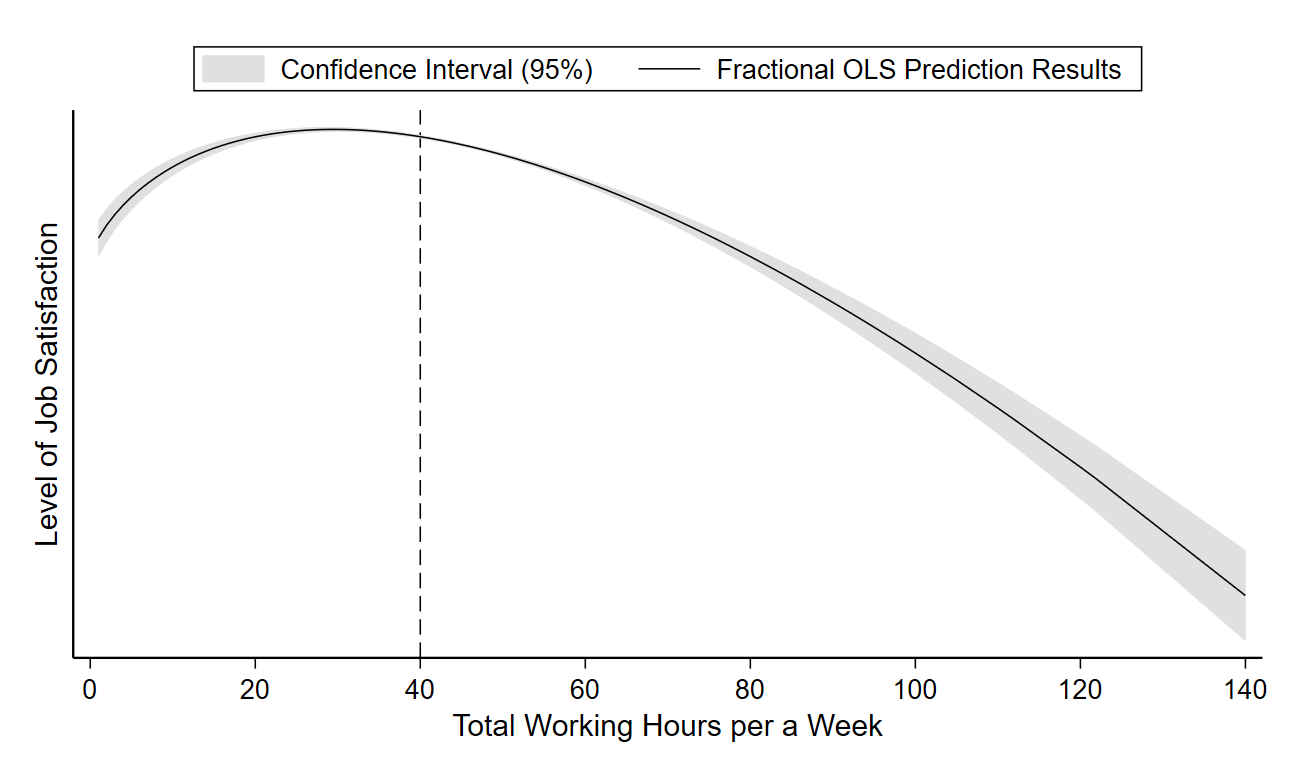
\includegraphics[keepaspectratio]{images/Graph_working hour(week).png}}
\caption{Aggregated Job Satisfaction by Weekly Working Hours}
\end{figure}

Figure 4 presents the relationship between weekly working hours and job
satisfaction with an inverse U-shape.\footnote{Aggregating individual
  utility on working hours is visualized by the data presented in this
  paper. Using fractional polynomial regression,
  \(H^{(p1, p2, ..., pm)} \beta'\), applied to KLIPS data. The job
  satisfaction index combines both pecuniary and non-pecuniary
  components. Standard errors are calculated through the clustering of
  each individual. Further information on data is provided in the
  following chapters.} The concave relation shows that the maximized
level of job satisfaction reaches nearly 30 and 35 hours and slightly
decreases until 40 hours as Hart (2004) argues regarding overtime
premium. The overtime workers achieve a lower level of job satisfaction
with a steeper diminishing pattern according to the provided empirical
estimation. This pattern supports the argument of Rätzel (2012) that the
disutility from long working hours eventually outweighs the gains from
monetary compensation. Focusing on a gradually negative slope after the
threshold of regular working hours (40 hours per week), increasing
fatigue with longer working hours can be expected in the following
analysis. As Winkelmann \& Winkelmann (1998) emphasized, this
demonstrated relationship should be noted within the limitation that
individual perception is not homogeneous.

While Rätzel (2012) generally incorporates the aspect of psychological
well-being, non-pecuniary utility (\(N(H)\)), recent studies disentangle
its negative component by explicitly modeling intrinsic fatigue as a
separate function of working time (\(F(H)\)) with particular attention
to recovery constraints as Equation 3.4 (Jacobs \& Piyapromdee, 2016;
Pencavel, 2016b; Donsimoni, 2020). Jacobs \& Piyapromdee (2016) estimate
reduced labor force participation of individuals in occupational
exhaustion based on preference parameters and the burnout-recovery
process. In addition to the time of recovery, Pencavel (2016b) claims
that excessive working hours without necessary restoration result in
work performance loss\footnote{Although work performance is not
  conceptually identical to individual disutility, both are considered
  symptomatic outcomes of burnout (Maslach \& Leiter, 2016; Edú-Valsania
  et al., 2022). Also, the assumption that lack of recovery within long
  working hours results in negative effects is adaptable to the
  mechanism of burnout.} by the assessment with dummy variables such as
whether an individual worked on Sunday and the lagged hours worked
during the previous work weeks. Donsimoni (2020) conceptualizes utility
loss from occupational fatigue as an exposure to stressful tasks at work
that strains individual utility maximization. Based on these insights, I
formulate the non-pecuniary utility (\(N(H)\)) as the psychological
satisfaction derived from work (\(M(H)\)), offset by occupational
fatigue (\(F(H)\)). Both parameters depend on the allocated time with
recovery opportunities. \[
N(H) = M(H) - F(H)
\tag{3.4}
\]

On the premise that \(M(H)\) is the positive baseline of \(N(H)\), the
function of fatigue on working hours \(F(H)\) is structured through
Equation 3.5 with the following sub-components of total working hours
(\(H\)): Average working hours per day (\(\bar{h}\)) and days of work
per week (\(d\)). As argued by Pencavel (2016b), the immediate benefits
of shorter hours per day and shorter working weeks are considered in the
bundle of working schedules (\(H\)). The trade-off between working hours
and time of rest is incorporated concerning the burnout-recovery process
(Jacobs \& Piyapromdee, 2016; Donsimoni, 2020). Even if the total
working hours (\(H\)) among workers are identical, its composition will
differ individual fatigue inducement since the elasticity (\(\gamma\)
and \(\delta\)) and the effects (\(\theta_1\) and \(\theta_2\)) of each
component are distinctive and positive. Accordingly, the presented
specification in Equation 3.5 would supplement how the psychological
disutility of workers is conceptualized. \[
\begin{aligned}
F(H)
&=F(\bar{h}, d) \\
&= \theta_1 \cdot \left( \frac{1}{24-\bar{h}+\epsilon} \right)^\gamma + \theta_2 \cdot \left(\frac{1}{7-d+\epsilon}\right)^\delta
, \quad \text{where } H = \bar{h} \cdot d, \quad \gamma>0, \quad \delta>0
\end{aligned}
\tag{3.5}
\]

This chapter has established a theoretical model in which excessive
working hours, induced by market-level labor shortages, lead to job
disutility and potential burnout through the accumulation of fatigue.
Equation 3.1 describes a market disequilibrium that generates labor
shortages, which externally constrain the internal optimization of labor
supply and demand. In response, when employers allocate overtime to
existing employees, Equation 3.2 distinguishes two possible outcomes
based on the classical labor-leisure trade-off and preliminary
optimization of working hours: either accepting overtime with no utility
loss or accepting it with diminished satisfaction but without exiting
the labor force. An unchanged level of utility implies that incentives
compensate for the marginal disutility of additional work. In contrast,
diminished utility without full withdrawal reflects involuntary labor
participation under rigid market conditions, such as delayed
occupational transition. Equation 3.3 formalizes how non-pecuniary
utility varies even when wage compensation exists. This utility can be
decomposed, as shown in Equation 3.4, into two parameters: psychological
satisfaction derived from the job, and the negative offset caused by
occupational fatigue. Assuming a concave relationship between working
hours and utility due to these opposing forces, Equation 3.5
incorporates the role of recovery opportunities within finite time.
Altogether, this framework provides a foundation for empirically
analyzing how excessive working hours, imposed by structural labor
market constraints, impact individual well-being. The subsequent chapter
tests these mechanisms by examining how labor shortages shape working
time and, in turn, influence job satisfaction.

\newpage

\section{ESTIMATION METHOD}\label{estimation-method}

\begin{figure}
\centering
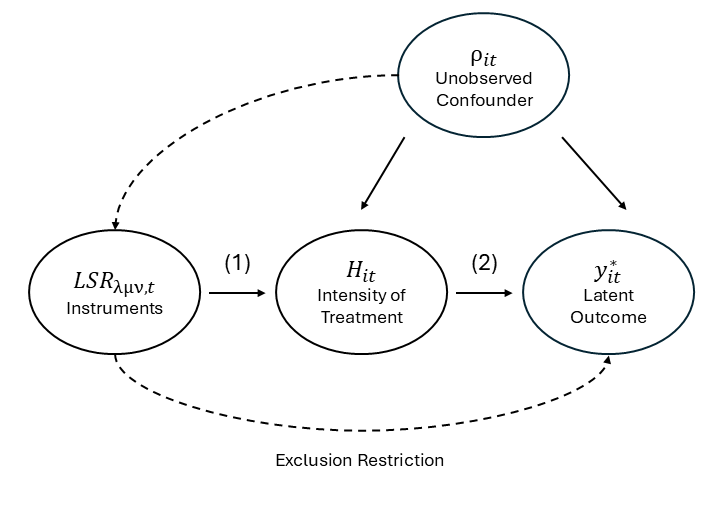
\includegraphics[width=5.20833in,height=\textheight,keepaspectratio]{DAG.png}
\caption{Directed Acyclic Graph of Instrumental Identification}
\end{figure}

This study investigates how structural labor market constraints causally
contribute to individual burnout. Burnout is conceptualized as a
deviation from optimal labor-leisure allocation due to involuntary
overtime. Figure 5 shows a directed acyclic graph (DAG) that illustrates
a two-stage causal mechanism identified in the empirical model using an
Instrumental Variable (IV) approach. The first baseline estimation
assesses whether labor shortage across industries influences the working
hours of employed individuals. Subsequently, I examine the negative
effects of working hours on individual job satisfaction, a key domain of
utility in a work-related context. Finally, the estimated causal effect,
using 2SPS under the Average Causal Response (ACR) theorem, demonstrates
that individual long working hours affected by labor shortage reduce the
probability of achieving utility maximization. To ensure the robustness
of 2SPS estimation, the following key assumptions are validated:
Relevance, exclusion restriction, and monotonicity. In contrast to
previous studies that argue the relationship between long working hours
and individual hazards has reverse causality (e.g., presenteeism), this
paper provides partial evidence that the volume of additional and
involuntary working hours marginally increases the probability of
burnout in a given period due to inevitable overtime (see Jung \& Kim,
2021). Additionally, identifying involuntary working hours in the
burnout framework is necessary for empirical assessment due to
confounders in individual working hour determination regarding the
incentive of overtime (Hart, 2004; Park \& Park, 2019; Lim \& Lee,
2024).

\subsection{Two-Stage Baseline Estimation: Working Hours and Job
Satisfaction}\label{two-stage-baseline-estimation-working-hours-and-job-satisfaction}

Using Equation 3.1, I can rewrite a function on labor force
participation change of employed individuals. I only investigate
employed individuals by firms to testify if a lack of workforce in the
labor market relates to an increase in individual working hours. The
projected increase in occupational demand is measured to indicate how
establishments are affected by the shortage of workforce in the present
market. Its condition is approximately defined as a reported sum of
establishments where 16 industrial categories (\(\lambda\)), 5
categories of firm size (\(\mu\)), and 17 regions (\(\nu\)) are common
on a given period (\(t\)). It is constructed by aggregating the number
of job vacancies and current employees in establishments that fall under
the same \(\lambda\mu\nu\) combination, and averaging the
vacancy-to-position ratio within each segment: \[
\text{LSR}_{\lambda\mu\nu,t} =  \frac{\text{Vacancy}_{\lambda\mu\nu,t}}{\text{Current}_{\lambda\mu\nu,t}+\text{Vacancy}_{\lambda\mu\nu,t}}\times 100, \quad t \in \{1, \dots, T\} 
\]

The first stage of estimation alternately estimates the impact of labor
market constraints using industrial labor shortage clusters, aiming to
provide industrial heterogeneity over time, alongside its between- and
within-variation. Clusters are structured through industry-level time
series that aggregate over firm size and region. In practice,
\(LSR_{\lambda,t}\) already incorporates the internal distribution of
firm size and regional composition within each industry through a
weighted calculation by the Ministry of Employment and Labor. \[
\text{LSR}_{\lambda,t} = \frac{1}{|\mu| \cdot |\nu|} \sum_\mu \sum_\nu \text{LSR}_{\lambda\mu\nu,t} := \text{Avg}_{\mu,\nu}\left( \text{LSR}_{\lambda\mu\nu,t} \right)
\]

This aggregation yields a time series vector of labor shortage rates for
each industry \(\lambda\), capturing the evolution of structural labor
market conditions over the observed period. Each vector
\(\mathbf{LSR}_\lambda\) represents the sequence of yearly shortage
rates from 2009 to 2023 and serves as the fundamental input for the
clustering procedure: \[
\mathbf{LSR}_\lambda = \left( \text{LSR}_{\lambda,1}, \text{LSR}_{\lambda,2}, \dots, \text{LSR}_{\lambda,T} \right) \in \mathbb{R}^T
\]

The clustering procedure simplifies the analysis by grouping industries
with similar labor shortage patterns over time. The distinction among
clusters was based on the Euclidean norm of their respective labor
shortage vectors. The distance between industries \(\lambda\) and
\(\lambda'\), using Euclidean norm of their respective vectors
\(\mathbf{LSR}_\lambda\), is computed as follows: \[
d\left( \lambda, \lambda' \right) = \| \mathbf{LSR}_\lambda - \mathbf{LSR}_{\lambda'} \| = \sqrt{ \sum_{t=1}^{T} \left( \text{LSR}_{\lambda,t} - \text{LSR}_{\lambda',t} \right)^2 }
\]

Given these pairwise Euclidean distances of each industry \(\lambda\)
and \(\lambda'\), hierarchical clustering is conducted using Ward's
minimum variance method. The minimized increase in the total
within-cluster sum of squared errors (SSE), denoted by \(\Delta_{ij}\),
determines the cost of merging two clusters \(C_i\) and \(C_j\). \[
\Delta_{ij}=\frac{|C_i||C_j|}{|C_i| + |C_j|} \cdot \| \mathbf{\bar{LSR}}_{Ci} - \mathbf{\bar{LSR}}_{Cj} \|^2
\]

Here, \(\mathbf{LSR}_C\) denotes the average labor shortage vector of
industries within each cluster \(C_k\). The optimal clustering structure
is obtained by minimizing the total within-cluster variance across all
clusters (see Figure 6; see also Figures A1 and A2): \[
\min_{\{C_k\}} \sum_{k=1}^{K} \sum_{\lambda \in C_k} \left\| \mathbf{LSR}_\lambda - \bar{\mathbf{LSR}}_{C_k} \right\|^2
\]

To examine whether labor shortage rates affect working hour decisions, I
define the outcome vector \(\mathbf{H}_{it}\) to include four components
derived from Equation 3.2. First, its impact on working
hours(\(H_{it}\)) variation from the total available time (\(T\)) per
week is comprised. Subsequently, I break down weekly working hours
(\(H_{it}\)) into two main components of average working hours per day,
\(\bar{h}_{it}\), and actual working days per week, \(d_{it}\), to
testify if dominating labor shortages in engaged market impact not only
the volume of total working hours (\(H\)) but also its composition.
Linear probability on overtime participation
(\(\mathbf{1}\{H_{it} > 40\}\)) is additionally assessed to simply
investigate whether workers participate in overtime work due to the
shock. \[
\mathbf{H}_{it} \in \{H_{it}, \bar{h}_{it}, d_{it}, \mathbf{1}\{H_{it} > 40\} \}
\]

Equations of the first stage represent a reduced-form hybrid hours-wages
equation, inspired by the identification problem raised in Pencavel
(2016a). By incorporating labor shortage rates into the primal working
hours equation, it shows how labor shortages, which reflect both labor
supply and demand constraints formulated by Equation 3.1, impact
individual working hours beyond the preference-based labor supply
assumption. The model estimates whether labor shortage leads to longer
working hours among incumbent workers, employing individual fixed
effects (\(\alpha_i\)) to control for unobserved heterogeneity. It also
controls categories of job (\(\delta\)), and each unit of labor shortage
rate: industrial categories (\(\lambda\)), categories of firm size
(\(\mu\)), and regions (\(\nu\)). The control vector \(Z\) comprises the
factors related to \(U(wh+V)\) as specified in Equation 3.2, such as
wage rates(\(w\)), paid vacation offerings classified as a part of a
compensation package, and monthly income of the household (\(V\)). To
avoid the omitted variable bias, \(Z\) includes household
characteristics (e.g., number of household members and marital status),
as well as variables related to working conditions and employee
profiles, such as ages, years of tenure, and type of contracts including
atypical, temporary, or public employer (see Appendix Table A1).

To support Equation 4.1, Equation 4.1 provides a basic estimation of
continuous labor shortage rates to derive effects on individual working
hour vectors. Baseline to Equation 4.1, the following auxiliary model
presents the general effects of labor shortage rates on individuals. \[
\mathbf{H}_{it}=\beta_0 + \beta_1 \text{LSR}_{\lambda\mu\nu,t} + Z_{it}' \gamma + \delta_{it} + \lambda_{it} + \mu_{it} + \nu_{it} +\alpha_i + \epsilon_{it}
\tag{4.1}
\]

Through the derived hierarchical clusters, denoted by
\(g_{\lambda(i,t)} \in \{1,2,3,4\}\), Equation 4.2 extends the
specification in Equation 4.1 by replacing the continuous labor shortage
rate with industry-level ordinal cluster dummies. Cluster assignments
are used to compare the between-variation of labor shortage rates among
industrial clusters. Cluster 1 serves as the reference category
corresponding to the lowest structural labor shortage. \[
\mathbf{H}_{it} = \beta_0 + \sum_{c=2}^{4} \beta_c \cdot \mathbf{1}\{g_{\lambda(i,t)} = c\} + Z_{it}' \gamma + \delta_{it} + \mu_{it} + \nu_{it} + \alpha_i + \epsilon_{it},
\quad \text{with } \beta_1 = 0
\tag{4.2}
\] To show how a clustered variation in labor shortage rates impacts
individual working hour decisions, Equation 4.1 estimates the with-in
slope of labor supply responses by interacting labor shortage rates with
cluster dummies. The variable \(g_{\lambda(i,t)}\) indicates the cluster
group \(c\) of the industry \(\lambda\) in which individual \(i\) is
employed at time \(t\). Predicted results from Equation 4.1 substitute
observed working hours for IV estimation. Although the responsiveness of
workers in Cluster 1 is expected to be inactive, its inclusion allows
for identifying the relevance of labor shortage rates in the working
hour decision across all industry groups and unmeasured confounders in
further stages. \[
\mathbf{H}_{it} = \beta_0 + \sum_{c=1}^{4} \beta_c \cdot \left(\mathbf{1}\{g_{\lambda(i,t)} = c\} \cdot \text{LSR}_{\lambda\mu\nu,t} \right) + Z_{it}' \gamma + \delta_{it} + \mu_{it} + \nu_{it} + \alpha_i + \epsilon_{it}
\tag{4.3}
\]

The first stage of estimation contributes to indicate the limitation
where previous literature assumes that the actual working hours are
decided by the pure optimization process. The gap between desired
working hours (\(H^*\)) and actual working hours (\(H\)) not only
resulted from individual conditions but also from the unfulfilled
demands of the workforce in the labor market. The overtime pressure
shaped by labor shortage provides partial grounds for how individuals
are dissatisfied with excessive working hours at subsequent equations in
estimation.

From Equation 3.3, provided in Theoretical Framework, I verify if
excessive working hours negatively impact the job satisfaction of
employees while controlling the wage rate. Due to the ordinary
measurement of satisfaction on the Job Descriptive Index (JDI) with 5
Likert scales, it is imperative to use ordered logit instead of OLS as
mentioned in Literature Review. In the outcome variable, I include two
related domains to pecuniary utility, such as wage and working hours,
and the other three domains in non-pecuniary utility: the value of work,
working environment, and quality of communication. The composite outcome
of five sub-factors is derived from the process as below. \[
y_{it} =  \frac{1}{5} \sum_{k=1}^{5} JS_{it}^{(k)}, \quad i \in \{1, \dots, N\}, \quad t \in \{1, \dots, T\}
\]

Since the dependent variable (\(y_{it}\)) is equal to the mean value of
5 ordinal variables in each facet measurement of job satisfaction, it
needs to be transformed as the latent outcome (\(y^*_{it}\)), altered
with respect to the continuous property. Since the difference between
the responses \emph{`Very satisfied (5)'} and \emph{`Generally satisfied
(4)'} can not be concluded as the same between \emph{`Generally
satisfied (4)'} and \emph{`Neutral (3)'}, the observed outcome
\(y_{it} \in \{1, \dots 5\}\) is then defined as a dichotomy of
\(y^*_{it}\) based on cut-points \(\{\tau_k\}_{k=1}^{20}\). The given
thresholds (\(\tau\)) segment latent space of \(y^*_{it}\) into
intervals corresponding to the composite set of Likert scales. So, the
magnitude of each explanatory variable on the total effect is measured
as the change of probability among intervals in logistic distribution.
\[
y_{it} =
\begin{cases}
1, & y^*_{it} \leq \tau_1 \\
\vdots & \vdots \\
3, & \tau_{10} \leq y^*_{it} \leq \tau_{11} \\
\vdots & \vdots \\
5, & \tau_{20} \leq y^*_{it}
\end{cases}\quad
\text{where } \{\tau_1, \dots, \tau_{20}\}
\]

To show the impact of working hours on job satisfaction, I empirically
rewrite Equation 3.3 under the assumption that the gap between \(H-H^*\)
creates a negative magnitude itself. Identically as shown in the first
stage, vector \(Z\) implies household characteristics (e.g., number of
household members, marital status, and monthly income of the household)
and other variables related to working conditions, and profile of
employees such as ages, wage rates, paid vacation offer, years of tenure
and type of contracts (including atypical, temporary or public
employer). Three categories of job (\(\delta\)) and each variable
regarding Equation 4.1, such as industrial categories (\(\lambda\)),
categories of firm size (\(\mu\)), and regions categories (\(\nu\)) are
also controlled. \[
y^*_{it} = \phi(H_{it}) + Z_{it}' \gamma + \delta_{it} + \lambda_{it} + \mu_{it} + \nu_{it} +\alpha_i + \epsilon_{it}
\tag{4.4}
\]

Through decomposing \(\phi(H_{it})\), which holds the function of
working hours, in Equation 4.2, it is possible to verify both linear and
non-linear cases. It follows the case provided by Rätzel (2012), inverse
U-shape while controlling wages. \[
\phi(H_{it}) =
\begin{cases} 
\beta_1 H_{it} & \text{(Linear Format)} \\
\beta_1 H_{it} + \beta_2 H_{it}^2 & \text{(Quadratic Format)}
\end{cases}
\]

Following the theoretical framework in Equations 3.4 and 3.5,
conceptualized occupational fatigue from the burnout-recovery process, I
designed the auxiliary model, Equation 4.2a. The suggested equation
decomposes total working hours into two parameters, average hours per
day (\(\bar{h}\)) and number of workdays (\(d\)) per week. It assesses
which dimension of labor time configuration is more decisive on marginal
disutility between work intensity within a single day and the extended
distribution of work across the week. \[
\phi(\bar{h}_{it} , d_{it}) =
\begin{cases} 
\beta_1 \bar{h}_{it} + \beta_2 d_{it} & \text{(Pure Linear Format)} \\
\beta_1 \bar{h}_{it} + \beta_2 d_{it} + \beta_3 \bar{h}_{it}^2 & \text{(Nonlinear in Daily Hours)} \\
\beta_1 \bar{h}_{it} + \beta_2 d_{it} + \beta_4 d_{it}^2 & \text{(Nonlinear in Workdays)} \\
\beta_1 \bar{h}_{it} + \beta_2 d_{it}+ \beta_3 \bar{h}_{it}^2+ \beta_4 d_{it}^2 & \text{(Fully Quadratic Format)}
\end{cases}
\]

Decomposing \(\phi(\bar{h}_{it}, d_{it})\) in Equation 4.4a incorporates
linear and non-linear cases of total working hours \(H\) into average
working hours per day (\(\bar{h}_{it}\)) and working days per week
(\(d_{it}\)). Here, elasticity (\(\gamma\) and \(\delta\)) and effect
(\(\theta_1\) and \(\theta_2\)) of each component defined as Equation
3.5 are substituted with non-linear formulation and its magnitude from
\(\beta_1\) to \(\beta_4\). A simple comparison between the effect size
of \(\bar{h}_{it}\) and \(d_{it}\) determines a more dominant parameter
on a given workweek allocation. \[
y^*_{it} = \phi(\bar{h}_{it} , d_{it}) + Z_{it}' \gamma + \delta_{it} + \lambda_{it} + \mu_{it} + \nu_{it} +\alpha_i + \epsilon_{it}
\tag{4.4a}
\]

Equation 4.5 expands Equation 4.4 to verify an additional marginal
effect of working hours based on the threshold of overtime work, forty
hours per week, \(\mathbf{1}\{H_{it} > 40\}\). \[
y^*_{it} = \theta(H_{it} \cdot \mathbf{1}\{H_{it} > 40\}) + \phi(H_{it}) + Z_{it}' \gamma + \delta_{it} + \lambda_{it} + \mu_{it} + \nu_{it} +\alpha_i + \epsilon_{it}
\tag{4.5}
\]

Expanding from the auxiliary model, Equation 4.4a, Equation 4.5a allows
measuring the composition effect as an approximate estimation of the
fatigue effect. It operates as a parameter-based model to assess greater
adverse exposure due to the lack of recovery for overtime workers. \[
y^*_{it} = \theta((\bar{h}_{it}, d_{it}) \cdot \mathbf{1}\{H_{it} > 40\}) + \phi(\bar{h}_{it} , d_{it}) + Z_{it}' \gamma + \delta_{it}+ \lambda_{it} + \mu_{it} + \nu_{it} +\alpha_i + \epsilon_{it}
\tag{4.5a}
\]

Estimation from Equation 4.4 to 4.5a structures the burnout process
induced by long working hours. Since Equation 4.1 testifies whether
employees are affected by external constraints on their additional labor
force participation, suggested equations estimate the size of disutility
originated by working hour composition. The concave property of total
working hours (\(H\)) on a given workweek without the compensation
effect proposes a negative hike in non-pecuniary utility after a certain
point of working hours. Equations 4.4a and 4.5a serve as auxiliary
decompositions of total working time aiming at the implication of a lack
of rest within the allocated workweek combination.

\subsection{IV-Based Odds Estimation under the ACR
Theorem}\label{iv-based-odds-estimation-under-the-acr-theorem}

This paper examines the causal impact of long working hours on burnout
using a two-stage Instrumental Variable (IV) method within a logistic
model. Basu et al.~(2018) claim that previous literature has considered
biased estimates of the Average Treatment Effects (ATE) by comparing Two
Stages Predictor Substitution (2SPS) and Two Stages Residual Inclusion
(2SRI) in a non-linear model. Through Monte Carlo simulations, the
authors demonstrate that 2SPS yields consistent and robust estimates of
the LATE even under rare outcome conditions. Consistent with this
condition, this study adopts 2SPS as the main estimation strategy, as
low job satisfaction responses are disproportionately rare and
concentrated at the neutral midpoint (see Table A3). Since working hours
induced by labor shortage rates are translated as the intensity of
treatment, I follow the Average Causal Response (ACR) theorem suggested
by Angrist \& Imbens (1995), instead of the LATE framework. The odds
ratio from 2SPS in a non-linear model can be interpreted as the
Population Odds ratio (POR) under the assumptions of Burgess (2013).

While respecting the Stable Unit Treatment Values Assumption (SUTVA),
Angrist \& Imbens (1995) further present an interpretation of both
multi-valued treatments and counterfactual treatment status under the
ACR theorem. This framework enables the identification of nonlinear
causal relations over working hour distribution by applying the weight
function \(\omega(\cdot)\), derived from the Wald estimator. Compliance
can be testified by comparing the cumulative distribution functions
(CDFs) of the potential treatment intensities induced by the instrument:
\(\mathbf{H}_{1i}\) under treatment and \(\mathbf{H}_{0i}\) otherwise.
Accordingly, I define the average unit causal effect from the intensity
of working hour (\(\bar{H}\)) as follows: \[
\text{ACR} = \int_{0}^{\bar{H}}\omega(H)\cdot\mathbb{E}[\frac{\partial{Y}}{\partial{H}} \mid \mathbf{H}_{1,it} \geq H> \mathbf{H}_{0,it}]dH
\]

Clarifying the composition of the weight function serves to identify the
share of compliers and the validity of the instrument. The structure of
the function equals the size of a group of compliers at point \(H\),
denominated by the mean of the non-negative random variable for the
normalization. The \(\omega(H)\) are non-negative and sum to 1. \[
\omega(H)=\frac{Pr[\mathbf{H}_{1,it} \geq H >\mathbf{H}_{0,it}]}{\int_{0}^{\bar{H}}Pr[\mathbf{H}_{1,it} \geq j >\mathbf{H}_{0,it}]dj}
\]

Following Burgess (2013), I interpret the IV estimate as the odds ratio
conditional on the instrumental strata (i.e., levels of labor shortage),
but marginal with respect to all other covariates, as the ACR theorem
holds. While conventional logistic regression yields a Conditional Odds
Ratio (COR) that is subject-specific and conditional on observed
covariates, the IV-based odds ratio approximates the Population Odds
Ratio (POR), representing a population-averaged causal effect of an
intervention on long working hours. In summary, presenting POR under the
ACR theorem on latent outcome interprets the causal effects based on the
assumption of a weighted average of per-unit average working hours
treatment.

The latent variable \(y^*_{it}\) follows the logistic Cumulative
Distribution Function (CDF). In estimating the probability of the
dependent variable being classified in a particular category, the CDF of
residuals \(\epsilon_{it}\) is assumed to follow a logistic
distribution, \(\Lambda(\cdot)\). To satisfy identification conditions,
\(\epsilon_{it}\) is assumed to be independent of \(X_{it}\) and
\(\alpha_i\) as below. \[
F(\epsilon_{it}| X_{it}, \alpha_i) = F(\epsilon_{it}) =\frac{1}{1 + \exp(-\epsilon_{it})} =\Lambda(\epsilon_{it})
\]

Muris (2017) introduces the Conditional Maximum Likelihood (CML)
estimator for fixed-effects ordered logit models, where the observed
ordered outcome \(y_{it}\) takes value \(k\), conditional on the
individual heterogeneity \(\alpha_i\) and covariates vector \(X_i\). The
CML estimator allows finding a specific probability of \(y^*_{it}\)
between two thresholds \(\tau_k\) and \(\tau_{k+1}\) within a unit of
observation \(i\). \[
Pr\left(y_{it}=k|X_{it},\alpha_i \right)=\Lambda(\tau_{ik+1}-X'_{it}\beta-\alpha_i)-\Lambda(\tau_{ik}-X'_{it}\beta-\alpha_i)
\]

The CML estimates incorporated coefficient \(\beta\) from a dichotomized
ordered variable at each cut-off point. Baetschmann et al.~(2020)
propose Blow-Up and Cluster (BUC) which extends the CML approach by
replicating each observation \(K-1\) times to improve inefficient
estimates with single dichotomization at a specific \(k\). BUC
simultaneously incorporates information from all possible cut-offs.
Additionally, the BUC-\(\tau\) estimator imposes constant thresholds
across the unit of observation. Here, the entire ordinal structure of
\(y_{it}^*\) reduces the incidental parameter problem by using the full
set of dichotomized outcome \(\mathbf{d}_i\) across all cut-off points.
\[
\mathcal{L}^{\text{BUC-}\tau}(\beta, \boldsymbol{\tau}) = \sum_{i=1}^{N} \log \left(
\frac{ \exp\left\{ \mathbf{d}_i' \left( X_i \beta - \boldsymbol{\tau}_{\text{cut},i} \right) \right\} }{
\sum_{j \in \mathcal{B}_i} \exp\left\{ j' \left( X_i \beta - \boldsymbol{\tau}_{\text{cut},i} \right) \right\} }
\right)
\]

Since logit models elicit the coefficient \(\beta\) as the form of
log-odds ratio, the odds that individual \(i\) in period \(t\) has an
outcome \(y_{it}\) greater than category \(k\), relative to category
\(k\) or below, are derived as follows: \[
\text{Odds}(k; x_{it}) \equiv \frac{\Pr(y_{it} > k \mid x_{it})}{\Pr(y_{it} \leq k \mid x_{it})} = \exp(x_{it}'\beta - \tau_{ik})
\]

The effect size, the ratio between the probability of a certain event
and the complementary probability, is captured by \(\Delta x_{itl}\)
through modifying \(l\)th regressor. The resulting odds are independent
of fixed effects and represent a partial effect conditional on
individual-level covariates. The derived COR thus measures the relative
change in odds associated with a one-unit increase in \(x_l\), which can
be interpreted as approximately \((exp(\beta_l)-1) \times 100\)\%. \[
\text{Conditional Odds Ratio}_{(k; \Delta x_{itl})} 
= \frac{\text{Odds}(k; x_{it} + \Delta x_{itl})}{\text{Odds}(k; x_{it})}
= \exp(\Delta x_{itl} \cdot \beta_l)
\]

Burgess (2013) suggests that the odds ratio in the IV estimand, as
presented in Equations 4.5 and 4.6 using the 2SPS method in this paper,
represents a population-averaged causal effect, marginal concerning
covariates and conditional within instrumental variable strata. In this
context, the labor shortage rate variation within each industrial
cluster reflects structural heterogeneity in workforce supply and
demand. As I assume in the previous chapter, labor shortage induces
involuntary increases in the working hours of employees through
constrained occupational mobility and limited substitution options
within cluster-specific labor markets. Thus, this quasi-exogenous
variation, though not strictly random, can be regarded as plausibly
exogenous. An instrument-induced shift in treatment intensity, denoted
as \(\Delta_{it}^{\text{IV}}\), represents the fitted component of
endogenous working hours within the strata of instruments. It is
approximated as a population-averaged causal effect. \[
\Delta_{it}^{\text{IV}} = \sum_{c=1}^{4} \left(\mathbf{1}\{g_{\lambda(i,t)} = c\} \cdot \text{LSR}_{\lambda\mu\nu,t} \right) \cdot \hat{\kappa}_c
\]

The Population Odds Ratio (POR) represents the average causal effect of
an exogenous shift in treatment intensity on the latent outcome. It is
defined as the ratio of odds under the counterfactual covariate vector
\({x}_{it} + \Delta_{it}^{\text{IV}}\), relative to the baseline vector
\({x}_{it}\). \[
\text{IV-POR}_{(k;\Delta_{it}^{\text{IV}})} \approx 
\frac{\text{Odds}(k; {x}_{it} + \Delta_{it}^{\text{IV}})}{\text{Odds}(k; {x}_{it})} 
= \exp(\Delta_{it}^{\text{IV}} \cdot \hat{\beta})
\]

Providing a robustness check for IV estimation validity, the exclusion
restriction was primarily tested by using the labor shortage rates
vector from Equation 4.3 in place of the main explanatory set of working
hour composition, as suggested in Equation 4.6. \[
y^*_{it} =\sum_{c=1}^{4} \beta_c \cdot \left(\mathbf{1}\{g_{\lambda(i,t)} = c\} \cdot \text{LSR}_{\lambda\mu\nu,t} \right) + Z_{it}' \gamma + \delta_{it} + \mu_{it} + \nu_{it} + \alpha_i + \epsilon_{it}
\tag{4.6}
\]

Expanding Equations 4.4 and 4.5 from the second stage baseline
estimation, Equations 4.7 and 4.8 are used for main 2SPS-IV estimation
with separately predicted working hour variables \(\hat{H_{it}}\) and
\(\hat{H^2_{it}}\) from Equation 4.3. With predicted linear and squared
working hours estimated from Equation 4.3, I substitute separate
endogenous components in \(\phi(\cdot)\) by these predictors. The order
condition for IV estimation is satisfied, as the number of instruments
exceeds the number of endogenous regressors. In particular, the model is
overidentified with the following four instruments: Cluster 1, Cluster
2, Cluster 3, and Cluster 4. \[
y^*_{it} = \phi(\hat{H}_{it}) + Z_{it}' \gamma + \delta_{it} + \lambda_{it} + \mu_{it} + \nu_{it} +\alpha_i + \epsilon_{it}
\tag{4.7}
\]

Since Equation 4.3 estimates the additive disutility effect of working
hours for overtime workers, Equation 4.6 interprets fitted working hours
for predicted overtime workers based on 40-hours cut-off,
\(\hat{H}_{it}\cdot \mathbf{1}\{\hat{H_{it}} > 40\}\). It aims to
identify overtime work treatment induced by workforce shortage intensity
from each engaged industrial cluster. The coefficient \(\theta\) of the
interaction term derives heterogeneous ACR effects for the overtime
group, \(\mathbf{1}{\hat{H}{it} > 40}\), where the working hour
treatment is expected to be more intensified. To ensure IV estimands,
the monotonicity is assumed to be respected with a consistent and
directional effect based on the predicted working hours
(\(\mathbf{H}_{it}\)) from Equation 4.3. \[
y^*_{it} = \theta(\hat{H}_{it} \cdot \mathbf{1}\{\hat{H}_{it} > 40\}) + \phi(\hat{H}_{it}) + Z_{it}' \gamma + \delta_{it} + \lambda_{it} + \mu_{it} + \nu_{it} +\alpha_i + \epsilon_{it}
\tag{4.8}
\]

To avoid information loss regarding specific causal effects for the
overtime group, I isolate the localized additive parameter (\(\theta\))
through Equation 4.6. While Equation 4.5 elaborates on the average
individual responses from working hours based on the concave function, I
separate the partial effects of overtime workers, working more than 40
hours per week, from the average unit causal responses. \[
\text{Causal Effect}_{it} = 
\begin{cases}
\beta_1 + \beta_2, & \text{if } \hat{H}_{it} \leq 40 \\
\beta_1 + \beta_2 + \theta, & \text{if } \hat{H}_{it} > 40
\end{cases}
\quad \Rightarrow \quad 
\Delta \text{Causal Effect}^{\text{OT}} = \theta \quad \text{(from Eq. 4.8)}
\]

To support IV-Odds estimands, the validity under the ACR theorem is
supported by operating on the difference of CDFs referenced through
instrument intervention in this study. Using a strategy inspired by
Manski \& Pepper (2000), Monotone Instrumental Variable (MIV) bounding
framework, I use discretized quartiles within each industrial cluster
instead of continuous labor shortage rates alongside the estimation
models. The lowest quartile is assigned to the quasi-absent instrumental
effect group (\(\mathbf{H}_{0i}\)), and the highest to the active
instrument group (\(\mathbf{H}_{1i}\)). Assuming the monotonicity of IV,
the share of compliers at point \(H\) can be derived as follows: \[
\begin{aligned}
\Pr[\mathbf{H}_{1,it} \geq H > \mathbf{H}_{0,it}]
&= \Pr[\mathbf{H}_{1,it} \geq H] - \Pr[\mathbf{H}_{0,it} \geq H] \\
&= \Pr[\mathbf{H}_{0,it} < H] - \Pr[\mathbf{H}_{1,it} < H] \\
&= F_{\mathbf{H}_{0,it}}(H) - F_{\mathbf{H}_{1,it}}(H)
\text{,} \quad \text{where} \quad \mathbf{H}_{1i} - \mathbf{H}_{0i} \geq 0 \quad \forall i
\end{aligned}
\]

By specifying the numerator of the weighting function, it is possible to
observe how exogenous instruments correct working hours into
identifiable regions of causal effects.

\newpage

\section{DATA}\label{data}

For the empirical analysis presented in this paper, I use matched panel
data spanning 15 years (2009-2023) from the Korean Labor and Income
Panel Study (KLIPS) and the Occupational Labor Force Survey at
Establishments (OLFSE). From KLIPS, I include longitudinal information
of 12,141 individuals aged 18-65, covering working-age adults up to the
legal retirement age. To incorporate industry-level labor shortage
dynamics, the labor shortage rate of each category in industry, region,
and size of firm is extracted from OLFSE by the Ministry of Employment
and Labor (MOEL). To eliminate potential exogeneity in analysis, such as
factors from the coverage difference in labor institutions, I limit my
focus to employees working in establishments with at least 5
employees.\footnote{The status of micro-sized firms in Korea has a gap
  compared to others in various contractual obligations of employers.
  Current labor institutions, as of the year 2024, do not identically
  require additional payments on overtime use, offers of paid vacations,
  and restrictions on layoffs for firms hiring less than 5 workers. The
  52-hour workweek requisition is separately applied for such firms
  since 2021, compared to 2018.}

\subsection{Labor Shortage Rates across Sectors and Firm Sizes
(OLFSE)}\label{labor-shortage-rates-across-sectors-and-firm-sizes-olfse}

The OLFSE provides nationwide statistics on workforce mismatch of firms
by establishment size, industry, region, and occupation in Korea.
Approximately 72,000 sampled establishments were semi-annually surveyed,
every April and October, considering the seasonal effects and its cycle
in the labor market. Along with the information related to the number of
unfilled jobs in each firm, reasons for not being hired are recorded.
The reasons are mainly responded to as follows: lack of job seekers with
the required skills, difficulty in providing working conditions as
desired demands from potential candidates, and the competition among
employers in a similar labor market.

\begingroup\fontsize{11}{13}\selectfont

\begin{ThreePartTable}
\begin{TableNotes}
\item[1] Categories of industries follow Korean Standard Industrial Classification (KSIC-11), sorted as the largest groups of industrial activities with identical or similar economic characteristics.
\end{TableNotes}
\begin{longtable}[t]{cc>{\raggedright\arraybackslash}m{10cm}}
\caption{\label{tab:unnamed-chunk-5}List of Industries with KSIC}\\
\toprule
KSIC & Code of Industry & Name of Industry (Section)\\
\midrule
\cellcolor{gray!10}{C} & \cellcolor{gray!10}{100} & \cellcolor{gray!10}{Manufacturing}\\
D & 350 & Electricity, gas, steam and air conditioning supply\\
\cellcolor{gray!10}{E} & \cellcolor{gray!10}{370} & \cellcolor{gray!10}{Water supply; sewage, waste management, materials recovery}\\
F & 410 & Construction\\
\cellcolor{gray!10}{G} & \cellcolor{gray!10}{450} & \cellcolor{gray!10}{Wholesale and retail trade}\\
\addlinespace
H & 490 & Transportation and storage\\
\cellcolor{gray!10}{I} & \cellcolor{gray!10}{550} & \cellcolor{gray!10}{Accommodation and food service activities}\\
J & 580 & Information and communication\\
\cellcolor{gray!10}{K} & \cellcolor{gray!10}{640} & \cellcolor{gray!10}{Financial and insurance activities}\\
L & 680 & Real estate activities\\
\addlinespace
\cellcolor{gray!10}{M} & \cellcolor{gray!10}{700} & \cellcolor{gray!10}{Professional, scientific and technical activities}\\
N & 740 & Business facilities management and business support services; rental and leasing activities\\
\cellcolor{gray!10}{P} & \cellcolor{gray!10}{850} & \cellcolor{gray!10}{Education}\\
Q & 860 & Human health and social work activities\\
\cellcolor{gray!10}{R} & \cellcolor{gray!10}{900} & \cellcolor{gray!10}{Arts, sports and recreation related services}\\
\addlinespace
S & 940 & Membership organizations, repair and other personal services\\
\bottomrule
\insertTableNotes
\end{longtable}
\end{ThreePartTable}
\endgroup{}

In this paper, labor shortage rates of each category, including 5
classifications of firm size, 16 main categories based on the Korea
Standard Industry Code (KSIC) on Table 2\footnote{Some of industries are
  excluded due to its incompatible employment characteristics on this
  study: Agriculture, forestry and fishing (A), Mining and quarrying
  (B), Public administration and defence; compulsory social security (O)
  and others (T and U).}, and 17 regions, are adjusted with population
distribution as provided information by MOEL. As mentioned in the
Estimation Method, the indicator is equal to the number of insufficient
workers denominated by the sum of current workers and itself. More
precisely, the nominator is equivalent to the number of additional
personnel needed to maintain stable business activities while managing
production facilities and responding to customer orders, regardless of
current hiring plans. The current number of employees is defined as the
total workforce at the point of the survey. Since this research is based
on an annual sample of individuals and working environments, biannual
data are substituted as averages and reported as yearly values. The
detailed distribution of labor shortage rates is provided in Appendix
(see Table A1).

\begin{figure}
\centering
\pandocbounded{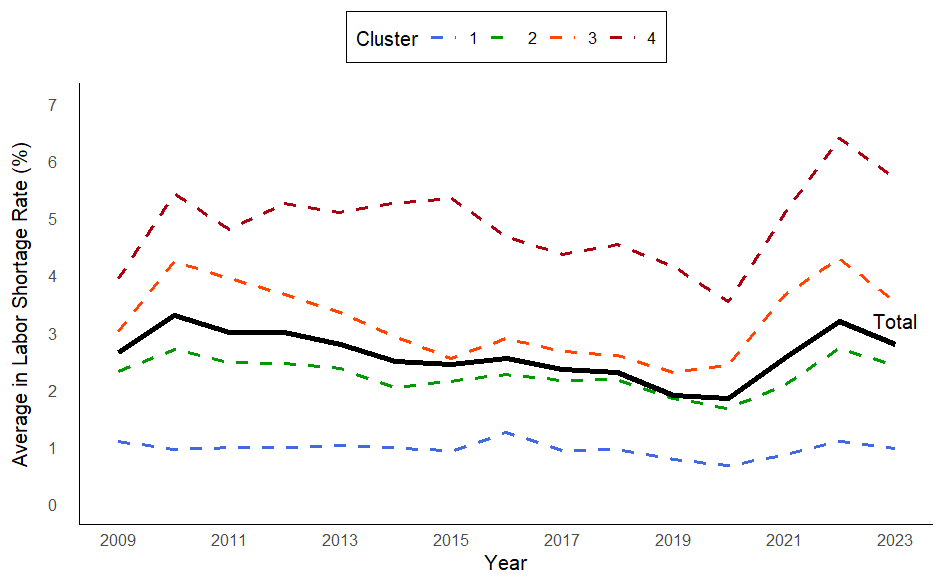
\includegraphics[keepaspectratio]{000066.png}}
\caption{Average Labor Shortage Rate by Cluster
(2009\textasciitilde2023)}
\end{figure}

Figure 6 plots the average labor shortage rate from 2009 to 2023 by
specified clustering in Equation 4.1. The patterns of labor shortage
rate by cluster are quasi-parallel with distinctive fluctuations during
COVID-19. For the 3 years after the pandemic situation, labor shortage
rates increased with heterogeneous slopes: Clusters with higher
intercepts experienced more pronounced increases in workforce
insufficiency. Mainly, Cluster 4 where transportation and storage (490)
and accommodation and food (550) services are included has recorded a
remarkably high labor shortage rate in 2022 during the period. Cluster 3
with the second-highest overall labor shortage rates which followed a
declining pattern between 2010 and 2020 but also experienced more
workforce insufficiency. Considering the composition of Cluster 3 which
includes manufacturing (100) and information and communication (580)
industries, the four main industries with high labor shortage rates also
had stronger impacts on hiring capacity limits. In contrast, Cluster 1,
which comprises energy supply (350), financial and insurance (640), real
estate (680), and education (850) services, exhibited flatter trends
with the lowest labor shortage rate during 15 years. In sum, it is
reasonable to assume that both labor-intensive industries and sectors
which are crucial for skilled workers had more difficulties in hiring
compared to others. Conversely, some industries that have less influence
on economic fluctuations in the labor market context of Korea also have
a lower labor shortage rate with a more stable tendency. The most
distinctive shortage pattern in Cluster 4 is observed, consistently
higher than the 4\% threshold.

\begin{figure}
\centering
\pandocbounded{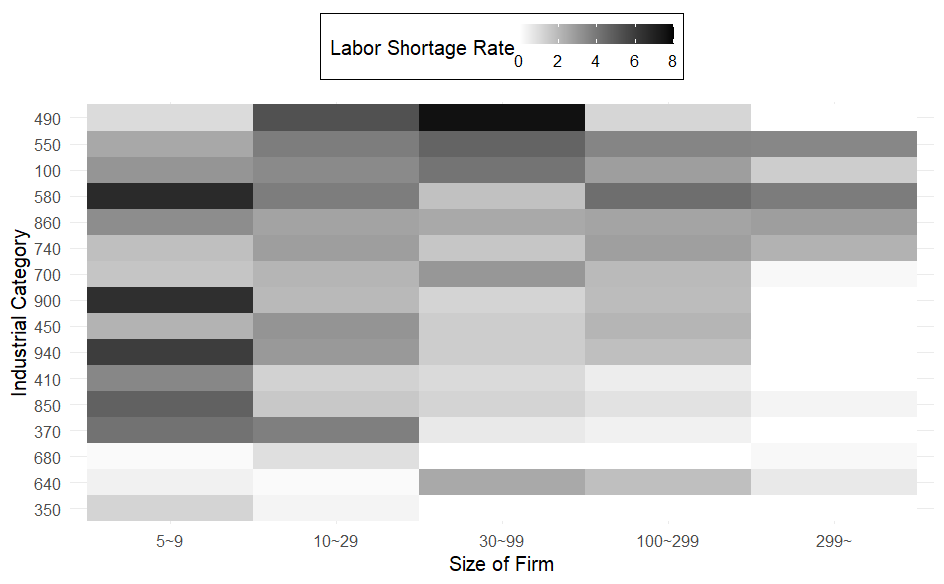
\includegraphics[keepaspectratio]{images/00003e.png}}
\caption{Distribution of Labor Shortage Rates by Firm Size and Industry}
\end{figure}

Figure 7 illustrates how labor shortage status is distributed concerning
the firm size. The order of industrial category implies the descending
order of labor shortage rates by industry on time. As mentioned by Jang
(2018), small and medium-sized enterprises with fewer than 300 employees
generally record higher labor shortage rates, which may suggest SME
avoidance among domestic workers. In-depth, industries in clusters 3 and
4 (except for industry 580) show the highest labor shortage rates in
companies with 30 to 99 employees. Also, services in professional,
scientific, and technical activities (700) and financial and insurance
activities (640) follow a similar pattern. A labor shortage in other
industries is inversely proportional to firm size except the human
health and social work activities (860), which show concentration at
both extremes.

Drawing upon multiple case studies from Nho (2024), the indicator used
in this paper, the labor shortage rate calculated by the number of
vacancies, would not fully represent workforce issues in manufacturing
SMEs. According to the author, aged workers more than 50, immigrants,
and outsourced laborers are widely used nevertheless their skill
deficiency. However, I limit its role as a primal structural cause in
the utilization of overtime work toward existing employees, yet
confirming industrial disparities. However, aligning with the framework
of this paper, the gap in the distribution of labor shortage rates by
size of firms and industries shows which industries of Korea are having
the predominant difficulty in hiring additional adequate workers.

\subsection{Individual Characteristics and Working Hours Distribution
(KLIPS)}\label{individual-characteristics-and-working-hours-distribution-klips}

KLIPS is a nationally representative longitudinal survey conducted by
the Korean Labor Institute (KLI) to track labor market dynamics at the
level of individuals and households in non-rural areas since 1998. KLIPS
introduced sample updates in 2009 and 2018 to expand the sample size and
add more timely and meaningful variables. Using two-stage cluster
systematic sampling based on the Population and Housing Census (PHC),
which is the most standardized benchmark of various social statistics in
Korea, the sample ensures minimal sampling bias relative to the
population. Because the key variables of interest in this study have
been surveyed from the 2009 sample, I selected both the 2009 and 2018
samples. To minimize the external factors related to burnout (e.g.,
health or labor force attachment patterns), only the workers aged over
18, excluding underage individuals, to age 65, the legal first
retirement age, were included in this study (Jacobs \& Piyapromdee,
2016). On that account, the data comprise 52,418 observations from
12,141 individuals in an unbalanced panel format.

Items from the raw KLIPS data were refined into structured variables
with complete definitions in Appendix to facilitate appropriate use in
empirical analysis (see Table A2). First, several characteristics,
widely studied in the labor supply of households, are controlled: Number
of household members, marital status, and monthly income of household.
In formatting the monthly income of the household, sources from labor
activities are excluded.\footnote{Due to mismatch between information in
  household sample and individual sample, I did not deduct wage of
  respondent from entire family income, including labor income of
  others, for accuracy.} Since Simpson et al.~(2024) find gaps between
single and partnered mothers in negative effects on maternal mental
health due to long working hours, marital status in this paper is
qualified by having a spouse. Individual factors related to human
capital resources are respectively controlled: Age, year of education,
year of tenure, and level of job skill. Based on the profile of
occupational criterion categorized by the Korean Standard Classification
of Occupations (KSCO), the level of required skills is ordered regarding
the primal task of a given position (Autor \& Dorn, 2013). Contrary to
working hours, I also include paid vacation offers by employer because
firms might provide paid vacations as partial benefits substituting
compensations. Regarding non-regular worker issues in Korea, the type of
specific contracts, temporary and atypical, is also counted. In a
similar context, the dummy variable identifies public employee control
gaps from working environments in estimations. Nevertheless,
time-invariant variables could not be included in the fixed-effect
estimation, so I adjusted the female dummy in descriptive statistics to
figure out gender disparity in working hour distributions (Shin \& Han,
2016).

Recalling the information related to the dependent variable in previous
chapters for describing its composition, KLIPS provides multiple
sub-indicators of job satisfaction. Instead of using a single overall
job satisfaction, I follow recommendations within computing the average
of relative sub-indicators to induce less bias in estimation: wage,
working hours, value of work, working environment, and quality of
communication (Rose, 2001; Bae, 2008). All components are formed as
5-likert scales, from extremely dissatisfied (1) to extremely satisfied
(5). Through reorganizing as 21 ordinal scales, less information loss
may allow latent variable models under the assumption of continuous
function for more accurate threshold econometric estimations. With the
main objective of this paper, I specified working hours during a week,
as a baseline information of study, into working days per week and
average working hours per day. In counterpoint to previous studies on
working hours, I expect new findings on how the intensity of working
hour allocation in the same period impacts. To exclude outliers,
individuals working more than 21.5 hours per day, the legal limit of
daily work time, are not included (K. Kim, 2024). Considering the
receiving compensation for workers, I simply use overall wage rates,
salary divided by entire worked hours during the same term. Although
Chung et al.~(2018) differentiate between overtime premiums and normal
wages in assessing the negative satisfaction of overtime workers, I
rather choose real wages regardless of various types in calculating wage
compensations.\footnote{KLIPS provides information on paycheck methods,
  types of payroll calculation, level of wages, and incentives. However,
  due to missing data on each criterion, it was impossible to specify
  sources of compensation in this study.} Also, given the ongoing
situation that an inclusive wage system is widely adopted in
considerable firms, a comprehensive measure of compensation is needed to
incorporate the entire sample. Hence, it is sufficiently validated that
I control the effect of earning with a single variable.

\begin{table}[!h]
\centering\centering
\caption{\label{tab:unnamed-chunk-8}Summary Statistics of Demographic Characteristics}
\centering
\resizebox{\ifdim\width>\linewidth\linewidth\else\width\fi}{!}{
\fontsize{11}{13}\selectfont
\begin{threeparttable}
\begin{tabular}[t]{lccc}
\toprule
Variable & Non-Overtime Worker & Overtime Worker & Total\\
\midrule
Age & 42.7 & 43.42 & 42.93\\
 & {}[11.12] & {}[11.22] & {}[11.16]\\
Female Ratio & 0.463 & 0.326 & 0.418\\
 & {}[0.499] & {}[0.469] & {}[0.493]\\
Years of Education & 13.93 & 12.91 & 13.6\\
\addlinespace
 & {}[2.617] & {}[2.678] & {}[2.680]\\
Household Size & 3.244 & 3.164 & 3.218\\
 & {}[1.163] & {}[1.228] & {}[1.185]\\
Marital Status & 0.693 & 0.667 & 0.684\\
 & {}[0.461] & {}[0.471] & {}[0.465]\\
\addlinespace
Household Income & 23.11 & 17.3 & 21.23\\
 & {}[78.25] & {}[62.27] & {}[73.52]\\
\hline\noalign{\vskip -0.1ex}
Observations & 35,507 & 16,911 & 52418\\
\bottomrule
\end{tabular}
\begin{tablenotes}
\item[1] Standard deviations in brakets.
\end{tablenotes}
\end{threeparttable}}
\end{table}

Table 3 shows prominent differences between overtime and non-overtime
worker groups in the female ratio and non-labor income. Consistent with
Shin \& Han (2016), a 13.7\%p gap between groups shows the difficulty of
engaging in overtime work for female workers. Derived from arguments
that overworking norms in organizations discourage the labor force
participation of women, long working-hour practices are seemingly more
frequent in male-dominated work environments. Overtime worker group has
fewer non-labor income sources, confirming approximately 58,000 KRW
monthly gap on average. As a number of studies claim that insufficient
earnings of households lead to longer work, individual impacts from
overwork might be aggravated by income inequality (Park \& Park, 2019;
Lim \& Lee, 2024).

\begin{table}[!h]
\centering\centering
\caption{\label{tab:unnamed-chunk-9}Summary Statistics of Labor Characteristics}
\centering
\resizebox{\ifdim\width>\linewidth\linewidth\else\width\fi}{!}{
\fontsize{11}{13}\selectfont
\begin{threeparttable}
\begin{tabular}[t]{lccc}
\toprule
Variable & Non-Overtime Worker & Overtime Worker & Total\\
\midrule
Dependant Variable &  &  & \\
\hline\noalign{\vskip -0.1ex}\\
Job Satisfaction & 3.432 & 3.23 & 3.367\\
 & {}[0.488] & {}[0.511] & {}[0.504]\\
\hline\noalign{\vskip -0.1ex}
Average Working Time &  &  & \\
\hline\noalign{\vskip -0.1ex}\\
Weekly Working Hours & 37.93 & 51.13 & 42.19\\
\addlinespace
 & {}[6.023] & {}[8.759] & {}[9.347]\\
Daily Working Hours & 7.709 & 8.898 & 8.093\\
 & {}[1.108] & {}[2.146] & {}[1.621]\\
Weekly Working Days & 4.926 & 5.854 & 5.225\\
 & {}[0.514] & {}[0.699] & {}[0.724]\\
\hline\noalign{\vskip -0.1ex}
\addlinespace
Average in Wage &  &  & \\
\hline\noalign{\vskip -0.1ex}\\
Hourly Wage & 16.98 & 11.83 & 15.32\\
 & {}[10.38] & {}[6.853] & {}[9.690]\\
Monthly Wage & 278.2 & 251.8 & 269.7\\
 & {}[168.3] & {}[134.6] & {}[158.7]\\
\hline\noalign{\vskip -0.1ex}
\addlinespace
Working Environment &  &  & \\
\hline\noalign{\vskip -0.1ex}\\
Paid Vacation Provided & 0.688 & 0.507 & 0.629\\
 & {}[0.463] & {}[0.500] & {}[0.483]\\
Public Employee & 0.0624 & 0.0212 & 0.0491\\
 & {}[0.242] & {}[0.144] & {}[0.216]\\
\addlinespace
Temporary Contract & 0.23 & 0.234 & 0.231\\
 & {}[0.421] & {}[0.423] & {}[0.422]\\
Atypical Contract & 0.0922 & 0.1 & 0.0948\\
 & {}[0.289] & {}[0.300] & {}[0.293]\\
Years of Tenure & 8.319 & 7.436 & 8.034\\
\addlinespace
 & {}[7.730] & {}[6.783] & {}[7.449]\\
Labor Shortage Rate & 2.252 & 2.858 & 2.447\\
 & {}[1.866] & {}[2.334] & {}[2.048]\\
\hline\noalign{\vskip -0.1ex}
Observations & 35,507 & 16,911 & 52418\\
\bottomrule
\end{tabular}
\begin{tablenotes}
\item[1] Standard deviations in brakets.
\item[2] Level of job satisfaction is calculated as an average value of 5 domains in job satisfaction. Detailed information is provided in Appendix (see Table A3.
\end{tablenotes}
\end{threeparttable}}
\end{table}

Related to the main interest of the research, Table 4 shows that
overtime workers experience a lower level of job satisfaction, almost
equal to the one scale (0.25 scores), including all components (see
Table A3). With a one-year gap in educational level, as shown in Table
3, a similar gap in professional experiences is observed as well. The
different levels of human capital resources between the two groups
seemingly point out a correlation between long working hours and lower
levels of skilled occupation, further discussed in Table 6. Clearly, a
big difference in working hours between the two groups is shown, 51.13
hours on average for overtime workers compared to 37.93 hours. In that
sense, it is useful to describe how this gap is created from the
composition of the workweek, in more detail as will be argued later in
Table 5.

Parallel to the gap in the non-labor income of households, overtime
workers are less compensated than non-overtime workers with less paid
vacation offers. The average level of wage compensation rates for
overtime workers is almost 30\% less (5,150 KRW in
approximation)---additionally, individuals in overtime group work about
26.31\% less at firms where assist paid time off. In contrast to the
paid salary gap of 9.49\% with 264,000 KRW, rounded at three decimal
places, low wage rates might cause workers to be motivated to
participate in overtime work for a needed amount of income (Park \&
Park, 2019; M. Kim, 2023; Lim \& Lee, 2024). The described information
in the table might show that predominant inequality in income and
compensation between groups is also related to the capacity of
establishment on human resources expenses. It is well known that the
public sector tends to be more sensitive with legal institutions
including working hour limits, the ratio of public employees is
presented at a level of about three times fewer overtime workers.
Possibly, higher labor shortage rates on the market where overtime
worker groups are engaged provide reasonable presumptions on the
mentioned status above. In sum, it is reasonable to assume that serving
overtime work in Korea can be related to secondary labor market
characteristics (Jang, 2018).

\begin{table}[!h]
\centering\centering
\caption{\label{tab:unnamed-chunk-10}Descriptive Statistics of Working Schedules}
\centering
\fontsize{11}{13}\selectfont
\begin{threeparttable}
\begin{tabular}[t]{lccc}
\toprule
Working Days per Week & Non-Overtime Worker & Overtime Worker & Total\\
\midrule
A Single Day & 5.3333 & 0 & 5.3333\\
 & {}[2.8935] & {}[0] & {}[2.8935]\\
 & (0.194\%) & (0\%) & (0.132\%)\\
Two Days & 7.2991 & 0 & 7.2991\\
 & {}[3.0393] & {}[0] & {}[3.0393]\\
\addlinespace
 & (0.918\%) & (0\%) & (0.622\%)\\
Three Days & 7.5536 & 17.2571 & 8.3353\\
 & {}[2.6131] & {}[1.6808] & {}[3.6720]\\
 & (2.25\%) & (0.414\%) & (1.658\%)\\
Four Days & 7.9696 & 15.5645 & 10.7931\\
\addlinespace
 & {}[2.0323] & {}[3.6777] & {}[4.5932]\\
 & (2.732\%) & (3.394\%) & (2.946\%)\\
Five Days & 7.789 & 9.7999 & 7.9813\\
 & {}[0.8404] & {}[1.1168] & {}[1.0524]\\
 & (90.782\%) & (20.153\%) & (67.996\%)\\
\addlinespace
Six Days & 5.6614 & 8.5461 & 8.2929\\
 & {}[1.2667] & {}[1.3470] & {}[1.5692]\\
 & (2.864\%) & (62.498\%) & (22.103\%)\\
Seven Days & 4.3214 & 7.2551 & 7.1418\\
 & {}[1.3020] & {}[1.6022] & {}[1.6889]\\
\addlinespace
 & (0.259\%) & (13.541\%) & (4.544\%)\\
\hline\noalign{\vskip -0.1ex}
Total & 7.7095 & 8.8982 & 8.093\\
 & {}[1.1085] & {}[2.1464] & {}[1.6209]\\
 & (100\%) & (100\%) & (100\%)\\
\bottomrule
\end{tabular}
\begin{tablenotes}
\item[1] Standard deviations in brakets.
\item[2] Percentage by column variable in parentheses
\end{tablenotes}
\end{threeparttable}
\end{table}

Approximately doubled standard deviations in daily working hours for
overtime workers, as Table 5 shows, imply a more irregular schedule in
the overtime worker group. As the current labor institutions suggest,
non-overtime workers are seemingly followed, 90.782\% in general, by a
5-day workweek. A quarter of overtime workers intensively serve more
hours per day on average within a 5-day workweek or less in contrast to
others working for 6 days or even every day during a week. Holiday work
is more frequent in overtime use, and several workers who already serve
full-time additionally demand to be present in their workplace. As I
noted earlier in Equation 4.5a of Estimation Method, two primal patterns
of overtime work need to be assessed in a way as follows: Which
compositions more negatively impact the satisfaction of workers, between
working during the weekend or intensive work of more than 8 hours per
day?

\begin{table}[!h]
\centering\centering
\caption{\label{tab:unnamed-chunk-11}Descriptive Statistics of Working Environment}
\centering
\resizebox{\ifdim\width>\linewidth\linewidth\else\width\fi}{!}{
\fontsize{11}{13}\selectfont
\begin{threeparttable}
\begin{tabular}[t]{lccc}
\toprule
Variable & Non-Overtime Worker & Overtime Worker & Total\\
\midrule
Level of Job Skill &  &  & \\
\hline\noalign{\vskip -0.1ex}\\
- low-skilled & 6494 & 4680 & 11174\\
 & {}[18.29] & {}[27.67] & {}[21.32]\\
- middle-skilled & 17685 & 8913 & 26598\\
 & {}[49.81] & {}[52.71] & {}[50.74]\\
\addlinespace
- high-skilled & 11328 & 3318 & 14646\\
 & {}[31.90] & {}[19.62] & {}[27.94]\\
\hline\noalign{\vskip -0.1ex}
Size of Firm &  &  & \\
\hline\noalign{\vskip -0.1ex}\\
- 5 \textasciitilde{} 9 employees & 6286 & 4481 & 10767\\
 & {}[17.70] & {}[26.50] & {}[20.54]\\
\addlinespace
- 10 \textasciitilde{} 29 employees & 8277 & 4501 & 12778\\
 & {}[23.31] & {}[26.62] & {}[24.38]\\
- 30 \textasciitilde{} 99 employees & 7397 & 3332 & 10729\\
 & {}[20.83] & {}[19.70] & {}[20.47]\\
- 100 \textasciitilde{} 299 employees & 4316 & 1829 & 6145\\
\addlinespace
 & {}[12.16] & {}[10.82] & {}[11.72]\\
- 300 or more employees & 9231 & 2768 & 11999\\
 & {}[26.00] & {}[16.37] & {}[22.89]\\
\hline\noalign{\vskip -0.1ex}
Region of Firm Location &  &  & \\
\hline\noalign{\vskip -0.1ex}\\
- capital area & 18215 & 7718 & 25933\\
\addlinespace
 & {}[51.30] & {}[45.64] & {}[49.47]\\
- metropolitan cities & 9066 & 4731 & 13797\\
 & {}[25.53] & {}[27.98] & {}[26.32]\\
- other provinces & 8226 & 4462 & 12688\\
 & {}[23.17] & {}[26.39] & {}[24.21]\\
\hline\noalign{\vskip -0.1ex}
\addlinespace
Observations & 35507 & 16911 & 52418\\
 & {}[100] & {}[100] & {}[100]\\
\bottomrule
\end{tabular}
\begin{tablenotes}
\item[1] Percentage by column variable in brakets.
\end{tablenotes}
\end{threeparttable}}
\end{table}

Reminding both lower level of education and professional experiences in
overtime workers compared to the another group, Table 6 shows the
composition of overtime workers in the occupation that 9.38\%p more in
low-skilled position and 12.28\%p less in high-skilled demanded position
in general. In other words, the issue of overtime work is more weighted
toward low-skilled occupations, such as services, sales, and manual type
of jobs in general. As Nho (2013) observes, workers allocate office
hours more than the threshold of regular work (40 hours per week) in
small businesses with less than 30 employees. With recollecting that
labor shortage is more frequent in SMEs, as has been noted earlier,
overtime work is seemingly more often in small-sized firms.

\begin{table}[!h]
\centering\centering
\caption{\label{tab:unnamed-chunk-12}Overtime Worker and Working Hour Distribution by Cluster}
\centering
\fontsize{11}{13}\selectfont
\begin{threeparttable}
\begin{tabular}[t]{lccc}
\toprule
List of clusters & Non-Overtime Worker & Overtime Worker & Total\\
\midrule
Cluster 1 & 37.054 & 51.031 & 39.925\\
 & {}[7.571] & {}[10.662] & {}[10.039]\\
 & 6072 & 1570 & 7642\\
Cluster 2 & 37.513 & 50.478 & 41.803\\
 & {}[6.382] & {}[7.998] & {}[9.254]\\
\addlinespace
 & 16213 & 8017 & 24230\\
Cluster 3 & 39.418 & 49.205 & 42.397\\
 & {}[3.112] & {}[6.631] & {}[6.356]\\
 & 10624 & 4649 & 15273\\
Cluster 4 & 36.515 & 56.461 & 46.633\\
\addlinespace
 & {}[7.364] & {}[10.683] & {}[13.567]\\
 & 2598 & 2675 & 5273\\
\hline\noalign{\vskip -0.1ex}\\
Total & 37.932 & 51.126 & 42.188\\
 & {}[6.023] & {}[8.759] & {}[9.347]\\
 & 35507 & 16911 & 52418\\
\bottomrule
\end{tabular}
\begin{tablenotes}
\item[1] Standard deviations in brakets. The number below each cell indicates the frequency (sample size) of the respective subgroup.
\end{tablenotes}
\end{threeparttable}
\end{table}

According to the working hour distribution in Table 7, average working
hours per week for non-overtime workers are concentrated in the upper
30-hour range, while its concentration for overtime workers is around 50
hours with larger standard deviations. Align with the labor shortage
pattern as cluster specification process, significantly long working
hours, about 56.461 hours per week within half of the workers in the
overtime group, are observed in Cluster 4. A remarkable labor shortage
in transportation and storage (490) and accommodation and food (550)
services, more than 4\% overall, is not negligible in the discussion of
overtime work issues. Cluster 3, where the second highest labor shortage
rates are exhibited, has the longest working hours, 39.418 hours, with
the smallest standard deviation in a non-overtime group. Relatively
engaged in high levels of labor regardless of overtime schedule in
general, 42.397 hours per week in total, patterns of Cluster 3 might
imply that the structure of the industry itself inherently demands an
intensive workload. For example, Jee (2021) claims that approximately
38.6\% of workers in the ICT industry are engaged in \emph{crunch mode},
a deadline-driven work compression, for 3.22 months per year on average.
Concurrent with \emph{crunch mode} in ICT, the difficulty in adjusting
labor input on immediate labor demands for certain merchandise
production in the manufacturing industry might cause intensive and
irregular workloads for employees (Nho, 2024). In sum, heterogeneous
patterns in working hour distributions, observed in Cluster 3 and
Cluster 4 which exhibit higher labor shortages than the average, imply
different characteristics of overwork structure. Overwork in Cluster 4
can be conceptualized as polarized working hours with the largest
overtime-worker ratio in on-site service sectors. Work overload in
Cluster 3 intensifies under project deadlines or production
inflexibility in workplaces rather than permanent schedules with longer
working hours due to service management. So, there is a scope to
consider that it is reflected in the difference between labor-intensive
industry and skilled-workforce-demanded industry.

The tendency derived from data shows how the features of overtime
workers were structured in Korea from 2009 to 2023. Both labor shortage
and long working hours are exhibited in labor-intensive industries and
occupations with smaller-sized firms. Relatively low levels of human
capital and compensations for overtime workers were distinctive findings
in Data.\footnote{The general characteristics of overtime workers,
  compared to non-overtime workers, might not capture demanded overwork
  due to needed skill-force which is described as the profiles of
  workers included in Cluster 3. I limit my overall interpretation of
  comparative statistics.} Overtime work in Korea might be considerably
rooted in the dualized labor market problem as a structural cause. Here,
there is a concern that primal differences between the two groups might
create bias in the estimation, as predominant negative working
conditions matter rather than excessive working hours on job
satisfaction. However, negative effects from overtime work are still
observable because this paper aims to study how additional overtime
negatively imposes on the disutility of workers, while controlling other
determinants, within the squared utility function as Rätzel (2012)
suggests.

\newpage

\section{ESTIMATION RESULTS}\label{estimation-results}

The following chapter presents the results corresponding to the two core
research questions outlined in the Estimation Method. Using Ordinary
Least Squares (OLS) with high-dimensional fixed effects, the impact of
labor shortage rates on individual working hours is assessed in the
first stage. The 2,771 singleton observations are automatically omitted,
defined as individuals with only a single appearance. In a subsequent
stage, Equations 4.4 and 4.5 estimate the impact of overtime work on job
satisfaction. Using the ordered logit with fixed effects, estimated
results yield the marginal probability of attaining higher levels of the
ordinal outcome. Equation 4.4a and Equation 4.5a, the auxiliary
equations, investigate how job satisfaction is affected by the density
of the working schedule. Regarding the lacked within-individual
variation problem in outcome indicators, 2,775 observations are excluded
(i.e., all-positive or all-negative responses). Using the Blow-Up and
Cluster (BUC) approach, 658,624 pseudo-observations are employed for
conditional likelihood estimation to replicate the binary response at
each cut point of the latent outcome.

To connect both aforementioned stages, the results of 2SPS-IV are
presented in a subsequent section of this chapter. As the first stage of
baseline estimation drops 2,771 singleton observations, Equation 4.4 and
Equation 4.5 only include predicted working hours for 49,647
observations from Equation 4.1. Subsequently, 657,681
pseudo-observations are used for the IV odds estimation. For 2SPS-IV
conditions, the validity of robust estimation is testified through Table
8, Equation 4.4, and Figure 8. As the F-statistic of first-stage
estimations is plausibly high, the used IV satisfies a high correlation
with the endogenous treatment variable. The results of the exclusion
restriction test are provided in Table 10. Demonstrated results show
that IV does not directly intervene in effects on outcome indicators. As
I described the ACR theorem in the Estimation Method, the share of
compliance is visualized in Figure 8. Using the separated CDF
differences of all clusters, I present that the monotonicity assumption
is respected in 2SPS-IV procedures.

\subsection{Baseline Estimation
Results}\label{baseline-estimation-results}

The following section presents the baseline estimation results in a
two-stage framework. The presenting empirical framework comprises two
core relationships: (1) labor shortage and working hours, and (2)
working hours and job satisfaction. The positive relationship between
labor shortage rates and individual working hours empirically shows that
the market-level variable also imposes individual variation in the
volume of labor. The effects of working hours on individual job
satisfaction exhibit a concave relation, both under- and over-employment
are less preferred than the optimal working hours. As the institutional
reference of full-time work, 40 hours per week, individual preference
for full-time work serves as a significant criterion to determine the
negative response of overtime work on average regarding the argument of
Rätzel (2012). Overall, the above-mentioned correlations among labor
shortage, working hours, and individual satisfaction suppose the
conditions on how employees fail to optimize their labor force
participation.

The first stage of baseline estimation includes three equations that
formulate the relation between labor shortage rates and individual
working hours: Equations 4.1, 4.2, and 4.3. Since Equation 4.1
investigates the linearized association between the intensity of market
constraint and individual working hours, it shows how exogenous labor
shortage shock tends to increase the working hours of employees in
general settings (Hart, 2004; Barnow et al., 2013). As clusters are
structured by the degree of labor shortage fluctuation during 15 years
of observation through hierarchical clustering, Equation 4.2 shows the
between-variance of variance in shortage effects across industries (see
Estimation Method). To show its responsiveness depending on exposure in
each cluster, Equation 4.3 presents how within-variation of labor
shortage rates tends to increase the working hours of individuals
employed in corresponding clusters.

\clearpage
\FloatBarrier
\begin{table}[!h]
\centering\centering
\caption{\label{tab:unnamed-chunk-13}Effects of Industrial Labor Shortage on Working Hour Decisions (Equation 4.1)}
\centering
\resizebox{\ifdim\width>\linewidth\linewidth\else\width\fi}{!}{
\fontsize{11}{13}\selectfont
\begin{threeparttable}
\begin{tabular}[t]{lcccc}
\toprule
Variable & (1) & (2) & (3) & (4)\\
\midrule
Main Explanatory Variable &  &  &  & \\
\hline\noalign{\vskip -0.1ex}\\
Labor Shortage Rates & 0.1204*** & 0.0132** & 0.0051* & 0.0068***\\
 & (0.0292) & (0.0051) & (0.0023) & (0.0015)\\
\hline\noalign{\vskip -0.1ex}
Control Variable &  &  &  & \\
\hline\noalign{\vskip -0.1ex}\\
Hourly Wage & -0.3549*** & -0.0505*** & -0.0146*** & -0.0131***\\
\addlinespace
 & (0.0238) & (0.0033) & (0.0015) & (0.0011)\\
Age & -0.1358*** & 0.0094* & -0.0206*** & -0.0153***\\
 & (0.0221) & (0.0039) & (0.0016) & (0.0011)\\
Years of Education & 1.3160*** & 0.1319*** & 0.0912*** & 0.0392***\\
 & (0.2427) & (0.0369) & (0.0218) & (0.0110)\\
\addlinespace
Household Size & 0.1000 & 0.0156 & 0.0048 & 0.0011\\
 & (0.0810) & (0.0140) & (0.0072) & (0.0047)\\
Marital Status & 0.0968 & 0.0182 & -0.002 & 0.0035\\
 & (0.2409) & (0.0408) & (0.0219) & (0.0132)\\
Household Income & -0.0010* & -0.0001 & -0.0001 & -0.0000\\
\addlinespace
 & (0.0005) & (0.0001) & (0.0000) & (0.0000)\\
Temporary Contract & -0.9254*** & -0.0901*** & -0.0618*** & -0.0219**\\
 & (0.1541) & (0.0271) & (0.0123) & (0.0072)\\
Atypical Contract & -1.9262*** & 0.0250 & -0.2293*** & -0.0441***\\
 & (0.2486) & (0.0442) & (0.0218) & (0.0105)\\
\addlinespace
Paid Vacation Provided & 0.2770* & 0.0608** & 0.0030 & -0.0330***\\
 & (0.1178) & (0.0211) & (0.0098) & (0.0063)\\
Public-Sector Employer & -0.9421*** & -0.1367** & -0.0336 & -0.0634***\\
 & (0.2382) & (0.0485) & (0.0235) & (0.0134)\\
Years of Tenure & 0.1098*** & 0.0143*** & 0.0041** & 0.0032***\\
\addlinespace
 & (0.0189) & (0.0037) & (0.0014) & (0.0009)\\
Constant & 34.3938*** & 6.4602*** & 5.0782*** & 0.6363***\\
 & (3.2843) & (0.4992) & (0.2972) & (0.1509)\\
\hline\noalign{\vskip -0.1ex}
Observations & 49647 & 49647 & 49647 & 49647\\
Number of Individuals & 9370 & 9370 & 9370 & 9370\\
\addlinespace
R-Squared & 0.6637 & 0.6089 & 0.5047 & 0.5479\\
F-statistic & 73.3118*** & 26.2137*** & 74.4904*** & 98.0437***\\
\bottomrule
\end{tabular}
\begin{tablenotes}
\item[1] Robust standard errors clustered at the individual level are reported in parentheses.
\item[2] All models control for industry, job skill level, firm size, and region.
\item[3] Each column corresponds to a different dependent variable: (1) weekly working hours, (2) average daily working hours, (3) working days per week, and (4) binary indicator of overtime participation (Linear Probability Model).
\item[4] F-statistics refer to robust Wald tests clustered at the individual level.
\item[5] Labor shortage rates are measured as percentages ranging from 0 to 100.
\item[6] * p<0.05, ** p<0.01, *** p<0.001
\end{tablenotes}
\end{threeparttable}}
\end{table}
\clearpage

Table 8 shows the results from Equation 4.1, labor shortage rates
generally tend to increase individual working hours. A one percentage
point increase in the labor shortage rates leads to an increase of
approximately 0.12 hours in weekly working hours (column 1) and a 0.68
percentage point increase in the probability of working overtime (column
4), both at the 0.1\% level of statistical significance. While similar
effects are observed for daily working hours on average (column 2) and
number of workdays (column 3), their magnitudes are relatively less
robust: 1\%p increase in labor shortage to 0.0132 hours on average per
day at the 1\% level of statistical significance and more than 0.0051
days per week at the 5\% level of statistical significance. In sum, the
labor shortage rate tends to manifest primarily in the total weekly work
intensification rather than an intervention of the working schedule
allocation.

In contrast to the labor shortage rate, a negative relation with working
hours is exhibited for the compensated higher hourly wage employees.
From the perspective of labor-leisure trade-off, the observed results
align with workers having less motivation to work more (i.e., income
effect). However, paid vacation, often provided as a sort of compensated
leave for overtime work, positively impacts average working hours per
day. Also, summary statistics in Table 4 present that the gap between
overtime and non-overtime worker groups in hourly wage is greater than
the gap in compensated salary per month. While this paper does not
incorporate overtime premiums due to insufficient observations, these
positive associations may reflect institutional compensation mechanisms,
often bundled with intensive working schedules.

The predominant structural characteristics in types of employment
contracts or businesses concurrently influence determining the working
hours of individuals as a potential bias property. Fewer working hours
for employees in public sectors can imply one of the traits related to
standard employment prevalent in Korea (Jang, 2018). On the other hand,
employees with irregular status, such as atypical or temporary
contracts, serve fewer working hours. Moreover, human capital
characteristics also exhibit distinct associations: longer tenure and
higher education are positively correlated with working hours, while
older workers tend to work less. Such statistical patterns show that the
endogenous working hours: individuals also respond to pecuniary
incentives or labor institutions (Hart, 2004; Park \& Park, 2019; Lim \&
Lee, 2024).

\clearpage
\FloatBarrier
\begin{table}[!h]
\centering\centering
\caption{\label{tab:unnamed-chunk-14}Effects of Labor Shortage Cluster Group on Working Hour Decisions (Equation 4.2)}
\centering
\resizebox{\ifdim\width>\linewidth\linewidth\else\width\fi}{!}{
\fontsize{10.5}{12.5}\selectfont
\begin{threeparttable}
\begin{tabular}[t]{lcccc}
\toprule
Variable & (1) & (2) & (3) & (4)\\
\midrule
Main Explanatory Variable &  &  &  & \\
\hline\noalign{\vskip -0.1ex}\\
Labor Shortage Cluster Group (ref. = Cluster 1) &  &  &  & \\
\hline\noalign{\vskip -0.1ex}
- Cluster 2 & 0.5840 & -0.0358 & 0.0816* & 0.0386*\\
 & (0.4943) & (0.1063) & (0.0337) & (0.0193)\\
- Cluster 3 & 0.4185 & -0.0679 & 0.0791* & 0.0086\\
\addlinespace
 & (0.5288) & (0.1063) & (0.0379) & (0.0219)\\
- Cluster 4 & 2.5235*** & 0.2890* & 0.0738 & 0.0729**\\
 & (0.7224) & (0.1413) & (0.0525) & (0.0274)\\
\hline\noalign{\vskip -0.1ex}
Control Variable &  &  &  & \\
\hline\noalign{\vskip -0.1ex}\\
Hourly Wage & -0.3548*** & -0.0505*** & -0.0146*** & -0.0131***\\
\addlinespace
 & (0.0236) & (0.0032) & (0.0015) & (0.0011)\\
Age & -0.1415*** & 0.0096* & -0.0210*** & -0.0156***\\
 & (0.0222) & (0.0039) & (0.0016) & (0.0011)\\
Years of Education & 1.3100*** & 0.1303*** & 0.0918*** & 0.0382***\\
 & (0.2422) & (0.0366) & (0.0218) & (0.0110)\\
\addlinespace
Household Size & 0.1059 & 0.0160 & 0.0052 & 0.0018\\
 & (0.0813) & (0.0141) & (0.0072) & (0.0047)\\
Marital Status & 0.1168 & 0.0232 & -0.0033 & 0.0039\\
 & (0.2414) & (0.0407) & (0.0219) & (0.0133)\\
Household Income & -0.0011* & -0.0001 & -0.0001 & -0.0000\\
\addlinespace
 & (0.0005) & (0.0001) & (0.0000) & (0.0000)\\
Temporary Contract & -0.9639*** & -0.0929*** & -0.0642*** & -0.0229**\\
 & (0.1553) & (0.0275) & (0.0123) & (0.0072)\\
Atypical Contract & -1.9447*** & 0.0378 & -0.2381*** & -0.0473***\\
 & (0.2528) & (0.0446) & (0.0220) & (0.0105)\\
\addlinespace
Paid Vacation Provided & 0.2980* & 0.0682** & 0.0029 & -0.0339***\\
 & (0.1204) & (0.0217) & (0.0100) & (0.0064)\\
Public-Sector Employer & -0.9869*** & -0.1537** & -0.0274 & -0.0625***\\
 & (0.2449) & (0.0503) & (0.0234) & (0.0134)\\
Years of Tenure & 0.1142*** & 0.0139*** & 0.0046** & 0.0035***\\
\addlinespace
 & (0.0191) & (0.0038) & (0.0014) & (0.0009)\\
Constant & 34.3015*** & 6.5066*** & 5.0296*** & 0.6454***\\
 & (3.3046) & (0.5006) & (0.2988) & (0.1516)\\
\hline\noalign{\vskip -0.1ex}
Observations & 49647 & 49647 & 49647 & 49647\\
Number of Individuals & 9370 & 9370 & 9370 & 9370\\
\addlinespace
R-Squared & 0.6621 & 0.6066 & 0.5033 & 0.5469\\
F-statistic & 63.9414*** & 24.3476*** & 65.5877*** & 86.7990***\\
\bottomrule
\end{tabular}
\begin{tablenotes}
\item[1] Robust standard errors clustered at the individual level are reported in parentheses.
\item[2] All models control for industry, job skill level, firm size, and region.
\item[3] Each column corresponds to a different dependent variable: (1) weekly working hours, (2) average daily working hours, (3) working days per week, and (4) binary indicator of overtime participation (Linear Probability Model).
\item[4] F-statistics refer to robust Wald tests clustered at the individual level.
\item[5] * p<0.05, ** p<0.01, *** p<0.001
\end{tablenotes}
\end{threeparttable}}
\end{table}
\clearpage

Compared to Table 8, illustrating quasi-linear shock on individual
working hour determination, the results in Table 9 demonstrate
structural discontinuity of shortage constraints across industrial
clusters. Refers to Cluster 1, the presenting results capture
between-group estimations based on long-term structural disparities
across industry groups. Equation 4.2 excludes industry-level fixed
effects to avoid multi-collinearity since the set of cluster dummies
incorporates industry-level time-series patterns of labor shortages.
Hence, the coefficients in Table 9 include both structural
discontinuities in labor shortage effects and inter-industry
heterogeneity.

Estimated results of Equation 4.2 reflect distinctive effects on cluster
4 at a glance, as suggested by descriptive statistics of overtime
workers and working hour distribution across clusters from Table 7.
Compared to the reference group which reports the lowest overall labor
shortage rates, employees in transportation, storage, accommodation, and
food service activities (Cluster 4) work 2.5235 hours per week more at a
0.1\% level of statistical significance. Moreover, workers in Cluster 4
are likely to participate more in overtime work at 7.29\%p with a 0.1\%
level of statistical significance. Despite a relatively weak level of
statistical significance of 5\%, it is possible to clarify that more
than 0.2890 hours per day are particularly imposed to work more for
individuals in Cluster 4, compared to the other industries.

In sum, Equation 4.2 reveals a structural break with concentrated
positive effects on Cluster 4 compared to the smooth trend of labor
shortage effect on individual working hours, suggested in Equation 4.1.
The overall linear slope in Equation 4.1 is disproportionately driven by
Cluster 4, a crucial source of variation in constructing the
between-cluster heterogeneity. However, the average effects of labor
shortage, suggested in Equations 4.1 and 4.2, do not sufficiently
integrate responses on working hour variations relative to the shift in
individual conditions across the time. Hence, I identify the
within-cluster elasticity of labor shortage on working hours to
interpret labor shortage as a driver of involuntary overwork through
Equation 4.3.

\clearpage
\FloatBarrier
\begin{table}[!h]
\centering\centering
\caption{\label{tab:unnamed-chunk-15}Effects of Labor Shortage Cluster Group on Working Hour Decisions (Equation 4.3)}
\centering
\resizebox{\ifdim\width>\linewidth\linewidth\else\width\fi}{!}{
\fontsize{11}{13}\selectfont
\begin{threeparttable}
\begin{tabular}[t]{lcccc}
\toprule
Variable & (1) & (2) & (3) & (4)\\
\midrule
Main Explanatory Variable &  &  &  & \\
\hline\noalign{\vskip -0.1ex}\\
Cluster X Labor Shortage Rates &  &  &  & \\
\hline\noalign{\vskip -0.1ex}\\
- Cluster 1 X Labor Shortage Rates & 0.0153 & 0.0080 & -0.0018 & 0.0019\\
 & (0.0862) & (0.0168) & (0.0069) & (0.0038)\\
- Cluster 2 X Labor Shortage Rates & 0.1841*** & 0.0174* & 0.0104** & 0.0091***\\
\addlinespace
 & (0.0471) & (0.0087) & (0.0039) & (0.0024)\\
- Cluster 3 X Labor Shortage Rates & 0.1407** & 0.0093 & 0.0099* & 0.0082**\\
 & (0.0478) & (0.0077) & (0.0039) & (0.0026)\\
- Cluster 4 X Labor Shortage Rates & 0.1471* & 0.0177 & 0.0023 & 0.0055*\\
 & (0.0585) & (0.0101) & (0.0042) & (0.0024)\\
\hline\noalign{\vskip -0.1ex}
\addlinespace
Control Variable &  &  &  & \\
\hline\noalign{\vskip -0.1ex}\\
Hourly Wage & -0.3566*** & -0.0507*** & -0.0147*** & -0.0131***\\
 & (0.0238) & (0.0032) & (0.0015) & (0.0011)\\
Age & -0.1370*** & 0.0099* & -0.0206*** & -0.0152***\\
 & (0.0224) & (0.0039) & (0.0016) & (0.0011)\\
\addlinespace
Years of Education & 1.2696*** & 0.1239*** & 0.0912*** & 0.0370***\\
 & (0.2373) & (0.0359) & (0.0218) & (0.0109)\\
Household Size & 0.1100 & 0.0169 & 0.0051 & 0.0020\\
 & (0.0815) & (0.0141) & (0.0072) & (0.0047)\\
Marital Status & 0.1148 & 0.0233 & -0.0036 & 0.0034\\
\addlinespace
 & (0.2417) & (0.0408) & (0.0219) & (0.0133)\\
Household Income & -0.0011* & -0.0001 & -0.0001 & -0.0000\\
 & (0.0005) & (0.0001) & (0.0000) & (0.0000)\\
Temporary Contract & -0.9653*** & -0.0917*** & -0.0649*** & -0.0226**\\
 & (0.1559) & (0.0277) & (0.0124) & (0.0072)\\
\addlinespace
Atypical Contract & -1.9555*** & 0.0375 & -0.2387*** & -0.0462***\\
 & (0.2527) & (0.0449) & (0.0219) & (0.0105)\\
Paid Vacation Provided & 0.2796* & 0.0634** & 0.0038 & -0.0344***\\
 & (0.1210) & (0.0217) & (0.0101) & (0.0063)\\
Public-Sector Employer & -0.9816*** & -0.1511** & -0.0283 & -0.0615***\\
\addlinespace
 & (0.2451) & (0.0500) & (0.0234) & (0.0134)\\
Years of Tenure & 0.1135*** & 0.0140*** & 0.0045** & 0.0033***\\
 & (0.0191) & (0.0038) & (0.0014) & (0.0009)\\
Constant & 34.9644*** & 6.5424*** & 5.0719*** & 0.6568***\\
 & (3.2218) & (0.4858) & (0.2975) & (0.1499)\\
\hline\noalign{\vskip -0.1ex}
\addlinespace
Observations & 49647 & 49647 & 49647 & 49647\\
Number of Individuals & 9370 & 9370 & 9370 & 9370\\
R-Squared & 0.6619 & 0.6062 & 0.5033 & 0.5470\\
F-statistic & 59.2962*** & 22.0276*** & 61.4647*** & 80.4280***\\
\bottomrule
\end{tabular}
\begin{tablenotes}
\item[1] Robust standard errors clustered at the individual level are reported in parentheses.
\item[2] All models control for industry, job skill level, firm size, and region.
\item[3] Each column corresponds to a different dependent variable: (1) weekly working hours, (2) average daily working hours, (3) working days per week, and (4) binary indicator of overtime participation (Linear Probability Model).
\item[4] F-statistics refer to robust Wald tests clustered at the individual level.
\item[5] * p<0.05, ** p<0.01, *** p<0.001
\end{tablenotes}
\end{threeparttable}}
\end{table}
\clearpage

Equation 4.3 separates the marginal effects of the labor shortage rate
on working hours based on the interaction between four ordered
industrial clusters and their fluctuation. Estimated results from
Equations 4.1 and 4.2 follow average trends that labor shortage rates
increase the working hours of employed individuals. However, Equation
4.3 presents that its sensitivity is inversely responsive to the average
labor shortage rates holding the same positive relations. Except for
Cluster 1, the size of the coefficient and statistical significance are
almost more distinctive at Cluster 2 and less distinctive at Cluster 4.
Column 1 in Table 10 presents that a 1\%p change in labor shortage rate
increases weekly working hours as 0.1841 hours in Cluster 2, 0.1407
hours in Cluster 3, and 0.1471 hours in Cluster 4. For the linear
probability of overtime participation in column 4, a 1\%p change in
labor shortage rate increases 0.91\%p for Cluster 2, 0.82\%p for Cluster
3, and 0.55\%p for Cluster 4. Especially in Cluster 2, labor shortage
rates also increase by 0.0174 hours of work per day and 0.0104 days per
week at a 5\% level of statistical significance. Cluster 1 which
includes energy supply (350), financial and insurance (640), real estate
(680), and education (850) services does not provide any statistically
significant and robust results for individual working hours responsive
to labor shortage variation.

Holding other working and individual characteristics constant, I confirm
that industry differences, which refer to the labor shortage, alone lead
to longer and more intensive working hour participation within a given
workweek. Furthermore, the shift of model specification in the first
stage does not crucially result in incidental distortion of control
variables estimates. The consistency of effects in control vectors was
observed through their coefficients, standard errors, and level of
statistical significance in Table 8, Table 9, and Table 10.

Based on the results in Table 10, it is reasonable to assume that the
exogenous shock, labor shortage, in individual working hour decisions
exist besides internal determinants. Despite the statistical
insignificance of results in Cluster 1, quasi-monotone responsiveness is
weakly present. High F-statistics in the results of column 1 and column
4, 59.2962 and 80.4280 on each, support valid instrument conditions for
IV estimation. Hence, by assuming Cluster 1 as a reference group, the
predicted working hours of columns 1 and 4 from Equation 4.3 substitute
observed working hours in 2SPS-IV estimation from Equation 4.7 to
Equation 4.8. Relative to the heterogenous responses of labor shortage
presence in each cluster, I visualize the distribution of causal
responses within strata of clustered IV in further stage (see Figure 8).

Using Equations 4.1, 4.2, and 4.3, estimated results of the first stage
confirm that labor shortage rates consistently lead to longer individual
working hours. However, the impact of observed working hours on
individual satisfaction has a crucial limitation regarding its
endogeneity. The pattern of control vectors suggests that the decision
to work overtime may be influenced not only by external market
constraints but also by internal motivation to seek incentives or
benefits from institutions. Since this study aims to clarify that
overtime work causes burnout under pressure, it is imperative to
identify the pure negative effects of over-employment imposed by
exposure to workforce shortage intensity.

Still, the initial association between individual working hours and job
satisfaction in the second stage raises the question of how preferences
of individuals are structured under the distribution of working hours
controlling wages. Under the aforementioned bias, the second stage
approximately reveals a conditional optimal bundle of working hours
given covariates. The second stage presents that excessive and
intensified working schedules decrease the level of individual job
satisfaction. First, I investigate the concave relationship between
working hours and personal satisfaction and whether controlling wage
rates through Equation 4.4 (see Rätzel, 2012). Focusing on the point of
margin, the overtime threshold and its intensity are additionally
assessed through Equation 4.5. Regarding the assumption that
work-related fatigue is driven by the lack of recovery time, this paper
additionally incorporates the density of hours worked per week (Jacobs
\& Piyapromdee, 2016; Pencavel 2016b; Donsimoni, 2020). Through the
decomposition of weekly working hours by the days worked per week,
Equation 4.4a provides how allocated patterns of work exhibit
diminishing utility of workers. Focusing on overtime workers, Equation
4.5a investigates which is the more crucial sub-factor of the working
schedule leading to dissatisfaction: Fewer days without work or
intensive working hours on a given day? The following models, from
Equation 4.4 to Equation 4.5a, employ fixed-effects ordered logit
estimation, and the reported coefficients represent the log Conditional
Odds Ratio (COR) of being at or above a certain level of job
satisfaction.

\clearpage
\FloatBarrier
\begin{table}[!h]
\centering\centering
\caption{\label{tab:unnamed-chunk-16}Relationship between Weekly Working Hours and Job Satisfaction (Equation 4.4 and 4.5)}
\centering
\resizebox{\ifdim\width>\linewidth\linewidth\else\width\fi}{!}{
\fontsize{11}{13}\selectfont
\begin{threeparttable}
\begin{tabular}[t]{lcccc}
\toprule
Variable & (1) & (2) & (3) & (4)\\
\midrule
Main Explanatory Variable &  &  &  & \\
\hline\noalign{\vskip -0.1ex}\\
Overtime Worker X Weekly Working Hours &  &  & -0.0027** & -0.0019*\\
 &  &  & (0.0009) & (0.0009)\\
Weekly Working Hours & -0.0068*** & 0.0522*** & -0.0012 & 0.0546***\\
 & (0.0020) & (0.0081) & (0.0027) & (0.0080)\\
\addlinespace
Weekly Working Hours (Squared) &  & -0.0006*** &  & -0.0006***\\
 &  & (0.0001) &  & (0.0001)\\
\hline\noalign{\vskip -0.1ex}
Control Variable &  &  &  & \\
\hline\noalign{\vskip -0.1ex}\\
Hourly Wage & 0.0489*** & 0.0513*** & 0.0485*** & 0.0510***\\
 & (0.0046) & (0.0044) & (0.0046) & (0.0043)\\
\addlinespace
Age & 0.0062 & 0.0042 & 0.0049 & 0.0034\\
 & (0.0055) & (0.0054) & (0.0054) & (0.0054)\\
Years of Education & -0.1000 & -0.1114 & -0.1012 & -0.1118\\
 & (0.0575) & (0.0578) & (0.0575) & (0.0579)\\
Household Size & -0.0679** & -0.0686** & -0.0682** & -0.0689**\\
\addlinespace
 & (0.0243) & (0.0243) & (0.0243) & (0.0243)\\
Marital Status & 0.1349 & 0.1419* & 0.1356 & 0.1422*\\
 & (0.0703) & (0.0700) & (0.0703) & (0.0700)\\
Household Income & 0.0002 & 0.0002 & 0.0002 & 0.0002\\
 & (0.0002) & (0.0002) & (0.0002) & (0.0002)\\
\addlinespace
Temporary Contract & -0.1458*** & -0.1340*** & -0.1443*** & -0.1331***\\
 & (0.0388) & (0.0388) & (0.0389) & (0.0388)\\
Atypical Contract & -0.3117*** & -0.2866*** & -0.3076*** & -0.2841***\\
 & (0.0547) & (0.0546) & (0.0547) & (0.0546)\\
Paid Vacation Provided & 0.2979*** & 0.2773*** & 0.2914*** & 0.2732***\\
\addlinespace
 & (0.0334) & (0.0334) & (0.0335) & (0.0335)\\
Public-Sector Employer & 0.3114*** & 0.3145*** & 0.3080*** & 0.3120***\\
 & (0.0788) & (0.0788) & (0.0789) & (0.0789)\\
Years of Tenure & -0.0076 & -0.0091 & -0.0077 & -0.0091\\
 & (0.0047) & (0.0047) & (0.0047) & (0.0047)\\
\hline\noalign{\vskip -0.1ex}
\addlinespace
Pseudo-Observations & 658624 & 658624 & 658624 & 658624\\
Observations & 49643 & 49643 & 49643 & 49643\\
Number of Individuals & 9368 & 9368 & 9368 & 9368\\
Pseudo R-Squared & 0.6249 & 0.6259 & 0.625 & 0.6259\\
Log conditional Likelihood & -104200.4 & -103934.88 & -104170.67 & -103920.11\\
\bottomrule
\end{tabular}
\begin{tablenotes}
\item[1] All coefficients are expressed in log-odds. Standard errors clustered at the individual level are reported in parentheses.
\item[2] Expanded through BUC-OLOGIT estimation (Baetschmann et al., 2020).
\item[3] Observations with multiple positive outcomes within groups are excluded due to identification constraints.
\item[4] All models control for industry, occupational category, firm region, and firm size.
\item[5] * p<0.05, ** p<0.01,  *** p<0.001
\end{tablenotes}
\end{threeparttable}}
\end{table}
\clearpage

Table 11 shows the results from Equation 4.4. and 4.5 exhibiting concave
relations between weekly working hours and job satisfaction. The
inverse-U-shaped relationship between working hours and job satisfaction
which I hypothetically assumed confirms a domain in negative utility
from both under- and over-employment of individuals (see Figure 4; see
also Winkelmann \& Winkelmann, 1998; Rätzel, 2012). At a glance, if an
additional hour of work is imposed on individuals, the odds of reporting
higher job satisfaction decrease by approximately 0.68\% per additional
hour worked, holding other factors constant, as suggested in column 1.
However, workers show a higher probability of reaching greater
satisfaction levels up to a certain point, approximately around early 40
hours,\footnote{From Equation 4.4, total working hours per week which
  maximize the probability of accessing the highest level of job
  satisfaction can be derived through solving the first-order condition
  from concave function \(\phi(H_{it})\). Partial derivative of
  \(H_{it}\) on the latent variable \(y^*_{it}\) can be translated as
  \(\frac{\partial \phi}{\partial H_{it}}\) holding other variables
  constant. Therefore
  \(H^*_{it} = - \frac{\beta_1}{2\beta_2} \approx 43.5\).} as indicated
by the positive coefficient on the linear term and the negative
coefficient on the squared term of working hours in column 2. Negative
effects per hour of work are more significant for the group of
individuals who worked more than 40 hours per week at a 1\% level of
statistical significance as results from column 3. Incorporating the
squared term function of working hours, column 4 presents that
additional disutility at a margin of overtime is exhibited as about
0.19\% with relatively small significance (5\%).

Existing literature has long suggested that economic rewards can
positively affect both labor supply and pecuniary utility (Hart, 2004;
C.Green \& Heywood, 2008; Rätzel, 2012; Park \& Park, 2019; M. Kim,
2023; Lim \& Lee, 2024). For this reason, it seems plausible that
additional negative effects on overtime workers from working hours
alongside the squared function of working hours are reported with a
smaller magnitude on both coefficients and statistical significance.
From the results from the given estimation, this paper also
provisionally considers that paid vacation and wages offered by
employers seemingly moderate negative effects from overtime work. For
instance, offering 1,000 KRW more per hour worked gives employees almost
5.2\% more of a higher level of job satisfaction, at 0.1\% statistical
significance. Also, workers who benefited from paid vacation can have a
relatively 31.4\% higher probability of achieving a greater level of
satisfaction compared to others. Still, it remains valid to assume that
excessive working hours reduce non-pecuniary utility, even when monetary
compensation exists. Owing to a number of literature, it is appropriate
to understand that such rewards moderate rather than eliminate the
entire disutility from overwork (Hart, 2004; C.Green \& Heywood, 2008;
Rätzel, 2012; Donsimoni, 2020).

Moreover, while each additional household member is associated with
lower job satisfaction, negative probability of 6.62\% rounded at three
decimal places from the results in column 2, married workers (i.e.,
having a spouse) report a relatively 15.16\% more probability of
increase in satisfaction. To synthesize the aforementioned, negative
impact on individual well-being from additional allocated burden in
parenting or financial support for households that might be considered
as Simpson et al.~(2024) partially argue. Regarding the negative
probability of workers engaged in irregular contracts (e.g., temporary
contracts and atypical types of work), the claim of Russo (2012) is
reaffirmed in this paper as unstable labor conditions negatively impact
occupational satisfaction. In contrast, the public employee can
distinctively have a higher level of job satisfaction, almost 36.96\%
more, as widely recognized as a secured occupation in Korea. Thus,
besides working hours, it is reasonable to assume that high compensation
with standardized working conditions might enhance the profile of decent
jobs although the burden of living from household characteristics
negatively impacts.

Results from the dual structure in Equation 4.4a, decomposing Equation
4.4, do not simply underscore how many working hours are, but how the
distribution of excessive working hours matters for understanding
burnout from individual disutility. Since Table 10 contains a brief
sketch that total working hours per week might exhibit a bell-shaped
function on individual utility, the impact on job satisfaction is
derived as two primal components of allocated structure for the density
of hours worked on a given period through Equation 4.4a. As a result,
Table A4 confirms concave relations from working days per week and
negative linear with average working hours per day as column 3 and
column 4 report while all detailed coefficients of control variables had
similar results as Table 11. Based on column 3, the optimized working
days in maximizing the probability toward the highest level of overall
job satisfaction are 5 days per week in approximation.\footnote{Analogous
  to the approach used to derive the optimal total working hours per
  week, the optimal number of working days \(d^*_{it}\) is calculated by
  solving the first-order condition
  \(\frac{\partial \phi}{\partial d_{it}}=0\). Therefore,
  \(d^*_{it} = - \frac{\beta_2}{2\beta_4} \approx 5.2\) as if other
  variables constantly hold, based on Equation 4.2a.} In contrast to the
concave relationship observed with working days per week, average
working hours per day show a negative quasi-linear, decreasing by 4.7\%
in odds of reaching a higher job satisfaction per additional hour worked
during a day on average. Beyond a single-dimensional view of labor
input, the results show asymmetric effects on subjective utility
regarding the composition of the work schedule.

As Equation 4.5a extends the decomposed model in Equation 4.4a by
conditioning the effects of time allocation on overtime status, Table A5
shows how working hours intensify negative satisfaction on overtime
workers, defined as those who work more than 40 hours per week. The
model includes interaction terms to test if working hours for overtime
workers proportionally aggravate discontentment on its overall
bell-shaped relationship. Adjusted interaction terms are multiplying the
threshold dummy on average hours worked per day and the number of worked
days during a week. In sum, the conditional effect shows that
satisfaction with work more sensitively varies on the time allocation of
workers who already serve more than 40 hours per week. As reported
results of control variables in Table A5 show a close similarity with
Table 11, also the same for Table A4 confirming no differences in its
pattern.

Interestingly, the disutility associated with longer daily working hours
is observed only among overtime workers, with a 7.64\% decrease in the
odds of reporting higher job satisfaction, and no statistically
significant effect for the overall estimation. In contrast, maintaining
the concave relationship found in previous results, each additional
working day per week for overtime workers increases the odds of
reporting higher satisfaction, by approximately 12.19\%. As Pencavel
(2016b) argues, ensuring an appropriate time for recovery with more
consistency might influence not only the performance of workers but also
their exhaustion. Compared to the aforementioned claims, presenting
estimation results had more detailed implications based on the piece of
empirical evidence in Korea: frequent recovery time on each workday is
more focused than the author suggested.

Two key findings from Table A5 impart on how the structure of working
time allocation affects individual welfare. Consistent with prior
literature on burnout, this study finds that intensive working hours per
day for workers who are already engaged in relatively excessive
workloads cause primal satisfaction loss (Maslach \& Leiter, 2016).
Since a larger negative magnitude of coefficient on daily working hours
on average is only observed on overtime workers with statistical
significance, Table A5 shows that additional working hours per day
mainly affect dissatisfaction within the context of fatigue. As more
days of work per week reduce the average unit of requisite work on a
single day, the results can underscore that the concentrated working
hours during a given workday might impact more on individual
dissatisfaction rather than how simply they work more.

To clarify the magnitude of this effect, the marginal rate of
substitution (MRS), interpreted here as a subjective exchange ratio
between daily time intensity and weekly work dispersion, is calculated
based on the estimated coefficients under the constraint of fixed total
working hours. From MRS which is conditional to overtime workers, the
size of negative utility gained from an additional hour on every workday
would be balanced approximately 1.4465 days.\footnote{The rate at which
  average hours worked per day is substituted by working days during a
  week is calculated as follow:
  \(\text{MRS}_{{\bar{h} \rightarrow d} \mid H_{it} > 40} = \frac{MU_{\bar{h}}}{MU_d} = - \frac{\Delta d_{it}}{\Delta \bar{h}_{it}} = -\frac{0.1150}{-0.0795} \approx 1.4465\)}
Provided that a week is combined with 7 days, the feasibility of using
additional workdays to offset daily fatigue may provide only a partial
coping strategy.

Before IV correction, the second stage of baseline estimation shows the
pattern of association between individual working hours and job
satisfaction in the observational setting. Equation 4.4 shows
inverse-U-shaped individual preferences on working hours as a net of
covariate effects. Subsequently, Equation 4.5 provides that the
additional weight on job dissatisfaction for overtime worker is
proportional to their working hours. Auxiliary equations, Equations 4.4a
and 4.5a, support that intensified working hours, namely, a more
concentrated schedule on a single day, are the most crucial factor in
individual job satisfaction. Especially for employees working more than
40 hours, additional longer and intensified working hours on a given
schedule aggravate the non-pecuniary utility loss. A conditional optimal
bundle of working hours, derived by FOC constrained by the control
vector from the utility maximization process, is approximately assumed
at 43.5 hours per week with 5 days on a given workweek. Still, the
possibility of selection bias necessitates an IV-based strategy to
isolate the causal effect of involuntary overtime. Hence, the results
from Equations 4.4 to 4.5a only serve to sketch the primal association
of how employed individuals valued their hours of actual work during
during the sample period (2009 \textasciitilde{} 2022).

The baseline estimations (Equations 4.1 to 4.5a) have illustrated the
causal pathway from labor shortage to burnout. The first stage
(Equations 4.1 to 4.3) confirms that exogenous constraints, defined as
labor shortage rates across industries, regions, and establishment
sizes, significantly increase individual working hours. Labor shortage
rates impact total working hours per week and the decision to overwork
rather than the sub-components of the working schedule. While the total
volume of labor, measured by weekly working hours, is strongly affected
by labor shortage rates, the allocation of hours across days appears
less responsive to such constraints. By the second stage of baseline
estimation, I assume that the negative perception of excessive working
hours is concentrated on overtime workers. This effect is particularly
pronounced among overtime workers, who appear more sensitive to a daily
intensification of work schedules. To clarify the causal effects in the
suggested path, I present how exogenous variations in working hours
caused by labor shortages affect burnout in a subsequent IV-2SPS
estimation.

\subsection{IV Estimation Results}\label{iv-estimation-results}

Baseline estimation with fixed effects at individual and
establish-related identifier levels has a limitation in clarifying the
causal effect of excessive working hours in negative individual
perception. Hence, in this section, I aim to identify how excessive
working hours affect the utility loss of employed individuals using
exogenous variation of working hours within instrument strata, avoiding
reverse causality and incentive-related endogeneity. IV estimation using
2SPS with a non-linear model interpreted as POR serves to connect the
findings from both stages of analysis, eliminating confounders related
to the endogenous property of working hours by labor shortage rates of
each cluster (see Burgess, 2013; Basu et al., 2018). IV-2SPS estimations
substitute observed working hours with predicted working hours from
Equation 4.3, presented in Table 10. Since attributed working hour
variation on each cluster is continuous, it is reasonable to assume,
following the ACR theorem, that individuals are treated by intensity
dispersed in working hour distribution (Angrist \& Imbens, 1995).

Using IV-2SPS estimation necessitates assuming the following conditions
for causal inference: Relevance, exclusion restriction, and
monotonicity. Since this paper assumes that individual working hours are
externally affected by their responsiveness to the labor shortage in
each industrial cluster, high F-statistic reports from the first stage
satisfy valid relevance conditions (see Table 10). For the robustness of
estimation, Equation 4.6 provides a preliminary test for the exclusion
restriction by examining whether the labor shortage rates, clustered by
industry, directly affect subjective satisfaction. Assuming the
monotonically increasing function of IV on working hours that ordered
sets of its strata specify upper and lower bounds, Figure 8 demonstrates
causal responses by approximately comparing CDF between the lowest and
the highest quantile of labor shortage on each cluster (see Manski \&
Pepper, 2000). Concerning such assumptions, Equation 4.7 investigates
the causal effects of working hour treatment on individual job
satisfaction. To isolate its marginal effect on overtime workers,
Equation 4.8 introduces an interaction term that indicates the
interaction between overtime cut-off, institutional reference as 40
hours per week, and instrumented working hours.

The estimation results from Equation 4.6, reported in Table 12, indicate
that labor shortage rates within each industrial cluster do not exert a
direct effect on individual job satisfaction. Rather, their influence
appears to operate indirectly through working hours. Across
specifications with sequentially added control variables (columns 2 to
5), the coefficients for labor shortage rates become statistically
insignificant, reinforcing the validity of the exclusion restriction.

Although the result in column 1 suggests a potential direct effect of
labor shortage rates in Cluster 2, this likely reflects omitted variable
bias (OVB): The effect disappears as multi-level fixed effects and
job-related covariates are incorporated. The estimated results of
control vector are consistent with the pattern observed in Table 11 and
auxiliary Tables A4 and A5. Overall, the findings support the assumption
that labor shortage rates affect burnout only via their influence on
working hours, not through a separate channel.

\FloatBarrier
\begin{table}[!h]
\centering\centering
\caption{\label{tab:unnamed-chunk-17}Preliminary Test on Exclusion Restriction (Equation 4.6)}
\centering
\resizebox{\ifdim\width>\linewidth\linewidth\else\width\fi}{!}{
\fontsize{11}{13}\selectfont
\begin{threeparttable}
\begin{tabular}[t]{lccccc}
\toprule
Variable & (1) & (2) & (3) & (4) & (5)\\
\midrule
Main Explanatory Variable &  &  &  &  & \\
\hline\noalign{\vskip -0.1ex}\\
Cluster X Labor Shortage Rates &  &  &  &  & \\
\hline\noalign{\vskip -0.1ex}\\
- Cluster 1 X Labor Shortage Rates & 0.0104 & 0.0147 & 0.0113 & 0.0140 & 0.0150\\
 & (0.0259) & (0.0269) & (0.0269) & (0.0271) & (0.0272)\\
- Cluster 2 X Labor Shortage Rates & -0.0366** & -0.0221 & -0.0235 & -0.0161 & -0.0161\\
\addlinespace
 & (0.0128) & (0.0127) & (0.0127) & (0.0130) & (0.0130)\\
- Cluster 3 X Labor Shortage Rates & -0.0157 & -0.0064 & -0.0059 & 0.0017 & 0.0022\\
 & (0.0132) & (0.0128) & (0.0128) & (0.0133) & (0.0133)\\
- Cluster 4 X Labor Shortage Rates & -0.0224 & -0.0196 & -0.0170 & -0.0147 & -0.0149\\
 & (0.0120) & (0.0115) & (0.0116) & (0.0116) & (0.0117)\\
\hline\noalign{\vskip -0.1ex}
\addlinespace
Control Variable &  &  &  &  & \\
\hline\noalign{\vskip -0.1ex}\\
Hourly Wage &  & 0.0525*** & 0.0522*** & 0.0517*** & 0.0520***\\
 &  & (0.0045) & (0.0045) & (0.0045) & (0.0045)\\
Age &  & 0.0052 & 0.0053 & 0.0064 & 0.0056\\
 &  & (0.0054) & (0.0054) & (0.0055) & (0.0055)\\
\addlinespace
Years of Education &  & -0.0888 & -0.0965 & -0.0960 & -0.0965\\
 &  & (0.0572) & (0.0570) & (0.0572) & (0.0574)\\
Household Size &  & -0.0701** & -0.0688** & -0.0678** & -0.0710**\\
 &  & (0.0242) & (0.0243) & (0.0243) & (0.0243)\\
Marital Status &  & 0.1219 & 0.1261 & 0.1260 & 0.1289\\
\addlinespace
 &  & (0.0705) & (0.0704) & (0.0703) & (0.0701)\\
Household Income &  & 0.0002 & 0.0002 & 0.0002 & 0.0002\\
 &  & (0.0002) & (0.0002) & (0.0002) & (0.0002)\\
Temporary Contract &  & -0.1344*** & -0.1338*** & -0.1347*** & -0.1361***\\
 &  & (0.0386) & (0.0386) & (0.0386) & (0.0387)\\
\addlinespace
Atypical Contract &  & -0.3123*** & -0.3076*** & -0.3092*** & -0.3099***\\
 &  & (0.0544) & (0.0543) & (0.0544) & (0.0543)\\
Paid Vacation Provided &  & 0.3179*** & 0.3162*** & 0.3046*** & 0.3021***\\
 &  & (0.0332) & (0.0332) & (0.0333) & (0.0333)\\
Public-Sector Employer &  & 0.3392*** & 0.3390*** & 0.3304*** & 0.3277***\\
\addlinespace
 &  & (0.0779) & (0.0778) & (0.0780) & (0.0784)\\
Years of Tenure &  & -0.0070 & -0.0070 & -0.0076 & -0.0077\\
 &  & (0.0047) & (0.0047) & (0.0047) & (0.0047)\\
\hline\noalign{\vskip -0.1ex}
Job-Level Control & No & No & Yes & Yes & Yes\\
Size of Firm Control & No & No & No & Yes & Yes\\
\addlinespace
Region-Level Control & No & No & No & No & Yes\\
\hline\noalign{\vskip -0.1ex}\\
Pseudo-Observations & 658624 & 658624 & 658624 & 658624 & 658624\\
Observations & 49643 & 49643 & 49643 & 49643 & 49643\\
Number of Individuals & 9368 & 9368 & 9368 & 9368 & 9368\\
Pseudo R-Squared & 0.6141 & 0.6236 & 0.6237 & 0.6239 & 0.6242\\
\addlinespace
Log conditional likelihood & -107218.88 & -104574.97 & -104533.24 & -104492.32 & -104394.87\\
\bottomrule
\end{tabular}
\begin{tablenotes}
\item[1] All coefficients are expressed in log-odds. Standard errors clustered at the individual level are reported in parentheses.
\item[2] Expanded through BUC-OLOGIT estimation (Baetschmann et al., 2020).
\item[3] Observations with multiple positive outcomes within groups are excluded due to identification constraints.
\item[4] All models control for industry, occupational category, firm region, and firm size.
\item[5] * p<0.05, ** p<0.01,  *** p<0.001
\end{tablenotes}
\end{threeparttable}}
\end{table}
\clearpage

\begin{figure}
\centering
\pandocbounded{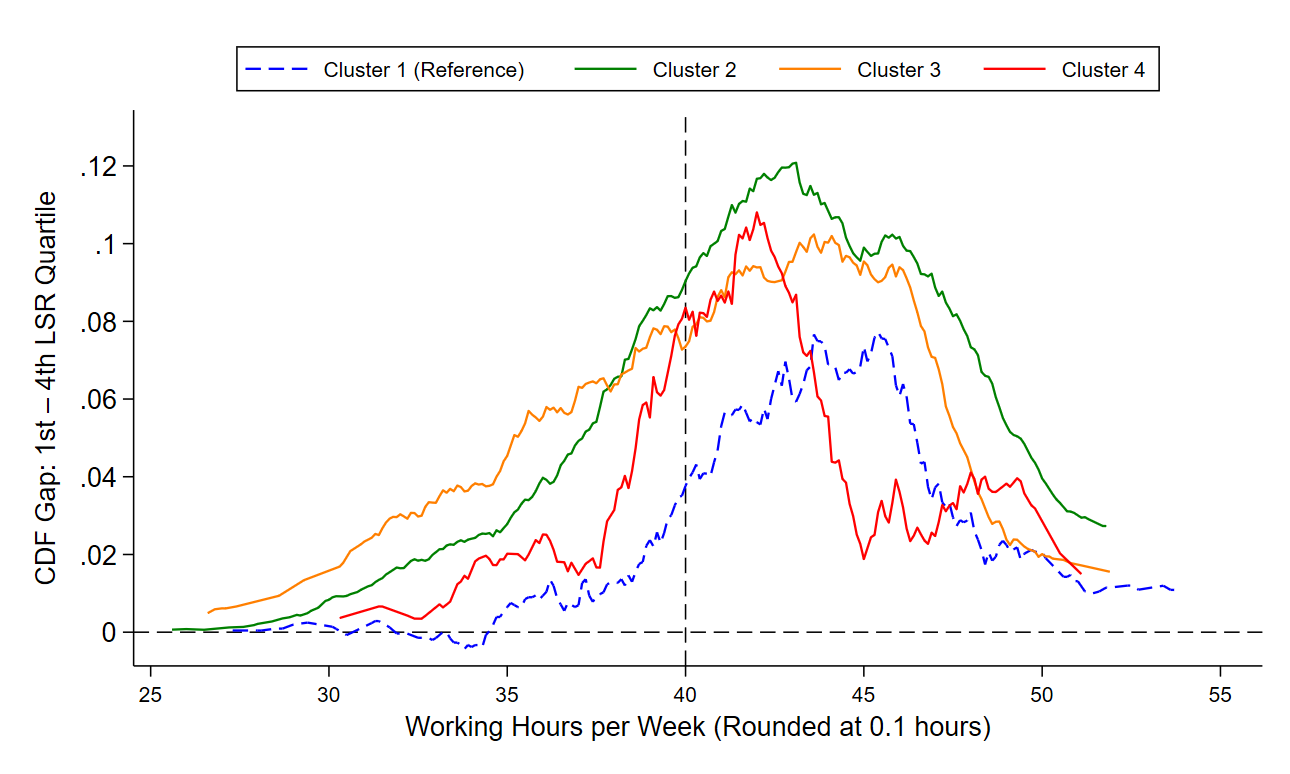
\includegraphics[keepaspectratio]{Share of Compliance.png}}
\caption{Average Causal Effects Based on CDF Gaps in Working Hours (by
Cluster)}
\end{figure}

Figure 8 illustrates the compliance pattern by showing how instrumented
treatment intensity varies across monotonic IV strata by visualizing the
CDF gap in working hours rounded at 0.1 hours on each cluster between
the lowest and highest quartiles. At a glance, the bulk of average
causal responses appears concentrated above 40 hours, the institutional
threshold for full-time work. As proven by the quasi-absence of a
negative CDF gap in each cluster, presenting monotonic effects of IV
satisfy key identifying assumptions of causal inference except minimal
negative values reported between 30 to 35 hours per week in the
reference group (Cluster 1). The ranking of compliance shares aligns
with the results in Table 10: Cluster 2, where the most elastic to
working hours by labor shortage rate variations, has the largest range
in the share of compliance. Despite Cluster 4 reporting a distinctive
peak among the gaps of other clusters, the narrow range of working hours
where the gap is non-negligible may reflect estimated results at the
first stage: The most distinctive between-effects presence with the
weakest within-responsiveness. The weak compliance pattern observed in
Cluster 1 is consistent with the statistically insignificant estimates
in the first-stage regression.

\FloatBarrier
\begin{table}[!h]
\centering\centering
\caption{\label{tab:unnamed-chunk-18}2SPS-IV Estimates of Overtime Effects on Job Satisfaction (Equation 4.7 and 4.8)}
\centering
\resizebox{\ifdim\width>\linewidth\linewidth\else\width\fi}{!}{
\fontsize{11}{13}\selectfont
\begin{threeparttable}
\begin{tabular}[t]{lcc}
\toprule
Variable & (1) & (2)\\
\midrule
Main Explanatory Variable (Fitted) &  & \\
\hline
Overtime Worker X Weekly Working Hours &  & -0.0050***\\
 &  & (0.0014)\\
Weekly Working Hours & -0.2008 & -0.1909\\
 & (0.1470) & (0.1471)\\
\addlinespace
Weekly Working Hours (Squared) & 0.0018 & 0.0018\\
 & (0.0014) & (0.0014)\\
\hline
Control Variable &  & \\
\hline\\
Hourly Wage & 0.0306 & 0.0300\\
 & (0.0206) & (0.0206)\\
\addlinespace
Age & 0.0077 & 0.0067\\
 & (0.0102) & (0.0101)\\
Years of Education & -0.0539 & -0.0512\\
 & (0.0957) & (0.0957)\\
Household Size & -0.0684** & -0.0681**\\
\addlinespace
 & (0.0248) & (0.0248)\\
Marital Status & 0.1476* & 0.1618*\\
 & (0.0715) & (0.0714)\\
Household Income & 0.0000 & 0.0000\\
 & (0.0002) & (0.0002)\\
\addlinespace
Temporary Contract & -0.2308** & -0.2372**\\
 & (0.0758) & (0.0760)\\
Atypical Contract & -0.4407*** & -0.4574***\\
 & (0.1328) & (0.1331)\\
Paid Vacation Provided & 0.3760*** & 0.3782***\\
\addlinespace
 & (0.0663) & (0.0664)\\
Public-Sector Employer & 0.2738** & 0.2745**\\
 & (0.0940) & (0.0940)\\
Years of Tenure & 0.0001 & 0.0006\\
 & (0.0084) & (0.0084)\\
\hline
\addlinespace
Pseudo-Observations & 657681 & 657681\\
Observations & 49643 & 49643\\
Number of Individuals & 9368 & 9368\\
Pseudo R-Squared & 0.6251 & 0.6253\\
Log conditional Likelihood & -103999.49 & -103950.32\\
\bottomrule
\end{tabular}
\begin{tablenotes}
\item[1] All coefficients are expressed in log-odds. Standard errors clustered at the individual level are reported in parentheses.
\item[2] Expanded through BUC-OLOGIT estimation (Baetschmann et al., 2020).
\item[3] Observations with multiple positive outcomes within groups are excluded due to identification constraints.
\item[4] All models control for industry, occupational category, firm region, and firm size.
\item[5] * p<0.05, ** p<0.01,  *** p<0.001
\end{tablenotes}
\end{threeparttable}}
\end{table}

Table 13 reports the IV-2SPS estimation results from Equations 4.7 and
4.8. Compared to previous specifications, the only statistically
significant effect appears in the interaction term between overtime
status and fitted weekly working hours. The interaction term between
overtime status and fitted weekly working hours indicates that, for
overtime workers, each additional hour of work reduces the odds of
reporting higher job satisfaction by approximately 0.5\%, with strong
statistical significance at the 0.1\% level. Since these IV-based
estimates reflect the population odds ratio (POR) among compliers, those
whose working hours are causally affected by industry-level labor
shortages, the results demonstrate how enforced overtime leads to a
deviation from optimal utility levels (Burgess, 2013). The risk of
burnout increases with the accumulation of fatigue, particularly when
workers are unable to shift into occupations offering more adaptable
schedules (Hart, 2004; Rätzel, 2012; Jacobs \& Piyapromdee, 2016;
Pencavel, 2016b; Donsimoni, 2020). Contrary to Rätzel (2012), the
non-pecuniary utility associated with working hours appears less salient
under conditions of labor market constraint, as the concavity of the
utility function is statistically insignificant when working hours are
instrumented by exogenous variation\footnote{Despite its statistical
  insignificance, a convex-like presentation from the second-order
  derivative of the working hour function might create confusion in its
  interpretation. However, the curvature difference made by IV-2SPS
  estimation relies on the local segment relative to its identification
  region. The global shape of the functional structure still aligns with
  the second stage of baseline estimation, suggested by Equations 4.4
  and 4.5.}.

As suggested by several studies on recovery from work-induced fatigue,
paid leave exhibits a strong positive effect as an institutional
guarantee of relaxation, increasing the probability of higher job
satisfaction by approximately 45.64 (column 1) to 45.97 (column 2)
percentage points in odds ratio\footnote{The actual effects of recovery
  from work-driven fatigue are assumed to be gradual. Yet the treatment
  of paid vacation offered by establishments only indicates a
  dichotomous response. It is important to note that such coefficients
  only indicate the average response of the related individuals compared
  to others.}, rounded to three decimal places (Jacobs \& Piyapromdee,
2016; Pencavel, 2016b; Donsimoni, 2020). In contrast, the effect of
hourly wages is no longer statistically significant and reports only a
minimal coefficient compared to the results from the baseline
second-stage estimation. This shift suggests that the previously assumed
selection bias, where workers with stronger financial incentives
voluntarily choose to work overtime, becomes less relevant once working
hours are instrumented by exogenous variation reflecting
constraint-driven labor supply.

Indeed, several studies argue that economic incentives such as overtime
premiums can induce excessive working hours in income-effects-responsive
individuals (Park \& Park, 2019; Lim \& Lee, 2024). However, the related
variables to such determinants become less salient when workforce
shortages are predominant in the relevant labor market. The IV-2SPS
estimation results in Table 13 provide robust evidence for the central
hypothesis of this study: externally imposed excessive working hours
have a direct causal effect on reduced job satisfaction among workers.
From the perspective of statistical inference, the 2SPS-IV framework
appears to effectively correct for potential biases stemming from
endogenous variation in individual working hour determination.

In addition to the interpretations on working hours and compensation,
household characteristics and marital status also show a significant
relationship with job satisfaction (Simpson et al., 2024). Each
additional household member is associated with a decrease in
satisfaction probability by approximately 6.58\%p (column 2) to 6.61\%p
(column 1), while having a spouse, an indicator of marital stability,
increases the odds by 15.90\%p (column 1) to 17.56\%p (column 2). In a
similar vein, variables related to employment contract type or workplace
characteristics also yield significant effects. The presence of
irregular contracts (e.g., temporary or atypical) consistently reduces
satisfaction, while employment in the public sector appears to enhance
it. These findings suggest that not only the quantity of work but also
the structural and institutional context in which individuals work serve
as significant determinants in shaping their perception of job
satisfaction.

Taken together, the IV results plausibly reject the idea that the
disutility from long working hours can be compensated. Instead, they
suggest that enforced overwork under labor market constraints leads to
utility losses at the conduction of a static model, consistent with the
burnout-recovery process. From the perspective of the inverse-U-shaped
association between working hours and individual utility, this study
clarifies that overtime-induced disutility exists when such
participation is affected by a workforce shortage in the corresponding
labor markets (see Rätzel, 2012). This paper does not negate a
foundational assumption that incentives can cause biased working hour
determinations but clarifies that there is a decline in individual
utility due to excessive working hours under instrumented results.

\newpage

\section{DISCUSSION}\label{discussion}

This study empirically identified the causal pathway from labor shortage
to burnout through a two-stage estimation strategy. In the first stage,
labor shortage rates were found to increase overall working hours and
the likelihood of overtime participation, rather than alter the
allocation of hours across workdays. The magnitude of this effect varied
across industrial clusters, which were constructed using hierarchical
clustering based on the time-series profiles of labor shortage. Notably,
the sensitivity of working hours to labor shortage was inversely ordered
to the average shortage level in each cluster, suggesting differences in
institutional or behavioral responses under varying labor market
conditions.

These first-stage estimates served as the basis for instrumenting
predicted working hours in the second-stage IV-2SPS estimation. By
comparing outcomes from observed and instrumented regressors, the study
successfully isolated the causal effect of enforced overwork on job
satisfaction. While the observational models revealed an
inverse-U-shaped relationship between weekly working hours and
satisfaction, the IV-based results painted a different picture: only
overtime workers experienced significant disutility, and the magnitude
of this effect grew with the predicted level of weekly working hours.
This finding indicates that involuntary overwork, driven by structural
labor market constraints, leads to a measurable loss in individual
utility, independent of endogenous factors such as reverse causality
(e.g., presenteeism) or institutional incentives.

The fitted values from the first-stage model reflect structural
constraints rather than endogenous preferences as provided by IV-2SPS
estimation. Only overtime assigned under shortage pressure causes
significant utility loss, in line with the arguments in the Theoretical
Framework. Besides internal optimization, both the theoretical and
empirical frameworks highlight the same mechanism of constrained
optimization under shortage, fatigue outweighs pecuniary benefits or
non-pecuniary resources beyond 40 hours per week, the legal full-time
reference line. These findings imply that burnout arises from exposure
to excessive working hours within a lack of choice and constrained
recovery. Such empirical evidence might be relative to the issues that
matching frictions lead to the over-utilization of constrained workers
under the monopsonistic environment of the labor market.

This paper raises doubt on the belief that only further institutional
reforms, such as stricter hour limits or formal reference shifts (e.g.,
a 4-day workweek as recently discussed), can fundamentally resolve the
over-employment problem in Korea. As presenting empirical estimation
shows, overtime is frequently induced by market constraint, not only by
labor institutions or incentive-driven internal motivation. Except for
several industries in Cluster 1 (i.e., energy supply, financial,
insurance, real estate, and education services), a majority of workers
are significantly affected by labor shortages in their working hour
decisions. Regarding the entire process of estimation, overtime with
workforce deficit is less relevant to the shift of reference indicating
full-time workers or strict enforcement of working hour regulations.
Unless rigid labor market friction is structurally relaxed, it is
difficult to reduce long and unproductive working hours in the long run.
Thus, when considering the root cause of overtime use and its negative
impact, structural compulsion under a constrained labor allocation
system needs to be alleviated.

Moreover, due to the decline in the number of economically active
populations in Korea, labor supply constraints will also be enhanced
(i.e., low birth rates and an aging population). As Jang (2018) argues,
the misallocation of the workforce within market inefficiency might be
aggravated by the projection of diminishing demographic bonuses. As
descriptive statistics of this paper present, the labor market
polarization problem might be partially relevant to the aforementioned
rigid labor market friction. While this study only examines employed
individuals from 2009 to 2023, the observed polarization in labor market
outcomes seemingly suggests that rigid labor market frictions remain a
barrier to efficient allocation. In particular, the limited distribution
of stable wage-and-salary jobs and the slow improvement in working
conditions for the working-age population highlight deeper structural
challenges with their alleviation.

Given the structural constraint posed by persistent labor market
segmentation, this study suggests public support for the improvement of
working conditions in SMEs. According to descriptive statistics across
industries, both higher shortage rates and longer working hours are
mainly recorded in small-sized firms. As OLFSE provides the reasons for
unfilled jobs from the aspect of firms, it is mostly related to the
hiring pressure: lack of job seekers with the required skills,
difficulty in providing working conditions as desired demands from
potential candidates, and the competition among employers in a similar
labor market. Barnow et al.~(2013) suggest allowing entry-level
practitioners to be hired in occupations to gain human capital in
contrast to the tightened labor market circumstance. Subsequently,
enhancing labor productivity can mitigate both workforce deficit and
long working hour problems. M. Kim (2024) also suggests flexible work
arrangement that adapts to upcoming technical progress. Therefore,
promoting flexibility with vocational training might enhance both labor
productivity and improve long-term labor allocation unless an
excessively concentrated working schedule is encouraged without
sufficient recovery.

\newpage

\section{CONCLUSION}\label{conclusion}

This paper clarified the causal effect of overtime work on the gradual
diminution of individual job satisfaction. As job satisfaction indicates
a perception of employed individuals relative to occupational stress, it
aligns with a path of burnout within the investigation of 15 years of
panel data from 2009 to 2023 in Korea. In contrast to the potential
endogenous property, the internal decision to overtime induced by
incentives, stems from the predominant degree of market constraint as an
instrumental variable through Two-staged Predictor Estimation. A 1\%p
increase in labor shortage rates has an impact of increasing 0.1573
working hours on average, based on the results of the cluster-interacted
term, except for less labor-intensive industries (e.g., financial and
insurance services). Through a non-linear estimation, the association
between working hours and individual job satisfaction varies as an
inversed-U-shape, maximized around the full-time reference, but its
causal effects induced by instruments are equal to a 0.5\%p decrease in
odds per hour of work for overtime workers. Thus, overtime work is a
causal determinant of burnout exposure under pressure of workforce
shortage across the labor market.

Based on the probability distribution of observed individual working
hours, empirical investigation for overtime work relies on the right
tail of the entire random variable set. Since the Ordinary Least Square
(OLS) method follows the Central Limit Theorem (CLT) relative to the Law
of Large Numbers (LLN), local identification, focused on overtime
workers serving at the points above the mean value of the entire working
hour distribution, in the first stage estimates had difficulty
overcoming such convergence problems. Hence, this study acknowledges
methodological limitations regarding potentially underpowered estimates:
Right-tail risk of identification between 40 hours per week to the
entire disposable weekly time. Quantile Treatment Effects (QTE) may
provide less restricted results, finding coefficients between predictors
and their responses from specific quantiles as an alternative approach.
However, this study prioritized estimating baseline proportional
responses on the latent utility scale based on comparison at the
overtime threshold. Aforementioned issues will be corrected in further
phase of research.

Despite the difficulties mentioned above, this study contributes to
providing causal evidence that overtime exposure impacts individual
negative outcomes, particularly on their subjective perception.
Methodologically, the present analysis applies odds-based calculation
under the Average Causal Response theorem within a burnout framework, an
approach scarcely explored in existing literature. Compared to the
traditional belief that occupational fatigue is mostly considered
unobserved individual irresponsible characteristics, this paper
ultimately claims that inevitable overtime imposition due to market
constraint might lead to individual burnout. Still, the need for further
research remains: Since burnout symptoms are heavily related to
accumulated occupational fatigue, a further suggestible investigation
incorporates dynamic equations specifying the degree of burnout-related
behaviors and phases of overtime exposures (e.g., Heckman Selection
Model including corner solution). In conclusion, I emphasize the need
for structural adjustments to the rigid labor market of Korea, rather
than relying solely on further institutional enforcement to address long
and inefficient working hour practices.

\newpage

\section*{BIBLIOGRAPHY}\label{bibliography}
\addcontentsline{toc}{section}{BIBLIOGRAPHY}

\let\oldprintbibliography\printbibliography
\renewcommand{\printbibliography}{\oldprintbibliography}

\printbibliography[heading=none]

\newpage

\section*{APPENDIX}\label{appendix}
\addcontentsline{toc}{section}{APPENDIX}

\renewcommand{\printbibliography}{}

\appendix

\renewcommand{\thefigure}{A\arabic{figure}}
\renewcommand{\thetable}{A\arabic{table}}
\setcounter{figure}{0}
\setcounter{table}{0}

\begin{figure}
\centering
\pandocbounded{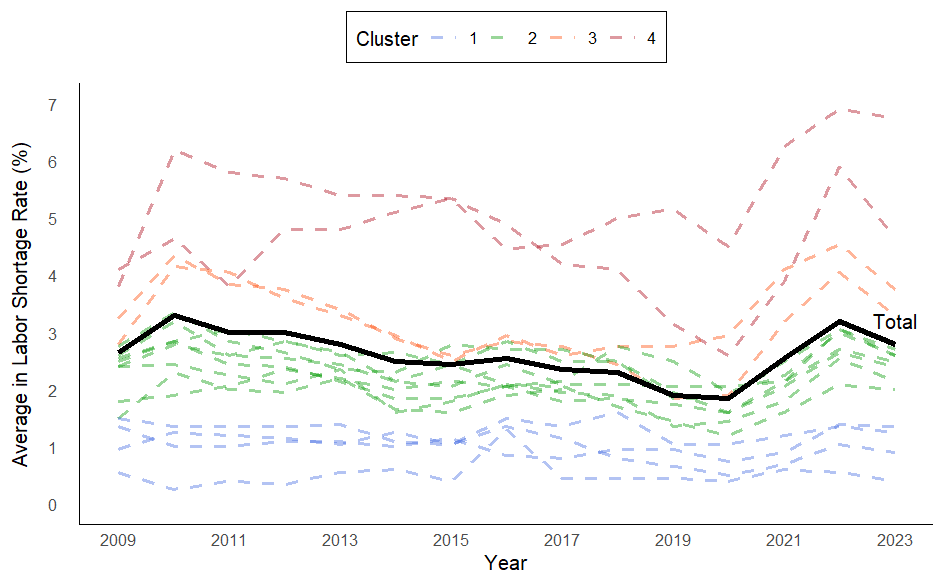
\includegraphics[keepaspectratio]{000010.png}}
\caption{Average Labor Shortage Rate by Industry
(2009\textasciitilde2023)}
\end{figure}

\begin{figure}
\centering
\pandocbounded{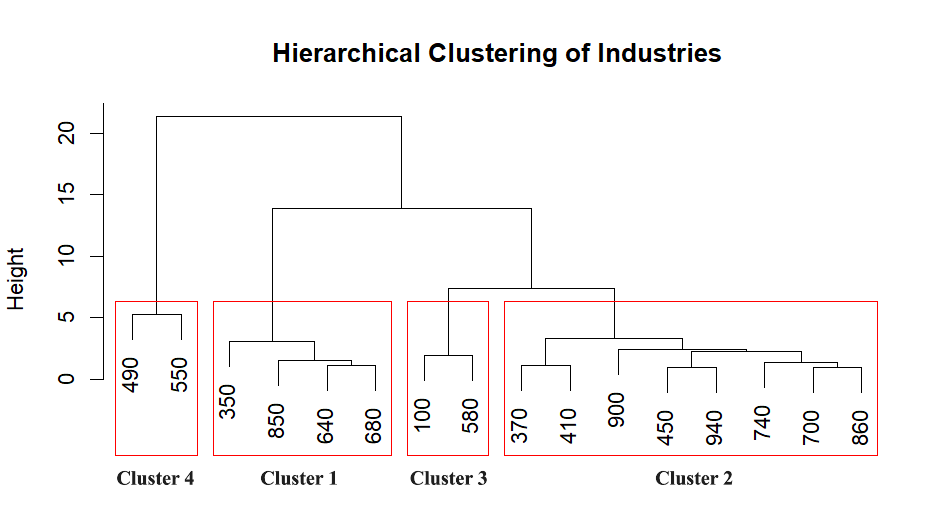
\includegraphics[keepaspectratio]{00001e.PNG}}
\caption{Cluster Dendrogram of Labor Shortage Rates
(2009\textasciitilde2023)}
\end{figure}

\begin{landscape}\begingroup\fontsize{11}{13}\selectfont

\begin{ThreePartTable}
\begin{TableNotes}
\item[1] In the description column, the code of original variables from raw data below each cell is inscribed to specify how variables are defined in this study.
\end{TableNotes}
\begin{longtable}[t]{ll>{\raggedright\arraybackslash}m{12.5cm}}
\caption{\label{tab:unnamed-chunk-21}Definition of Variables (KLIPS)}\\
\toprule
Name of Variable & Type & Description\\
\midrule
\endfirsthead
\caption[]{Definition of Variables (KLIPS) \textit{(continued)}}\\
\toprule
Name of Variable & Type & Description\\
\midrule
\endhead

\endfoot
\bottomrule
\insertTableNotes
\endlastfoot
\cellcolor{gray!10}{Time-Invariant} & \cellcolor{gray!10}{} & \cellcolor{gray!10}{}\\
\hline\noalign{\vskip -0.1ex}
Female & Nominal (Dummy, 0/1) & =1 if individual is female (p\_0101)\\
\hline\noalign{\vskip -0.1ex}
\cellcolor{gray!10}{Time-Variant} & \cellcolor{gray!10}{} & \cellcolor{gray!10}{}\\
\hline\noalign{\vskip -0.1ex}
Job Satisfaction & Ordinal (21 bins) & Averaged scores of five subcomponents in job satisfaction with 5-likert scale (p\_4311, p\_4313, p\_4314, p\_4315, p\_4317)\\
\cellcolor{gray!10}{Weekly Working Hours} & \cellcolor{gray!10}{Continuous} & \cellcolor{gray!10}{Total weekly hours worked, including overtime (p\_1004, p\_1006, p\_1012, p\_1019).}\\
\addlinespace
Weekly Working Days & Discrete (1-7 Days) & Total workdays per week, including overtime days (p\_1005, p\_1007, p\_1013, p\_1019).\\
\cellcolor{gray!10}{Daily Working Hours} & \cellcolor{gray!10}{Continuous} & \cellcolor{gray!10}{Computed as Weekly Working Hours / Working Days per Week (Derived).}\\
Overtime Worker & Nominal (Dummy, 0/1) & =1 if total weekly working hours exceed the legal threshold of 40 hours\\
\cellcolor{gray!10}{Hourly Wage} & \cellcolor{gray!10}{Continuous (1,000 KRW per hour)} & \cellcolor{gray!10}{Computed as: Monthly Wage / (Weekly Working Hours x 4.3)}\\
Monthly Wage & Continuous (10,000 KRW per Month) & Self-reported average values of monthly wage during a year of survey. (p\_1642)\\
\addlinespace
\cellcolor{gray!10}{Age} & \cellcolor{gray!10}{Continuous (Years)} & \cellcolor{gray!10}{Age of respondent (p\_0107)}\\
Years of Education & Continuous (Years) & Total years of schooling completed with respect to graduation status (based on p\_0110, p\_0112)\\
\cellcolor{gray!10}{Household Size} & \cellcolor{gray!10}{Discrete} & \cellcolor{gray!10}{Number of people in the household (h\_0150)}\\
Marital Status & Nominal (Dummy, 0/1) & =1 if individual is currently having a spouse (based on p\_5501)\\
\cellcolor{gray!10}{Household Income} & \cellcolor{gray!10}{Continuous (10,000 KRW per Month)} & \cellcolor{gray!10}{Household income excluding labor income (sum of h\_2204, h\_2206, h\_2208, h\_2210, h\_2212 without missing values)}\\
\addlinespace
Temporary Contract & Nominal (Dummy, 0/1) & =1 if a fixed-term worker (p\_0501=1), meaning the employment contract specifies a set duration\\
\cellcolor{gray!10}{Atypical Contract} & \cellcolor{gray!10}{Nominal (Dummy, 0/1)} & \cellcolor{gray!10}{=1 if employed under non-standard work arrangements, such as dispatch work (p\_0611=2), subcontracting (p\_0611=3), independent contracting (p\_0612=1), remote work (p\_0613=1), or casual (daily) work (p\_0508=1)}\\
Paid Vacation Provided & Nominal (Dummy, 0/1) & =1 if employer offers paid vacation (p\_4105)\\
\cellcolor{gray!10}{Public-Sector Employer} & \cellcolor{gray!10}{Nominal (Dummy, 0/1)} & \cellcolor{gray!10}{=1 if working in a public institution, government agency, or state-owned enterprise (p\_0401=3 or 5).}\\
Years of Tenure & Continuous (Years) & Total years worked in the current job from the year of entrance (p\_0301) until the year of survey\\
\addlinespace
\cellcolor{gray!10}{Level of Job Skill} & \cellcolor{gray!10}{Ordinal (3 bins)} & \cellcolor{gray!10}{Categorized based on occupational classification (p\_0352): 1 = Low-skilled (service, sales, manual work), 2 = Middle-skilled (clerical, technical, machine operation), 3 = High-skilled (managers, professionals).}\\
Industry & Nominal (16 categories) & Industry classification based on KSIC by section (p\_0341)\\
\cellcolor{gray!10}{Size of Firm} & \cellcolor{gray!10}{Ordinal (5 bins)} & \cellcolor{gray!10}{Classifying the size of firm as a number of employed individuals except government organizations: 5\textasciitilde{}9, 10\textasciitilde{}29, 30\textasciitilde{}99, 100\textasciitilde{}299, and More or equal to 300 (p\_0402, p\_0403)}\\
Region of Firm Location & Nominal (17 regions) & Workplace location by administrative region (p\_0311)\\*
\end{longtable}
\end{ThreePartTable}
\endgroup{}
\end{landscape}

\begin{landscape}\begin{table}[!h]
\centering\centering
\caption{\label{tab:unnamed-chunk-22}Descriptive Statistics of Labor Shortage Rate}
\centering
\resizebox{\ifdim\width>\linewidth\linewidth\else\width\fi}{!}{
\fontsize{11}{13}\selectfont
\begin{threeparttable}
\begin{tabular}[t]{lcccccccccccccccc}
\toprule
Code of Industrial Categories & 100 & 350 & 370 & 410 & 450 & 490 & 550 & 580 & 640 & 680 & 700 & 740 & 850 & 860 & 900 & 940\\
\midrule
Average Labor Shortage Rate & 3.087 & 0.513 & 1.9 & 1.944 & 2.573 & 5.039 & 4.735 & 3.297 & 1.039 & 1.003 & 2.145 & 2.252 & 1.297 & 2.337 & 2.238 & 2.558\\
 & {}[0.711] & {}[0.233] & {}[0.255] & {}[0.361] & {}[0.346] & {}[0.851] & {}[1.044] & {}[0.632] & {}[0.190] & {}[0.240] & {}[0.365] & {}[0.501] & {}[0.172] & {}[0.251] & {}[0.321] & {}[0.424]\\
\hline\noalign{\vskip -0.1ex}
Size of Firm &  &  &  &  &  &  &  &  &  &  &  &  &  &  &  & \\
\hline\noalign{\vskip -0.1ex}\\
- 5 \textasciitilde{} 9 employees & 5.688 & 0.819 & 3.089 & 2.512 & 3.297 & 1.919 & 5.074 & 5.82 & 0.937 & 1.173 & 3.124 & 3.184 & 2.996 & 2.824 & 3.143 & 3.423\\
 & {}[2.377] & {}[2.241] & {}[2.293] & {}[1.639] & {}[1.633] & {}[1.809] & {}[2.448] & {}[3.333] & {}[1.116] & {}[1.438] & {}[1.665] & {}[2.508] & {}[1.706] & {}[1.348] & {}[2.752] & {}[1.909]\\
\addlinespace
- 10 \textasciitilde{} 29 employees & 4.21 & 0.894 & 1.967 & 1.778 & 2.265 & 4.021 & 4.47 & 3.338 & 0.65 & 0.809 & 2.194 & 2.658 & 1.539 & 2.224 & 2.252 & 2.449\\
 & {}[1.619] & {}[1.474] & {}[1.429] & {}[1.014] & {}[1.018] & {}[4.269] & {}[2.194] & {}[1.792] & {}[0.670] & {}[1.251] & {}[1.097] & {}[1.926] & {}[1.190] & {}[1.034] & {}[1.849] & {}[1.401]\\
- 30 \textasciitilde{} 99 employees & 2.978 & 0.591 & 1.118 & 1.456 & 1.676 & 7.075 & 3.985 & 1.666 & 0.82 & 1.235 & 1.763 & 1.92 & 0.548 & 2.39 & 1.697 & 1.57\\
 & {}[1.326] & {}[0.930] & {}[1.076] & {}[1.264] & {}[1.122] & {}[4.393] & {}[2.597] & {}[1.769] & {}[0.917] & {}[2.170] & {}[1.117] & {}[1.332] & {}[0.775] & {}[1.002] & {}[1.187] & {}[1.276]\\
- 100 \textasciitilde{} 299 employees & 1.795 & 0.415 & 0.271 & 1.139 & 1.129 & 3.579 & 2.454 & 1.084 & 0.849 & 0.639 & 1.722 & 1.75 & 0.884 & 2.382 & 1.137 & 0.79\\
\addlinespace
 & {}[1.137] & {}[0.949] & {}[1.058] & {}[1.745] & {}[0.989] & {}[2.925] & {}[2.410] & {}[1.464] & {}[2.165] & {}[1.530] & {}[1.750] & {}[1.396] & {}[2.148] & {}[1.244] & {}[1.602] & {}[1.586]\\
- 300 or more employees & 0.71 & 0.268 & 0.0278 & 0.464 & 0.452 & 1.34 & 1.024 & 0.954 & 0.486 & 0.536 & 0.985 & 1.547 & 0.863 & 1.814 & 0.701 & 0.48\\
 & {}[0.726] & {}[0.918] & {}[0.243] & {}[1.233] & {}[0.935] & {}[1.869] & {}[2.856] & {}[1.821] & {}[1.440] & {}[1.288] & {}[1.214] & {}[1.749] & {}[1.715] & {}[1.411] & {}[2.059] & {}[1.662]\\
\hline\noalign{\vskip -0.1ex}
Region of Firm Location &  &  &  &  &  &  &  &  &  &  &  &  &  &  &  & \\
\hline\noalign{\vskip -0.1ex}\\
- capital area & 3.144 & 0.707 & 1.313 & 1.651 & 2.441 & 4.934 & 3.752 & 3.882 & 1.19 & 0.995 & 2.553 & 2.828 & 1.325 & 2.429 & 2.23 & 2.253\\
\addlinespace
 & {}[1.981] & {}[0.888] & {}[1.675] & {}[1.178] & {}[1.153] & {}[4.241] & {}[2.295] & {}[2.300] & {}[1.199] & {}[0.751] & {}[1.344] & {}[1.883] & {}[1.091] & {}[1.042] & {}[1.975] & {}[1.528]\\
- metropolitan cities & 2.69 & 0.544 & 1.15 & 1.453 & 1.466 & 3.58 & 2.92 & 2.356 & 0.735 & 0.681 & 1.764 & 1.869 & 1.198 & 1.853 & 1.43 & 1.573\\
 & {}[2.211] & {}[1.632] & {}[1.756] & {}[1.609] & {}[1.345] & {}[4.420] & {}[2.754] & {}[2.748] & {}[1.163] & {}[1.243] & {}[1.521] & {}[1.703] & {}[1.527] & {}[1.151] & {}[1.786] & {}[1.954]\\
- other provinces & 3.414 & 0.617 & 1.417 & 1.438 & 1.859 & 3.239 & 3.753 & 2.426 & 0.645 & 1.03 & 1.979 & 2.365 & 1.531 & 2.737 & 1.998 & 1.764\\
 & {}[2.470] & {}[1.315] & {}[1.834] & {}[1.598] & {}[1.678] & {}[2.927] & {}[3.121] & {}[2.911] & {}[1.557] & {}[1.980] & {}[1.611] & {}[2.075] & {}[2.147] & {}[1.259] & {}[2.409] & {}[1.948]\\
\bottomrule
\end{tabular}
\begin{tablenotes}
\item[1] Standard deviation is in brackets.
\item[2] Average value in labor shortage rate is calculated as national level by industries from 2009 to 2023.
\item[3] Descriptive results is from the information seprately calculated by industries, province level and size of firm.
\end{tablenotes}
\end{threeparttable}}
\end{table}
\end{landscape}

\begin{table}[!h]
\centering\centering
\caption{\label{tab:unnamed-chunk-23}Summary Statistics on Each Domain of Job Satisfaction}
\centering
\resizebox{\ifdim\width>\linewidth\linewidth\else\width\fi}{!}{
\fontsize{11}{13}\selectfont
\begin{threeparttable}
\begin{tabular}[t]{lccc}
\toprule
Domain of Job Satisfaction & Non-Overtime Worker & Overtime Worker & Total\\
\midrule
Composited Level & 3.432 & 3.230 & 3.367\\
(Average) & {}[0.488] & {}[0.511] & {}[0.504]\\
\hline\noalign{\vskip -0.1ex}
Wage & 3.115 & 2.959 & 3.065\\
 & {}[0.679] & {}[0.700] & {}[0.690]\\
Value of Work & 3.539 & 3.397 & 3.493\\
\addlinespace
 & {}[0.612] & {}[0.633] & {}[0.622]\\
Working Environment & 3.475 & 3.261 & 3.406\\
 & {}[0.625] & {}[0.657] & {}[0.643]\\
Working hours & 3.569 & 3.175 & 3.442\\
 & {}[0.599] & {}[0.739] & {}[0.673]\\
\addlinespace
Quality of Communication & 3.462 & 3.356 & 3.428\\
 & {}[0.593] & {}[0.604] & {}[0.598]\\
\hline\noalign{\vskip -0.1ex}
Observations & 35,507 & 16,911 & 52418\\
\bottomrule
\end{tabular}
\begin{tablenotes}
\item[1] Standard deviations in brakets.
\end{tablenotes}
\end{threeparttable}}
\end{table}

\begin{table}[!h]
\centering\centering
\caption{\label{tab:unnamed-chunk-24}Decomposition of Working Hours into Daily Hours and Workdays (Equation 4.4a)}
\centering
\resizebox{\ifdim\width>\linewidth\linewidth\else\width\fi}{!}{
\fontsize{10.5}{12.5}\selectfont
\begin{threeparttable}
\begin{tabular}[t]{lcccc}
\toprule
Variable & (1) & (2) & (3) & (4)\\
\midrule
Main Explatory Variable &  &  &  & \\
\hline\noalign{\vskip -0.1ex}\\
Daily Working Hours & -0.0440*** & 0.1080** & -0.0489*** & 0.0642\\
 & (0.0104) & (0.0346) & (0.0104) & (0.0354)\\
Daily Working Hours (Squared) &  & -0.0077*** &  & -0.0057***\\
 &  & (0.0017) &  & (0.0017)\\
\addlinespace
Weekly Working Days & 0.0028 & 0.0051 & 0.7964*** & 0.7171***\\
 & (0.0218) & (0.0217) & (0.1166) & (0.1192)\\
Weekly Working Days (Squared) &  &  & -0.0766*** & -0.0688***\\
 &  &  & (0.0110) & (0.0112)\\
\hline\noalign{\vskip -0.1ex}
Control Variable &  &  &  & \\
\hline\noalign{\vskip -0.1ex}\\
\addlinespace
Hourly Wage & 0.0493*** & 0.0507*** & 0.0492*** & 0.0502***\\
 & (0.0046) & (0.0045) & (0.0046) & (0.0045)\\
Age & 0.0075 & 0.0068 & 0.0056 & 0.0053\\
 & (0.0055) & (0.0054) & (0.0055) & (0.0054)\\
Years of Education & -0.1022 & -0.1073 & -0.1060 & -0.1094\\
\addlinespace
 & (0.0579) & (0.0579) & (0.0584) & (0.0583)\\
Household Size & -0.0683** & -0.0685** & -0.0692** & -0.0692**\\
 & (0.0243) & (0.0243) & (0.0243) & (0.0243)\\
Marital Status & 0.1355 & 0.1406* & 0.1351 & 0.1391*\\
 & (0.0702) & (0.0701) & (0.0701) & (0.0701)\\
\addlinespace
Household Income & 0.0002 & 0.0002 & 0.0002 & 0.0002\\
 & (0.0002) & (0.0002) & (0.0002) & (0.0002)\\
Temporary Contract & -0.1427*** & -0.1356*** & -0.1404*** & -0.1356***\\
 & (0.0388) & (0.0389) & (0.0389) & (0.0389)\\
Atypical Contract & -0.2968*** & -0.2889*** & -0.2707*** & -0.2676***\\
\addlinespace
 & (0.0547) & (0.0546) & (0.0548) & (0.0547)\\
Paid Vacation Provided & 0.2989*** & 0.2918*** & 0.2897*** & 0.2853***\\
 & (0.0334) & (0.0334) & (0.0334) & (0.0334)\\
Public-Sector Employer & 0.3104*** & 0.3107*** & 0.3062*** & 0.3068***\\
 & (0.0788) & (0.0785) & (0.0792) & (0.0790)\\
\addlinespace
Years of Tenure & -0.0078 & -0.0089 & -0.0081 & -0.0088\\
 & (0.0047) & (0.0047) & (0.0047) & (0.0047)\\
\hline\noalign{\vskip -0.1ex}
Pseudo-Observations & 658624 & 658624 & 658624 & 658624\\
Observations & 49643 & 49643 & 49643 & 49643\\
Number of Individuals & 9368 & 9368 & 9368 & 9368\\
\addlinespace
Pseudo R-Squared & 0.6250 & 0.6253 & 0.6256 & 0.6257\\
Log conditional Likelihood & -104177.4 & -104104.2 & -104022.8 & -103984.3\\
\bottomrule
\end{tabular}
\begin{tablenotes}
\item[1] All coefficients are expressed in log-odds. Standard errors clustered at the individual level are reported in parentheses.
\item[2] Expanded through BUC-OLOGIT estimation (Baetschmann et al., 2020).
\item[3] Observations with multiple positive outcomes within groups are excluded due to identification constraints.
\item[4] All models control for industry, occupational category, firm region, and firm size.
\item[5] * p<0.05, ** p<0.01,  *** p<0.001
\end{tablenotes}
\end{threeparttable}}
\end{table}

\begin{table}[!h]
\centering\centering
\caption{\label{tab:unnamed-chunk-25}Decomposition of Working Hours into Daily Hours and Workdays (Equation 4.5a)}
\centering
\resizebox{\ifdim\width>\linewidth\linewidth\else\width\fi}{!}{
\fontsize{10}{12}\selectfont
\begin{threeparttable}
\begin{tabular}[t]{lcccc}
\toprule
Variable & (1) & (2) & (3) & (4)\\
\midrule
Main Explatory Variable &  &  &  & \\
\hline\noalign{\vskip -0.1ex}\\
Overtime Worker X Daily Working Hours & -0.0324* & 0.0053 & -0.0795*** & -0.0700***\\
 & (0.0153) & (0.0166) & (0.0169) & (0.0207)\\
Overtime Worker X Weekly Working Days & 0.0171 & -0.0363 & 0.1150*** & 0.0999**\\
 & (0.0230) & (0.0248) & (0.0269) & (0.0334)\\
\addlinespace
Daily Working Hours & 0.0004 & 0.1241*** & 0.0154 & 0.0374\\
 & (0.0174) & (0.0346) & (0.0175) & (0.0369)\\
Daily Working Hours (Squared) &  & -0.0078*** &  & -0.0014\\
 &  & (0.0018) &  & (0.0020)\\
Weekly Working Days & 0.0639 & 0.0894** & 0.9513*** & 0.9072***\\
\addlinespace
 & (0.0329) & (0.0332) & (0.1269) & (0.1446)\\
Weekly Working Days (Squared) &  &  & -0.0970*** & -0.0916***\\
 &  &  & (0.0133) & (0.0156)\\
\hline\noalign{\vskip -0.1ex}
Control Variable &  &  &  & \\
\hline\noalign{\vskip -0.1ex}\\
Hourly Wage & 0.0490*** & 0.0502*** & 0.0498*** & 0.0500***\\
\addlinespace
 & (0.0045) & (0.0045) & (0.0045) & (0.0045)\\
Age & 0.0063 & 0.0056 & 0.0051 & 0.0050\\
 & (0.0054) & (0.0054) & (0.0054) & (0.0054)\\
Years of Education & -0.1060 & -0.1083 & -0.1130 & -0.1130\\
 & (0.0581) & (0.0580) & (0.0585) & (0.0585)\\
\addlinespace
Household Size & -0.0689** & -0.0691** & -0.0694** & -0.0694**\\
 & (0.0243) & (0.0243) & (0.0243) & (0.0243)\\
Marital Status & 0.1377* & 0.1409* & 0.1397* & 0.1402*\\
 & (0.0701) & (0.0701) & (0.0701) & (0.0701)\\
Household Income & 0.0002 & 0.0002 & 0.0002 & 0.0002\\
\addlinespace
 & (0.0002) & (0.0002) & (0.0002) & (0.0002)\\
Temporary Contract & -0.1378*** & -0.1346*** & -0.1317*** & -0.1315***\\
 & (0.0389) & (0.0389) & (0.0390) & (0.0390)\\
Atypical Contract & -0.2889*** & -0.2795*** & -0.2672*** & -0.2667***\\
 & (0.0546) & (0.0546) & (0.0548) & (0.0547)\\
\addlinespace
Paid Vacation Provided & 0.2885*** & 0.2858*** & 0.2781*** & 0.2782***\\
 & (0.0335) & (0.0335) & (0.0334) & (0.0334)\\
Public-Sector Employer & 0.3055*** & 0.3060*** & 0.3048*** & 0.3049***\\
 & (0.0786) & (0.0787) & (0.0790) & (0.0789)\\
Years of Tenure & -0.0082 & -0.0088 & -0.0090 & -0.0091\\
\addlinespace
 & (0.0047) & (0.0047) & (0.0047) & (0.0047)\\
\hline\noalign{\vskip -0.1ex}
Pseudo-Observations & 658624 & 658624 & 658624 & 658624\\
Observations & 49643 & 49643 & 49643 & 49643\\
Number of Individuals & 9368 & 9368 & 9368 & 9368\\
Pseudo R-Squared & 0.625 & 0.625 & 0.626 & 0.626\\
\addlinespace
Log conditional Likelihood & -104118.1 & -104060.1 & -103949.8 & -103948.3\\
\bottomrule
\end{tabular}
\begin{tablenotes}
\item[1] All coefficients are expressed in log-odds. Standard errors clustered at the individual level are reported in parentheses.
\item[2] Expanded through BUC-OLOGIT estimation (Baetschmann et al., 2020).
\item[3] Observations with multiple positive outcomes within groups are excluded due to identification constraints.
\item[4] All models control for industry, occupational category, firm region, and firm size.
\item[5] * p<0.05, ** p<0.01,  *** p<0.001
\end{tablenotes}
\end{threeparttable}}
\end{table}

\printbibliography

\end{document}
